\documentclass[reqno]{article}
\usepackage[margin=.8in]{geometry}
\usepackage{mathtools,amsthm,amssymb}
\usepackage{graphicx,xcolor}
\usepackage[colorlinks, linkcolor=blue!50!black, citecolor=green!40!black, urlcolor=blue!50!black, pagebackref]{hyperref}
\hypersetup{pdftitle={Hilbert functions of filtered graphical zonotopal algebras},pdfauthor={Boris Shapiro; Ilya Smirnov; Arkady Vaintrob}}
\usepackage{rotating}
\usepackage{booktabs,array}
\usepackage{tikz-cd}
\usepackage{tikz}
\usetikzlibrary{positioning}
  \tikzset{vertex/.style={circle,fill,inner sep=1.pt}}

 \usepackage[mathscr]{eucal}  % math script font
\usepackage{enumerate}
\usepackage{needspace}
\usepackage{caption}

%% THEOREMS etc
\theoremstyle{plain} % labeling of theorems etc relative to sections
\newtheorem{theorem}{Theorem}[section]
\newtheorem{proposition}[theorem]{Proposition}
\newtheorem{lemma}[theorem]{Lemma}
\newtheorem{corollary}[theorem]{Corollary}
\newtheorem{conjecture}[theorem]{Conjecture}
\newtheorem{claim}[theorem]{Claim}
\newtheorem{mainthm}{Theorem}
\renewcommand{\themainthm}{\Alph{mainthm}}

\theoremstyle{definition}
\newtheorem{definition}[theorem]{Definition}

\theoremstyle{remark}
\newtheorem{remark}[theorem]{\sc Remark}
\newtheorem{problem}[theorem]{Problem}
\newtheorem{example}[theorem]{\sc Example}

% Math Operators
\renewcommand{\Im}{\mathop\mathrm{Im}\nolimits}
 \DeclareMathOperator{\Spec}{Spec}
 \DeclareMathOperator{\rank}{rk}
 \DeclareMathOperator{\gr}{gr}
 \DeclareMathOperator{\Span}{Span}
 \DeclareMathOperator{\Hom}{Hom}

%% SHORTCUTS
 \newcommand{\mf}{\mathfrak}
 \renewcommand{\sl}{\mathfrak{sl}_2}

\newcommand{\N}{\mathbb{N}}
\newcommand{\R}{\mathbb{R}}
\newcommand{\Z}{{\mathbb{Z}}}
\newcommand{\C}{\mathbb{C}}
\newcommand{\K} {\mathbf{k}}
\renewcommand{\P} {\mathbf{P}}

\newcommand {\CC}{\mathscr{C}}
\newcommand{\cA}{{\mathscr{A}}}
\newcommand{\cB}{\mathscr{B}}
\newcommand{\cF}{\mathscr{F}}
\newcommand{\cK} {\mathscr{K}}
\newcommand{\cG} {\mathscr{G}r}

\newcommand{\al}{\alpha}
\newcommand{\be}{\beta}
\newcommand{\de}{\delta}
\newcommand{\eps}{\epsilon}
\newcommand{\ga}{\gamma}
\newcommand{\Ga}{\Gamma}
\newcommand{\la}{\lambda}
\newcommand{\ze}{\zeta}
\newcommand{\Ups}{\Upsilon}
\newcommand{\La} {\Lambda}
\newcommand{\Si}{\Sigma}
\newcommand{\si}{\sigma}
\newcommand{\ve}{\varepsilon }

\newcommand{\hs}{\mathscr{H}}
\newcommand{\hsb}{\overline{\hs}}
\newcommand{\ds}{\displaystyle}

\numberwithin{equation}{section}

\title{\bf Hilbert functions of filtered graphical zonotopal algebras}

 \author{Boris Shapiro%
 \thanks{Department of Mathematics, Stockholm University, SE-106 91 Stockholm,  Sweden and Department of MCS, Guangdong Technion Israel Institute of Technology,  241 Daxue Road, Jinping District, 515063, Shantou, Guangdong province, China,\
 \texttt{\href{mailto:shapiro@math.su.se}{shapiro@math.su.se}}}
\and
 Ilya Smirnov%
 \thanks{BCAM -- Basque Center for Applied Mathematics, Mazarredo 14, 48009 Bilbao, Spain \quad and \quad IKERBASQUE, Basque Foundation for Science, Plaza Euskadi 5, 48009 Bilbao, Spain,
 \texttt{\href{mailto:ismirnov@bcamath.org}{ismirnov@bcamath.org}}}
\and
 Arkady Vaintrob%
\thanks{Department of Mathematics, University of Oregon, Eugene, OR 97403, USA,
  \texttt{\href{mailto:vaintrob@uoregon.edu}{vaintrob@uoregon.edu}}}}

\date{}

\begin{document}

\maketitle

\begin{abstract}
The external zonotopal algebra of a graph is generated by nilpotent
vertex elements $X_v$ and determines the graphical matroid after deleting
loops. Replacing these generators by $f(X_v)$, for a power series $f(u)$, and filtering by word
length gives a family of filtered algebras. We extend filtered graph
reconstruction from simple graphs to loopless multigraphs without
isolated vertices when the linear and quadratic coefficients of $f$ are
nonzero. Nevertheless, even the family of Hilbert functions indexed by
all polynomials does not determine the graph: two nonisomorphic
ten-vertex trees have the same Hilbert function for every $f$, answering
a question of Nenashev and the first author. For forests and series
whose first nonconstant term has degree $k\ge2$, we give a monomial
presentation indexed by partial score vectors whose entries are divisible
by $k$.

For normalized nondegenerate functions, a boundary-state calculus gives
a common finite parameter partition for all trees of a fixed maximum
degree. In maximum degrees three and four, exact symbolic calculations
identify these partitions by the vanishing of specified coefficients of $f^{-1}$. For functions
with nonzero quadratic coefficient, the same calculus gives explicit
recurrences for attached or connecting paths. Symmetry reductions,
including commuting actions of $\mathfrak{sl}_2$ and the symmetric group
on the leaves of a star, determine the generic Hilbert series of stars
and two-vertex multigraphs and also apply to parallel edges and leaves in larger graphs.
For cycles, we determine the highest-degree term and the first three
nonconstant coefficients in the stable range. A weighted independent-set
formula describes the trace sequence in the remaining conjecture.
\end{abstract}

\tableofcontents

\medskip

\noindent\textbf{2020 Mathematics Subject Classification.}
13A70, 05C25, 05E40, 13A30, 13D40.

\noindent\textbf{Keywords.} Zonotopal algebras, filtered algebras,
Hilbert functions, graph reconstruction, boundary states, Hilbert
stratification.

\section{Introduction}
\label{sec:introduction}

How much information about a graph can be recovered from an algebra
associated with it, and how much remains after the algebra is replaced
by its Hilbert function? The external zonotopal algebra $\CC_G$ gives a
particularly concrete setting for these questions. Its isomorphism type
is equivalent to the graphical matroid of $G$, after deleting loops
\cite{Wa1,N1,Ne}. Thus it recovers which sets of edges are forests, but
not how all the edges meet at vertices. In particular, all trees with
the same number of edges have isomorphic external zonotopal algebras.

Keeping the algebra and changing its filtration can recover the missing
information. Nenashev and the first author \cite{NSh} replaced the nilpotent vertex
generators $X_v$ by $\exp(X_v)$ and filtered by the number of factors in
products of these generators. The resulting filtered algebra determines
a loopless multigraph without isolated vertices
\cite[Theorem~5]{NSh}. For any fixed series with nonzero linear and
quadratic coefficients, they proved the same statement for simple
graphs without isolated vertices \cite[Theorem~6]{NSh}.
Our Theorem~\ref{th:Isom-f} extends this to loopless multigraphs without
isolated vertices. In all these cases the underlying algebra remains
$\CC_G$. Thus the additional information is in the filtration.

These results describe two extremes: the graded algebra retains only
the graphical matroid, whereas an appropriate filtered algebra retains
the whole graph. Direct comparison of filtered algebras, however,
requires both multiplication and filtration data in a space whose
dimension is the number of spanning forests---already $2^N$ for a tree
with $N$ edges. We therefore study the more accessible Hilbert functions
of these filtrations. They require ranks of spaces of products, rather
than the construction or exclusion of algebra isomorphisms. Our main
questions are which graphs they distinguish, how they depend on $f$,
and how they can be computed under graph attachment.

\subsection{Definitions and notation for the results}

Throughout, $\K$ is a field of characteristic zero. Graphs are finite
undirected multigraphs. Loops are allowed, but are excluded from the
degree count and do not affect $\CC_G^f$; they still index variables of
the ambient edge algebra $\Phi_G$. Write $\Delta(G)$
for the maximum non-loop vertex degree. A leaf is a vertex of non-loop degree one; its incident non-loop edge
is a leaf edge. We call vertices of non-loop degrees two and three
bivalent and trivalent, respectively. A tree is connected, and a
forest need not be. In the enumeration statements, a unicyclic graph is
connected and has exactly one cycle. A subcubic graph has maximum degree
at most three.

Choose an orientation of the non-loop edges and put
\[
 \Phi_G=\K[\varphi_e:e\in E(G)]/(\varphi_e^2),\qquad
 X_v=\sum_{e\text{ leaving }v}\varphi_e-
     \sum_{e\text{ entering }v}\varphi_e,\qquad
 \CC_G=\K[X_v:v\in V(G)]\subseteq\Phi_G.
\]
Changing the orientation changes signs of edge variables and gives an
isomorphic algebra. The standard grading assigns degree one to every
$\varphi_e$. The dimension of $\CC_G$ counts spanning forests, and its
graded Hilbert series is a specialization of the Tutte polynomial
\cite{PSS,PS,Wa1}.

For any polynomial or formal power series $f$, put $Y_v=f(X_v)$ and
let $\CC_G^f$ be the subalgebra generated by $1$ and the $Y_v$, with
filtration
\[
 \CC_G^{f,d}=\Span\{Y_{v_1}\cdots Y_{v_j}:0\le j\le d\},\qquad
 \CC_G^{f,-1}=0.
\]
The empty product is $1$. Its \emph{Hilbert function} is the sequence
$h_d(G,f)=\dim(\CC_G^{f,d}/\CC_G^{f,d-1})$, and its \emph{Hilbert
series} is the polynomial
\[
 \hs_G^f(t)=\sum_{d\ge0}h_d(G,f)t^d.
\]
Thus $\dim\CC_G^{f,d}=\sum_{j=0}^d h_j(G,f)$. We use $[t^d]H$ for
the coefficient of $t^d$ in a series $H$, and $\operatorname{lt}_tH$
for its highest-degree term.

Adding a constant to $f$, or multiplying it by a nonzero scalar, does
not change this filtration. A series is \emph{nondegenerate} if
$f'(0)\ne0$; in that case we normalize
\[
 f(u)=u+\alpha u^2+\beta u^3+\gamma u^4+\delta u^5+\cdots,
\]
and $\CC_G^f=\CC_G$ as unfiltered algebras. We write $g=f^{-1}$ for
its compositional inverse. A nonconstant \emph{degenerate} series, after
subtracting its constant term, has the form $cu^k+\cdots$, where
$c\ne0$ and $k\ge2$; its \emph{order} is $k$. If $G$ has a non-loop edge, such a series
generates a proper subalgebra of $\CC_G$. Constant functions give the algebra $\K$.

Since $X_v^{\deg v+1}=0$, only coefficients through degree $\Delta(G)$
matter. For nondegenerate functions we therefore use the parameter space
\[
 \cA_D=\{u+a_2u^2+\cdots+a_Du^D\}\simeq\mathbb A_\K^{D-1},
 \qquad D\ge\max(1,\Delta(G)).
\]
For a fixed graph the Hilbert series is constant on a nonempty Zariski
open subset of this space. This is the \emph{generic Hilbert series};
its cumulative dimensions, not necessarily its individual coefficients,
are maximal \cite[Proposition~3]{NSh}. A \emph{Hilbert stratum} consists
of the parameters giving a specified series. We call a nondegenerate
parameter \emph{Hilbert-exceptional for $G$} if its series is not the
generic one. This terminology makes no assertion about singularities
of the stratum. Here a stratification means a finite partition into
locally closed subsets; no smoothness or frontier condition is imposed
on its parts.

We write $C_n$ for the simple cycle on $n\ge3$ vertices, $S_n$ for the
star $K_{1,n-1}$, and $E_m$ for two vertices joined by $m$ parallel edges.
The tree $T(a,b,c)$ has three paths of edge lengths $a,b,c$ attached at
one common endpoint; in particular $\mathrm D_6=T(1,1,3)$ and $\mathrm E_6=T(1,2,2)$.
A \emph{partial orientation} orients a subset of the edges. Its
\emph{score vector} $a=(a_v)$ counts the selected edges directed away
from each vertex. Let
\[
 s_k(G;t)=\sum_{\substack{a\text{ a partial score vector}\\                         k\mid a_v\ \text{for all }v}}t^{|a|/k},
 \qquad |a|=\sum_v a_v,
\]
where each distinct score vector is counted once, irrespective of the
number of partial orientations producing it. Finally, $h_m^f(t)$
denotes the Hilbert series of $\K[x]/(x^{m+1})$ filtered by products of
$x$ and $f(x)$. These one-variable filtrations enter the star formula below.

For a graph $G$ with marked vertex $v$, let $G_n$ be obtained by attaching
a path with $n$ edges at $v$. For disjoint marked graphs $(G',v')$ and
$(G'',v'')$, let $G'\ast_nG''$ join their marked vertices by such a path.
For a sequence of polynomials put
\[
 L(a_n)=a_n-a_{n-1}-3t\,a_{n-2}+2t\,a_{n-3}.
\]

For a fixed graph, call the map $f\mapsto\hs_G^f$ its
\emph{all-polynomial Hilbert profile} when $f$ ranges over $\K[u]$,
and its \emph{nondegenerate Hilbert profile} when $f'(0)\ne0$.
Equality of profiles always means pointwise equality at the same $f$,
not merely equality of the sets of possible series. Two graphs
are \emph{universally Hilbert equivalent} when their nondegenerate
profiles agree (see Section~\ref{sec:universal-collisions}).

\begin{example}[The path with two edges]\label{ex:two-edge-path}
For the path $1-2-3$, write $a=\varphi_{12}$ and $b=\varphi_{23}$,
with both edges oriented in increasing vertex order. Then
\[
 X_1=a,\quad X_2=b-a,\quad X_3=-b,\qquad
 Y_1=a,\quad Y_2=b-a-2\alpha ab,\quad Y_3=-b.
\]
If $\alpha\ne0$, the ordinary degree-two element $ab$ already belongs
to $\CC_G^{f,1}$. Hence $\hs_G^f=1+3t$, whereas
$\hs_G^u=1+2t+t^2$. This change records when an element can be expressed
in the new generators, not a change in the underlying algebra.
\end{example}

\subsection{Main results}

\paragraph{The limits of Hilbert functions.}
\begin{mainthm}[Failure of all-polynomial reconstruction]\label{thmA}
\leavevmode
\begin{enumerate}[(i)]
\item The two nonisomorphic ten-vertex trees denoted $T3_1,T3_2$ in
Figure~\ref{fig:collisions} satisfy
\[
 \hs_{T3_1}^f(t)=\hs_{T3_2}^f(t)\qquad\text{for every }f\in\K[u].
\]
\item Among trees with at most ten vertices, there are just three
pairs of nonisomorphic universally Hilbert equivalent trees, all on ten
vertices. Among connected unicyclic simple graphs with at most eight
vertices, there is one such pair, on eight vertices. They are
the four pairs in Figure~\ref{fig:collisions}. The polynomial $u^2$
separates the two graphs in each pair other than $T3$.
\end{enumerate}
\end{mainthm}

Part~(i) answers \cite[Problem~5]{NSh} with its original quantifier over
all polynomials: passing to Hilbert functions loses information that no
choice of $f$ recovers. The proof combines the complete nondegenerate
parameter tests with an algebraic result about degenerate functions;
the remaining finite calculations are exact. The uniqueness assertions
in part~(ii) additionally use exhaustive enumeration
(Propositions~\ref{prop:universal-collisions},
\ref{prop:degenerate-collisions} and~\ref{prop:small-collisions}).

For a forest and a function of order $k\ge2$, the stronger structural
statement is that $\CC_G^f$ has a monomial presentation with basis
indexed by the partial score vectors all of whose entries are divisible
by $k$ (Theorem~\ref{thm:degenerate-forests}). In particular,
$\hs_G^f=s_k(G;t)$, and the filtered algebra, not just its Hilbert
function, depends only on $G$ and $k$. This answers
\cite[Problem~4]{NSh} for forests and makes the degenerate part of the
$T3$ comparison finite. For cycles there is a closely related formula,
with a one-dimensional correction for even cycle length
(Proposition~\ref{prop:degenerate-cycles}).

\paragraph{Uniform control of the parameters.}
Although different graphs need not be distinguished, the dependence on
$f$ can be controlled simultaneously for an infinite class of graphs.
The relevant inverse coefficients begin with
\begin{equation}\label{eq:intro-inverse}
 g(u)=u-\alpha u^2+(2\alpha^2-\beta)u^3
       +(-5\alpha^3+5\alpha\beta-\gamma)u^4+\cdots.
\end{equation}

\begin{mainthm}[A uniform parameter partition for trees]\label{thmB}
\leavevmode
\begin{enumerate}[(i)]
\item For every $D\ge1$, there is a finite locally closed partition of
$\cA_D$ on each part of which $\hs_T^f$ is constant in $f$
\emph{simultaneously for every tree $T$ with $\Delta(T)\le D$}.
\item For $D=3$, the coarsest such partition is given by the four
vanishing patterns of $[u^2]g$ and $[u^3]g$. On $\alpha\ne0$, a tree
distinguishes $\beta=2\alpha^2$ from the other parameters exactly when
it has a trivalent vertex with at least two non-leaf neighbors. Its
coefficient of $t^2$ then drops by one on that locus.
\item For $D=4$, the coarsest common partition consists of the eight
vanishing patterns of $[u^2]g,[u^3]g,[u^4]g$.
\end{enumerate}
\end{mainthm}

Part~(i) has an algebraic proof, using finitely many local calculations
independent of the size of the tree (Theorem~\ref{thm:uniform-tree-strata}).
The explicit partitions in parts~(ii) and~(iii) use exact symbolic local
rank calculations; the latter is stated as a computer-assisted theorem
(Theorems~\ref{thm:subcubic-strata} and~\ref{thm:D4-strata}). The
graphical criterion in part~(ii) has a proof from the local rules
(Proposition~\ref{prop:subcubic-visibility}). The pattern does not
persist in degree five: already the star with five leaves detects a
condition not given by the vanishing of an individual inverse coefficient
(Remark~\ref{rem:D5}).

\paragraph{Attaching paths.}
\begin{mainthm}[Tails and necks]\label{thmC}
Suppose $f=u+\alpha u^2+\cdots$ with $\alpha\ne0$.
\begin{enumerate}[(i)]
\item For $H_n=\hs_{G_n}^f$, one has $L(H_n)=0$ for $n\ge4$.
\item For $H_n=\hs_{G'\ast_nG''}^f$, the polynomial $L(H_n)$ is
independent of $n$ for $n\ge5$. It is determined explicitly by the two
marked graphs, and vanishes under an explicit condition on either end.
In general, $L(H_n)=L(H_{n-1})$ for $n\ge6$, a recurrence of order four.
\end{enumerate}
\end{mainthm}

The end graphs are unrestricted. Theorems~\ref{th:4t-rec}
and~\ref{thm:longneck} give the formulas, including forked and doubled
tail variants. The recurrence for paths was first found experimentally
by Per Alexandersson. Its generating function is given in
Corollary~\ref{cor:path-series}.

\paragraph{Symmetry and generic Hilbert functions.}

\begin{mainthm}[Stars]\label{thmD}
For normalized nondegenerate $f$ and $N\ge0$,
\[
 \hs_{S_{N+1}}^f(t)=
 \sum_{p=0}^{\lfloor N/2\rfloor}
 \left(\binom Np-\binom N{p-1}\right)t^p h_{N-2p}^f(t),
 \qquad \binom N{-1}=0.
\]
Moreover, $\hs_{S_n}^f=\hs_{S_n}^{f^{-1}}$, and $f=e^u-1$ realizes
the generic Hilbert series on every star.
\end{mainthm}

Theorem~\ref{thm:star-hilb}, Corollary~\ref{cor:star-inversion} and
Proposition~\ref{prop:star-exponential} prove these assertions. Explicit
formulas for $f=u+cu^r$ follow from the same reduction. Parallel edges
admit a complementary reduction, which determines the generic series
of every $E_m$ (Theorem~\ref{thm:parallel-generic}). Both reductions
extend to suitable groups of edges in an arbitrary larger graph.

The exponential is not generic on every graph, as Nenashev and the
first author already showed \cite[Example~2]{NSh}. It is generic on
all trees with $\Delta\le4$ by Theorem~\ref{thmB}, whereas small graphs
with cycles can detect its special coefficient identities.
Section~\ref{sec:exp-small} compares exact examples, symbolic parameter
classifications and finite-field scans, and states the status of each.

\paragraph{Cycles.}

\begin{mainthm}[The first coefficients and the top term for cycles]\label{thmE}
Let $H_n=\hs_{C_n}^f$ with $f=u+\alpha u^2+\cdots$ and $\alpha\ne0$.
For $n\ge7$,
\[
 H_n=1+nt+\left(\binom{n+1}{2}-1\right)t^2
          +\left(\binom{n+2}{3}-3n\right)t^3+O(t^4).
\]
For every $n\ge3$, its degree is $\lceil n/2\rceil+1$, and
\[
 \operatorname{lt}_tH_{2m+1}=t^{m+2}\ (m\ge1),\qquad
 \operatorname{lt}_tH_{2m}=(2^{m-1}+1)t^{m+1}\ (m\ge2).
\]
\end{mainthm}

The low-degree formula follows from a complete description of the cubic
relations (Theorem~\ref{thm:cycle-low-coefficients}); the top term uses
dual path calculations (Theorem~\ref{thm:cycle-top}). A conjecture for
the remaining coefficients is stated separately in
Section~\ref{sec:cycle-conjecture}. Neither these partial formulas nor
the path recurrence proves it.

\subsection{Why boundary data are needed}

The Hilbert series of two pieces do not by themselves determine the
series after attachment. The graded deletion--contraction sequence need
not remain exact at each level of the new filtration. We give sufficient
conditions for filtered exactness and examples with arbitrarily large
discrepancies even when both endpoints of the chosen edge have degree
three. Also, attaching a leaf at specified vertices distinguishes a pair
whose nondegenerate profiles agree. We therefore retain information about
how elements use the attaching edge.

For normalized nondegenerate $f$, take a graph with a marked leaf edge,
with variable $r$ and $r^2=0$.
Its algebra is $U\oplus rU$, where $U$ is the algebra of the contracted
graph. Omit the generator at the leaf vertex and let $P_d$ be the span
of products of the remaining generators of length at most $d$. For
$u\in U$, ask when some lift congruent to $u$ modulo $r$ belongs to
$P_d$, and when $ru$ itself belongs to $P_d$. These questions define
two filtrations on $U$. A basis adapted to both records a pair of levels
$[p,q]$ for each basis vector. These are the \emph{boundary states};
their multiplicities are independent of the adapted basis. The first
level concerns a lift modulo $r$, not necessarily the $r$-free
representative $u$.

We give rules for joining two independent pieces along an edge, for
meeting branches at a vertex, and for extending a path by one edge.
Only the variables at the new vertex enter each local calculation.
Moreover, the difference $q-p$ is bounded by the maximum degree.
Up to a common shift of $p,q$, there are therefore finitely many local
types for bounded-degree trees. This explains the uniformity in
Theorem~\ref{thmB}. Along a path, a three-by-three transfer matrix and
a stationary part of the boundary data give Theorem~\ref{thmC}. The
symmetry reduction for attached leaves respects these same boundary data,
so it can be used before further attachments.

The stationary boundary quotients also suggest an interpretation in
terms of Rees modules and filtered comparison complexes. We leave this
interpretation, and the additional compatibility required for cyclic
gluing, to subsequent work.

\subsection{Related constructions and organization}

Zonotopal algebras connect graphical power ideals, box splines and
lattice-point enumeration \cite{HR,AP,Lenz}. Other deformations change
the algebra rather than its generators. Kirillov and Nenashev replace
$\varphi_e^2=0$ by $\varphi_e^2=q_e\varphi_e$ \cite{KN1,KN2}.
The external bizonotopal algebra uses two opposite arrows per edge with
an additional zero-product relation; its Hilbert series counts partial
score vectors \cite{KNSV}. This is not ordinary parallel-edge doubling.
Grinberg, Kirillov and Shapiro study the matching algebra, in which
products of incident edges vanish, and the subalgebra generated by the
signed incidence sums \cite{GKS}. For a cycle their unicyclic formula computes the Hilbert series of
a quotient of our filtered algebra. It explains the
independent-set contribution but not the full cycle filtration
(Remark~\ref{rem:cycle-matching-quotient}).

Sections~\ref{sec:graded} and~\ref{sec:prel} provide a proof-based
foundation, including the external and central presentations,
deletion--contraction, the forest and spanning-tree activity formulas,
and reconstruction. Presentation and exactness are proved together by
cut-power antiderivatives, without the dimension formulas. These
classical results have an independent expository role here. The
degenerate-forest presentation is then obtained by a leaf-induction
argument.

The boundary calculus and path recurrences occupy
Section~\ref{sec:proofs}. Section~\ref{sec:symmetry} gives the symmetry
reductions, retaining the symmetric-group decomposition as a separate
result. Section~\ref{sec:strata} treats parameter dependence and graph
collisions, including the generic/exponential computations.
Section~\ref{sec:cycles} treats cycles, and Section~\ref{sec:outlook}
lists the remaining questions. Appendix~\ref{app:certificates} describes
the computer calculations and the supplementary repository \cite{Cert},
which also contains tables of Hilbert functions of small graphs. Readers
interested in the collisions need the filtration and degenerate-function
results of Section~\ref{sec:prel}, the local calculus of
Section~\ref{sec:proofs}, and Section~\ref{sec:strata}.

\section{Graded graphical zonotopal algebras}
\label{sec:graded}

This section collects the graded theory: the presentation of $\CC_G$ by
cut-power relations, the deletion--contraction sequence, the forest and
spanning-tree formulas for the Hilbert series, and the reconstruction of
the graphical matroid. These results are due to
\cite{PSS,PS,Wa1,HR,N1,Ne}. We give complete proofs because the original
arguments are spread over several sources and because the proofs below
use the same constructions as the filtered theory. In particular,
presentation and exactness are proved together, by cut-power
antiderivatives, without using the dimension formulas
(Theorem~\ref{th:graded-exact}). A reader who knows these results can
read the definitions in Section~\ref{sec:graph-functoriality} and the
statement of Theorem~\ref{th:graded-exact}, and continue with
Section~\ref{sec:prel}.

\subsection{Preliminaries on graphs}
By a \emph{graph} we understand a finite undirected multigraph $G=(V,E)$,
possibly with loops, with vertex set $V$ and edge multiset $E$.
A \emph{leaf} is a vertex of non-loop degree one, and its incident
non-loop edge is a \emph{leaf edge}.

Throughout, $\deg v$ and $\Delta(G)$ count incident non-loop edges; loops are kept in $E$ but make no contribution to these degrees.

Graphs form a category $\cG$ with morphisms
 \[f \colon G=(V,E) \to G'=(V',E') \]
 defined as
maps of pairs
\begin{equation}
  \label{eq:categ}
(\gamma,\lambda) \colon (V,E)\to (V',E'),
\end{equation}
\emph{injective on edges} and preserving incidences between vertices and edges (that is, if $e\in E$ is an edge in $G$ connecting $u$ and $v$, then $\lambda(e)$
is an edge  in $G'$ connecting $\gamma(u)$ and $\gamma(v)$).
Orientations used below are auxiliary choices, not part of a graph
morphism; in particular, a morphism need not preserve them.


For an edge $e\in E$ we define two special graph morphisms,
\emph{the deletion of $e$}:
\[  j_e\colon G-e\to G  \]
and \emph{the contraction of $e$ (assuming that $e$ is not a loop)}:
\[\pi_e\colon G\to G_e ,\]
where $G-e$ is the subgraph of $G$ obtained by removing the edge $e$ from $E$, and $G_e$ is the graph obtained from $G$ by identifying the endpoints $u$ and $v$ of $e$ and replacing them with a new vertex $w$ and replacing each edge connecting $u$ and $v$ (including $e$) by a loop at $w$ (Figure~\ref{fig:contraction}).


\begin{figure}[htbp]
\centering
$G=$
\parbox{1.12in}{   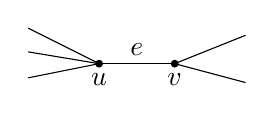
\begin{tikzpicture}
      [scale=.6]
      \coordinate (A) at (0, 0);
      \coordinate (B) at (1.6, 0);
      \coordinate (C) at (-1.5, 0.75);
      \coordinate (D) at (-1.5, 0.25);
      \coordinate (E) at (-1.5, -0.3);
      \coordinate (F) at (3.1, 0.6);
      \coordinate (G) at (3.1, -0.4);
      \foreach \from/\to in {A/B,A/C,A/D, A/E, B/F, B/G}
        \draw(\from) -- (\to);
        \filldraw[black] (A) circle (2pt)  node[below] {$u$};
        \filldraw[black] (B) circle (2pt)  node[below] {$v$};
        \node at (0.8,0.3) {$e$};
    \end{tikzpicture}
  }
  \qquad\quad
$G-e=$
  \parbox{1.02in}{   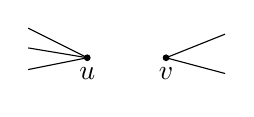
\begin{tikzpicture}
      [scale=.5]
      \coordinate (A) at (0, 0);
      \coordinate (B) at (2, 0);
      \coordinate (C) at (-1.5, 0.75);
      \coordinate (D) at (-1.5, 0.25);
      \coordinate (E) at (-1.5, -0.3);
      \coordinate (F) at (3.5, 0.6);
      \coordinate (G) at (3.5, -0.4);
      \foreach \from/\to in {A/C,A/D, A/E, B/F, B/G}
      \draw(\from) -- (\to);
      \filldraw[black] (A) circle (2pt)  node[below] {$u$};
      \filldraw[black] (B) circle (2pt)  node[below] {$v$};
    \end{tikzpicture}
}
\qquad\quad
$G_e=$
\parbox[c]{0.84in}{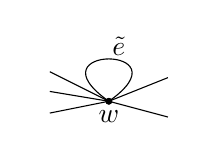
\begin{tikzpicture}
      [scale=.5]
      \coordinate (A) at (0, 0);
      \coordinate (C) at (-1.5, 0.75);
      \coordinate (D) at (-1.5, 0.25);
      \coordinate (E) at (-1.5, -0.3);
      \coordinate (F) at (1.5, 0.6);
      \coordinate (G) at (1.5, -0.4);
      \foreach \from/\to in {A/C,A/D, A/E, A/F, A/G}
      \draw(\from) -- (\to);
      \filldraw[black] (A) circle (2pt); % node[below] {\small 1};
      \node at (.25,1.4) {$\tilde{e}$};
      \draw (A) to[out=35,in=145,loop, min distance=2.5cm] (A);
      \filldraw[black] (A) circle (2pt)  node[below] {$w$};
    \end{tikzpicture}
   }
\caption{An edge $e=uv$ of $G$, the deletion $G-e$, and the contraction
$G_e$, in which $e$ becomes a loop $\widetilde e$ at the new vertex $w$.}
\label{fig:contraction}
\end{figure}


\subsection{Graph algebras, orientations, and functoriality}
\label{sec:graph-functoriality}
By an algebra in this paper we understand a commutative unital algebra over a fixed field $\K$ of characteristic $0$.

\begin{definition}
 Given a graph $G=(V,E)$, its \emph{edge algebra} $\Phi_G$ is the
 quotient of the polynomial algebra in \emph{edge variables}
 $\varphi_e, e\in E$, by their squares,
    \begin{equation}
    \label{eq:sq-free}
    \Phi_G:= \K[\varphi_e : e\in E]/(\varphi_e^2).
  \end{equation}
\end{definition}
The edge algebra is a local algebra of dimension $2^{|E|}$ isomorphic to the tensor product of $|E|$ copies of the algebra of dual numbers
$\K[\ve]/(\ve^2)$, namely
 \[
\Phi_G\simeq\bigotimes_{e\in E} \big(\K[\varphi_e]/(\varphi_e^2)\big).
 \]
%
It inherits the standard grading from the polynomial algebra. A basis of the $k$th graded component is given by square-free monomials of length $k$ in the edge variables $\varphi_e$. Each such monomial corresponds to a unique subset of $E$ which we can identify with a spanning subgraph of $G$.

The edge algebra has an unsigned contravariant functoriality,
independent of orientations. Every graph morphism~\eqref{eq:categ}
 \[
(\gamma,\lambda)\colon G\to G'
 \]
induces a natural homomorphism of algebras
 \[
\lambda^*\colon \Phi_{G'}\to \Phi_{G},
 \]
defined on generators
$\varphi_{e'}\in \Phi_{G'}$ by
\begin{equation}
  \label{eq:functor}
\lambda^*(\varphi_{e'}):=\sum_{e\in \lambda^{-1}(e')}\varphi_e.
\end{equation}
Thus, $\lambda^*(\varphi_{\lambda(e)})=\varphi_e$ and
$\lambda^*(\varphi_{e'})= 0$, if $e'\in E'$ is not in the image of $\lambda$.

\begin{definition}
Choose an orientation of each non-loop edge of $G=(V,E)$, independently
of the other edges. The \emph{zonotopal algebra} of $G$ is the subalgebra
$\CC_G$ of $\Phi_G$ generated by
\begin{equation}\label{eq:gens}
X_v=\sum_{e\in E}c_{v,e}\varphi_e,\qquad v\in V,
\end{equation}
where
\begin{equation}\label{eq:def}
c_{v,e}=\begin{cases}
 1,&e\text{ has tail }v\text{ and head different from }v,\\
 -1,&e\text{ has head }v\text{ and tail different from }v,\\
 0,&\text{otherwise, in particular if }e\text{ is a loop}.
\end{cases}
\end{equation}
A linear order on $V$ gives one possible orientation, from the smaller
to the larger endpoint, but no compatibility with a vertex order is
required.
\end{definition}

\begin{remark}\label{rem:orientations}
Orientations are suppressed in the notation $\CC_G$. If an orientation
$\omega'$ is obtained from $\omega$ by reversing some edges, let
$\eta_e=-1$ on those edges and $\eta_e=1$ on the other edges, including
loops. The graded automorphism
\[
\eta_G:\Phi_G\longrightarrow\Phi_G,\qquad
\varphi_e\longmapsto\eta_e\varphi_e,
\]
sends $X_v^\omega$ to $X_v^{\omega'}$. These reorientation maps compose
by multiplying their edge signs, and identify the corresponding
zonotopal algebras. Loop variables occur in none of the $X_v$; deleting
loops therefore leaves $\CC_G$ unchanged under the natural identification
inside the algebra on the remaining edge variables. We retain loops
because they arise under contraction.
\end{remark}

The unsigned map~\eqref{eq:functor} does not in general preserve the
zonotopal subalgebras. To define their functoriality, fix an orientation
for each graph and let $\phi=(\gamma,\lambda):G\to G'$ be a graph morphism.
If $e$ is oriented from $u$ to $v$ and $\lambda(e)$ is not a loop, set
$\varepsilon_\phi(e)=1$ when $\lambda(e)$ is oriented from $\gamma(u)$
to $\gamma(v)$, and $\varepsilon_\phi(e)=-1$ otherwise. If $\lambda(e)$
is a loop, set $\varepsilon_\phi(e)=1$; this includes every loop of $G$.
Define a signed homomorphism of edge algebras by
\begin{equation}\label{eq:signed-edge-pullback}
\phi^\sharp(\varphi_{e'})=
\begin{cases}
\varepsilon_\phi(e)\varphi_e,&e'=\lambda(e),\\
0,&e'\notin\lambda(E).
\end{cases}
\end{equation}
It is well-defined because $\lambda$ is injective and each image has
square zero.

\begin{proposition}[Signed pullbacks]\label{prop:graph-functor}
For every graph morphism $\phi=(\gamma,\lambda):G\to G'$, the restriction
of~\eqref{eq:signed-edge-pullback} gives a graded algebra homomorphism
$\phi^*:\CC_{G'}\to\CC_G$ satisfying
\begin{equation}\label{eq:vertex-pullback}
\phi^*(X_{v'}^{G'})=\sum_{v\in\gamma^{-1}(v')}X_v^G.
\end{equation}
These restrictions define a contravariant functor on $\cG$.
Changing the chosen orientations gives a naturally isomorphic functor
via the reorientation maps of Remark~\ref{rem:orientations}.
\end{proposition}
\begin{proof}
For every $e\in E$ and $v'\in V'$, the incidence coefficients satisfy
\[
\varepsilon_\phi(e)c^{G'}_{v',\lambda(e)}
=\sum_{v\in\gamma^{-1}(v')}c^G_{v,e}.
\]
For a non-loop image this is the definition of the sign. If $\lambda(e)$
is a loop, the left side is zero; on the right, either both endpoints
of a non-loop edge belong to the same fibre and their coefficients
cancel, or $e$ itself is a loop and both coefficients are zero.
This proves~\eqref{eq:vertex-pullback}, and hence preservation of the
subalgebras. Choices of signs on target loop variables do not affect
this restriction, since such variables do not occur in $\CC_{G'}$.
For a second graph morphism $\psi:G'\to G''$, applying the displayed
formula twice gives
\[
\phi^*\psi^*(X_{v''}^{G''})
=\sum_{v\in(\gamma_\psi\circ\gamma)^{-1}(v'')}X_v^G
=(\psi\circ\phi)^*(X_{v''}^{G''}).
\]
It also gives the identity map for the identity morphism. Since the
$X_v$ generate, this proves functoriality. The reorientation maps
commute with these restrictions by the same generator formula,
which proves the last assertion.
\end{proof}

\begin{remark}
If $\phi$ preserves the orientation of every edge with non-loop image,
then $\phi^\sharp$ is the unsigned map $\lambda^*$ of~\eqref{eq:functor}.
In general the chosen signed extensions $\phi^\sharp$ need not compose
on the full edge algebras: their composites can differ on a target
loop variable when an edge is collapsed. Functoriality holds for
the restrictions $\phi^*$, where these variables are absent. Thus the
unsigned edge-algebra functor and the zonotopal functor are distinct
constructions; no order-compatibility assumption is implicit.
\end{remark}

For deletion and contraction, choose the inherited orientation on every
edge that remains non-loop. For a non-loop edge $e=uv$, the graph $G_e$
of Figure~\ref{fig:contraction} retains $e$ as a loop $\widetilde e$, whereas $G/e$
is obtained by deleting that loop. Any other parallel edges become
loops as well. The chosen signed extension of $\pi_e:G\to G_e$ is then
the unsigned edge-bijection isomorphism $\Phi_{G_e}\to\Phi_G$.
Since loop variables do not occur in the incidence generators, its
restriction identifies $\CC_{G/e}$ with $\CC_{G_e}$ and gives an
injective homomorphism
\begin{equation}\label{eq:pi-emb}
\pi_e^*:\CC_{G/e}=\CC_{G_e}\longrightarrow\CC_G.
\end{equation}
It sends the generator at $w=\{u,v\}$ to $X_u+X_v$ and sends the
generator at any other vertex to the corresponding $X_p$. All
coefficients of edges between $u$ and $v$ cancel in $X_u+X_v$.
The image is therefore independent of the edge variables that become
loops, including $\varphi_e$.

\subsection{Presentation and deletion--contraction}
\label{sec:exact}

The deletion and contraction maps give the maps in the exact sequence
below. We use the inherited orientations throughout. Let $e\in E$ be a non-loop edge
with tail $u$ and head $v$.
Consider two algebra homomorphisms, the projection
\begin{equation}
  \label{eq:j-proj}
j_e^*\colon \CC_G\to \CC_{G-e},
\end{equation}
produced by sending $\varphi_e\in \Phi_G$ to $0$, and the embedding~\eqref{eq:pi-emb}
 \[
\pi_e^*\colon \CC_{G/e}=\CC_{G_e}\to \CC_G, \]
which maps $X_w$ to $X_u+X_v$.


Denote by
\begin{equation}
  \label{eq:derivative}
 \partial_e: = \frac{\partial}{\partial
   \varphi_e}\colon \Phi_G\to \Phi_G/(\varphi_e),
\end{equation}
the ``partial derivative'' with respect to the edge variable $\varphi_e\in \Phi_G$.
Modulo the ideal $(\varphi_e)$, the map $ \partial_e$ is well-defined.

The identification
   \[
  \Phi_G/(\varphi_e)\simeq \Phi_{G-e}
   \]
  endows $\Phi_{G-e}$ with a structure of a $\Phi_G$-algebra with respect to which  $\partial_e$ becomes a $\Phi_{G-e}$-valued derivation
   \[
  \delta_e\colon \Phi_G\to \Phi_{G-e}~.
   \]
For a reorientation map $\eta_G$ as in Remark~\ref{rem:orientations},
coefficient extraction satisfies
\[
\delta_e\circ\eta_G=\eta_e\,\eta_{G-e}\circ\delta_e.
\]
In particular, reversing $e$ changes this map by an overall sign under
the reorientation identifications. The contraction maps commute with
these identifications on the zonotopal algebras. Exactness and the
strictness assertions below are therefore independent of orientations.

To prove exactness without using a dimension formula, we will establish it
simultaneously with the power-algebra presentation, originally
established in~\cite{Wa1,PSS}.  For a graph $H$ and a subset $I\subseteq V(H)$,
let $D_I^H$ be the number of edges crossing the cut $I\mid V(H)-I$, and put
\[
R_H=\K[x_p:p\in V(H)],\qquad
\rho_I=\sum_{p\in I}x_p,\qquad
\mathcal I_H=(\rho_I^{D_I^H+1}:I\subseteq V(H)).
\]
The evaluation homomorphism
\[
\operatorname{ev}_H\colon R_H\longrightarrow\CC_H,\qquad x_p\longmapsto X_p,
\]
satisfies $\mathcal I_H\subseteq\ker\operatorname{ev}_H$: the element
$\rho_I(X)$ is a signed sum of the $D_I^H$ square-zero edge variables
crossing the cut.

For use also with the central quotient below, write
\begin{equation}\label{eq:two-power-ideals}
\mathcal I_H^{(\epsilon)}=
\left(\rho_{V(H)},\ \rho_I^{D_I^H+\epsilon}:
\varnothing\ne I\subsetneq V(H)\right),\qquad \epsilon\in\{0,1\}.
\end{equation}
Thus $\mathcal I_H^{(1)}=\mathcal I_H$. Exponent zero is allowed when
$\epsilon=0$, with the convention $\rho_I^0=1$. The relation
$\rho_{V(H)}$ is written separately in both cases.

\begin{lemma}[Cut-power antiderivatives]\label{lem:cut-antiderivative}
Let $e=uv$ be a non-loop edge of $G$, and set
$\mathcal D_e=\partial_{x_u}-\partial_{x_v}$ on $R_G=R_{G-e}$.
For $\epsilon=0,1$,
\begin{equation}\label{eq:cut-antiderivative}
\mathcal D_e(\mathcal I_G^{(\epsilon)})
=\mathcal I_{G-e}^{(\epsilon)}
\end{equation}
as vector subspaces of $R_G$. Every homogeneous element on the right of
degree $d$ has a homogeneous $\mathcal D_e$-antiderivative in the ideal
on the left of degree $d+1$.
\end{lemma}
\begin{proof}
For a proper nonempty subset $I\subseteq V$, put
$c_I=\mathcal D_e\rho_I\in\{0,1,-1\}$.
If $c_I=0$, then $D_I^G=D_I^{G-e}$ and $\rho_I$ is invariant.
If $c_I\ne0$, then $D_I^G=D_I^{G-e}+1$.
Differentiating any multiple of a generator of
$\mathcal I_G^{(\epsilon)}$ therefore gives an element of
$\mathcal I_{G-e}^{(\epsilon)}$. This also holds for the invariant
linear relation $\rho_V$.

Conversely, consider $\rho_I^Nq$ with $N=D_I^{G-e}+\epsilon$.
If $c_I=0$, choose $Q$ with $\mathcal D_eQ=q$ and use
$\mathcal D_e(\rho_I^NQ)=\rho_I^Nq$. Such a $Q$ exists because, in the
linear coordinates $x_u,x_u+x_v,x_p$ for $p\ne u,v$, the operator is
differentiation with respect to $x_u$.
If $c_I\ne0$, write
\[
R_G=(\ker\mathcal D_e)[\rho_I],\qquad
q=\sum_{j\ge0}q_j\rho_I^j,\qquad \mathcal D_eq_j=0.
\]
Then
\[
H=\frac1{c_I}\sum_{j\ge0}
\frac{q_j\rho_I^{N+j+1}}{N+j+1}
\]
satisfies $\mathcal D_eH=\rho_I^Nq$ and lies in
$(\rho_I^{N+1})\subseteq\mathcal I_G^{(\epsilon)}$.
Multiples of $\rho_V$ are integrated as in the invariant case.
These operations preserve homogeneity with degree increased by one.
There is no exception when $N=0$: in particular, a bridge cut in the
central case integrates the generator $1$ of the deletion ideal to
$\pm\rho_I$.
\end{proof}

For a graded algebra $A=\bigoplus_{k\ge0}A^{(k)}$, write
\begin{equation}\label{eq:hilbert}
H_A(t)=\sum_{k\ge0}\dim A^{(k)}t^k.
\end{equation}

\begin{theorem}[Presentation and deletion--contraction]
\label{th:graded-exact}
Let $G$ be a graph. Then:
\begin{enumerate}[(i)]
\item Evaluation $x_v\mapsto X_v$ induces a graded algebra isomorphism
\begin{equation}\label{eq:relF}
\CC_G\simeq \K[x_v:v\in V]/
\left(\left(\sum_{v\in I}x_v\right)^{D_I+1}:I\subseteq V\right),
\end{equation}
where $D_I$ is the number of edges crossing the cut $I\mid V-I$.
\item For every non-loop edge $e$, the derivation $\delta_e$ lowers degree
by one and the sequence of graded vector spaces
\begin{equation}\label{eq:exact}
0\longrightarrow\CC_{G/e}\xrightarrow{\pi_e^*}\CC_G
\xrightarrow{\delta_e}\CC_{G-e}[-1]\longrightarrow0
\end{equation}
is exact.
\item Consequently,
\begin{equation}\label{eq:Tutte}
H_{\CC_G}(t)=H_{\CC_{G/e}}(t)+tH_{\CC_{G-e}}(t).
\end{equation}
\end{enumerate}
\end{theorem}

\begin{proof}
We prove (i) and (ii) simultaneously by induction on the number of
non-loop edges; (iii) then follows by taking graded dimensions.
If there are no non-loop edges, every $X_p$ is zero and
$\mathcal I_G=(x_p:p\in V)$, so the presentation holds and there is
no exactness assertion to check. Otherwise, choose a non-loop edge
$e$ with tail $u$ and head $v$, and write $\overline X_p=j_e^*X_p$.
The action of $\delta_e$ on the generators~\eqref{eq:gens} is
\begin{equation}\label{eq:deriv}
\delta_e(X_p)=
\begin{cases}
  1,&p=u,\\
 -1,&p=v,\\
  0,&p\notin\{u,v\}.
\end{cases}
\end{equation}
Since $\delta_e$ is a $j_e^*$-derivation, formula~\eqref{eq:deriv} gives,
for every $F\in R_G$,
\begin{equation}\label{eq:polynomial-derivative}
\delta_e(F(X))=(\mathcal D_eF)(\overline X).
\end{equation}
This proves the assertion about degree. It also proves surjectivity: if $Q(\overline X)$ is an
element of $\CC_{G-e}$, choose a polynomial $F$ with
$\mathcal D_eF=Q$.  When $Q$ is homogeneous of degree $d$, the
antiderivative $F$ can be chosen homogeneous of degree $d+1$.
The map $\pi_e^*$ is injective by~\eqref{eq:pi-emb}, and its image is
annihilated by $\delta_e$.

It remains to prove exactness at $\CC_G$ and the presentation
\begin{equation}\label{eq:graded-presentation-kernel}
\ker\operatorname{ev}_G=\mathcal I_G.
\end{equation}
Assume the presentation is known for graphs with fewer non-loop edges.
Let $Z=F(X)\in\CC_G$ satisfy $\delta_eZ=0$.
By~\eqref{eq:polynomial-derivative} and the inductive hypothesis for
$G-e$, we have $\mathcal D_eF\in\mathcal I_{G-e}$.
Lemma~\ref{lem:cut-antiderivative} gives $H\in\mathcal I_G$ with
$\mathcal D_eH=\mathcal D_eF$.  Consequently
\[
P:=F-H\in\ker\mathcal D_e
 =\K[x_u+x_v,\,x_p:p\ne u,v].
\]
Since $H(X)=0$, we have $Z=P(X)$.  The evaluations of polynomials in
this last ring form precisely the image of $\pi_e^*$: the variable at
the contracted vertex $w$ maps to $X_u+X_v$, and the remaining variables
map to $X_p$, $p\ne u,v$.  This proves
$\ker\delta_e=\operatorname{im}\pi_e^*$.
All these constructions can be made homogeneously by the last assertion
of Lemma~\ref{lem:cut-antiderivative}, so exactness holds in every degree.

It remains to prove~\eqref{eq:graded-presentation-kernel} for $G$ and
thereby close the induction.  If $F(X)=0$, the same construction gives
$F=H+P$, with $H\in\mathcal I_G$ and $P\in\ker\mathcal D_e$.
Identify $R_{G/e}$ with $\ker\mathcal D_e$ by sending $x_w$ to
$x_u+x_v$.  The polynomial corresponding to $P$ evaluates to zero in
$\CC_{G/e}$, because its image $P(X)$ under the injective map $\pi_e^*$
is zero.  By the inductive hypothesis for $G/e$, it belongs to
$\mathcal I_{G/e}$.
Every generator of this ideal maps to a generator of $\mathcal I_G$:
a subset of $V(G/e)$ corresponds to a subset of $V(G)$ containing both
$u,v$, or neither, and the cut size is unchanged.  Hence
$P\in\mathcal I_G$, and therefore $F\in\mathcal I_G$.
This proves~\eqref{eq:graded-presentation-kernel} and completes the
induction.
\end{proof}

\begin{remark}[Bizonotopal algebras]\label{rem:bizonotopal}
Kirillov, Nenashev and the first and third authors use the same scheme
for the external bizonotopal algebra $\mathcal B_G$, generated by vertex
elements in the square-free algebra of the arrows of both orientations
of the edges \cite{KNSV}. A derivation and the embedding of the algebra
of the loopy contraction, which is the graph $G_e$ above, give an exact
sequence
$0\to\mathcal B_{G_e}\to\mathcal B_G\to\mathcal B_{G-e}[-1]\to0$
modeled on~\eqref{eq:exact} \cite[Proposition~3.7 and
Corollary~3.8]{KNSV}. The difference lies in the loops: they do not
contribute to $\CC_G$, so that $\CC_{G_e}=\CC_{G/e}$, whereas the loops
of $G_e$ contribute to $\mathcal B_{G_e}$. The Hilbert series therefore
satisfy the same relation as in~\eqref{eq:Tutte}, with $G_e$ in place of
$G/e$, but they are not specializations of the Tutte polynomial.
\end{remark}


\subsection{Spanning forests and Hilbert series}

The exact sequence~\eqref{eq:exact} gives the formulas for the dimension and the Hilbert series of $\CC_G$, first proved in~\cite{Wa1,PSS}.

A \emph{spanning forest} of $G=(V,E)$ is an acyclic spanning subgraph,
equivalently an acyclic subset of $E$. We recall external activity
before stating the Hilbert-series formula.

\begin{definition}
Let $G=(V,E)$ be a graph with some linear order on the set of edges $E$.
Let  $F\subset E$ be a spanning forest of $G$.
An edge $e\in E-F$ is called \emph{externally active} for $F$, if the subgraph $F\cup \{e\}$ contains a cycle and the edge $e$ is the smallest element of this cycle.

The number $\alpha(F)$ of externally active edges for $F$ is called the \emph{external activity} of $F$.
\end{definition}

Although $\alpha(F)$ depends on the edge order, the joint distribution
of $|F|$ and $\alpha(F)$ does not. More precisely, if
$r(G)=|V(G)|-c(G)$, where $c(G)$ is the number of connected components,
then
\[
 \sum_{F\text{ spanning forest of }G}
 z^{r(G)-|F|}w^{\alpha(F)}=T_G(1+z,w)
 \qquad\cite{Tut,Bjo}.
\]
The joint counts are therefore coefficients of a shifted Tutte polynomial.
The following theorem uses the coarser distribution of
$|E|-|F|-\alpha(F)$; it does not recover the two statistics separately.
Every loop is externally active for every forest, so $\alpha(F)$ is at
least the number of loops.


\begin{theorem}[\cite {PSS,Wa1}]
\label{th:forests}
Let $G=(V,E)$ be a graph.
\begin{enumerate}[(i)]
\item  The dimension of the algebra $\CC_G$ is equal to the number of spanning forests of $G$.

\item
  The dimension of the $k$th graded component $\CC_G^{(k)}$ of $\CC_G$ is
equal to the number of spanning forests $F\subseteq E$ with the external activity
 \[\alpha(F)=|E|-|F|-k. \]
\end{enumerate}
\end{theorem}

\begin{proof}
Since $\ds \dim \CC_G=\sum_{k\ge 0}\dim\CC_G^{(k)}$, part (i) follows from (ii).

Fix a linear order on $E$, and give every graph obtained from $G$ by deleting or contracting edges the induced order on its remaining edges. Let
$
a_k(G)=\bigl|\{F\subset E \,| \, \alpha(F)=|E|-|F|-k\}\bigr|
$
be the number of spanning forests of a graph $G$ with the external activity $|E|-|F|-k$, and let
 \[
F_G(t)=\sum_{k\ge 0} a_k(G)t^k
 \]
be its generating function. Then (ii) is equivalent to the equality
$H_{\CC_G}(t)=F_G(t)$. We prove this equality for every graph and every order, by induction on the number of non-loop edges.

If $G$ is a graph without non-loop edges, then it has only one spanning forest $F=\emptyset$ for which all edges (loops) are externally active. Thus $\alpha(F)=|E|=|E|-|F|$  and $F_G(t)=1$.
Since $H_{\CC_G}$ satisfies~\eqref{eq:Tutte} and the two series agree when $G$ has no non-loop edges, to prove (ii) it is sufficient, by induction on the number of non-loop edges, to show that $F_G$ satisfies the analogous deletion-contraction relation:
 \[
F_G(t)=F_{G/e}(t)+tF_{G-e}(t)
 \]
or, equivalently, that for every $G$ we have
\begin{equation}
  \label{eq:forests}
  a_k(G)=a_k(G/e)+a_{k-1}(G-e), \ k\ge 0.
\end{equation}
Denote by $\cF(G)$ the set of forests in a graph $G$.
If $e\in E$ is a non-loop edge, then $\cF(G)=\cF_+(G)\sqcup \cF_-(G)$,
where
 \[\cF_+(G)=\{F\in \cF(G) \,|\, e\in F\} \]
and
 \[\cF_-(G)=\{F\in \cF(G) \,|\, e\not\in F\}. \]
These subsets can be identified with the sets of forests $\cF(G/e)$ and $\cF(G-e)$ by the bijections
 \[
f_+\colon \cF(G/e) \to \cF_+(G), \ F\mapsto F\sqcup \{e\}
 \]
and
 \[
f_-\colon \cF(G-e) \to \cF_-(G), \ F\mapsto F.
 \]
To verify relation~\eqref{eq:forests}, we need to keep track of the numbers $a_k$. We do not reorder the edges: we take for $e$ the largest non-loop edge in the given order.
Then $\alpha(f_\pm(F))=\alpha(F)$ both for $F \in \cF(G/e)$ and $F \in \cF(G-e)$.  Indeed, let $e'\notin F\cup\{e\}$. If $e'$ is a loop of $G$, it is active on both sides. Otherwise the cycle of $F\cup\{e,e'\}$ in $G$, respectively of $F\cup\{e'\}$ in $G-e$, contains the non-loop edge $e'<e$, and contraction of $e$ identifies it with the cycle of $F\cup\{e'\}$ in $G/e$ after removing $e$; this does not change the smallest edge. Finally, $e$ itself is never externally active for $F\in\cF_-(G)$: a cycle through the non-loop edge $e$ contains another non-loop edge, which is smaller than $e$. In the first case, the term $|E|-|F|$ stays the same, so forests from $\cF(G/e)$ and $\cF_+(G)$ contribute to the same coefficient $a_k$. In the second case the difference $|E|-|F|$ changes by $1$, therefore forests from $\cF(G-e)$ contribute to $a_{k-1}$, as required.
Since the order was arbitrary and $H_{\CC_G}$ does not depend on it, this also proves that the numbers $a_k(G)$ are independent of the order.
\end{proof}


\subsection{Central algebras and spanning trees}
\label{sec:central}

The same antiderivative argument gives the central, or spanning-tree
counting, algebra of Postnikov and Shapiro. We include its presentation
and Hilbert formula to parallel the external theory above; see
\cite[Theorem~9.1 and Corollary~10.5]{PS} and
\cite[Section~4, Theorem~7]{NSh}. Filtered central algebras, generated
by the elements $f(X_v)$ in the quotient $\Phi_G^{\mathrm c}$ below, are
introduced in \cite[Section~4]{NSh}. They are not used in the subsequent
sections; see Section~\ref{sec:outlook}.

Let $G$ be a connected graph with nonempty vertex set. Define its
\emph{central zonotopal algebra} as the power quotient
\begin{equation}\label{eq:central-power-quotient}
\CC_G^{\mathrm c}=R_G/\mathcal I_G^{(0)}
=\K[x_v:v\in V]\big/
\left(\rho_V,\ \rho_I^{D_I}:\varnothing\ne I\subsetneq V\right).
\end{equation}
Eliminating one variable with $\rho_V=0$ gives the usual rooted
presentation. The full-set relation is linear, not $\rho_V^{D_V}=1$.
For the deletion--contraction induction we use the same quotient on a
disconnected graph. A proper union of connected components has cut size
zero, so this auxiliary quotient is zero. This is the spanning-tree
convention, not the tensor product of central algebras of the components.

To realize the quotient without using its dimension, set
\begin{equation}\label{eq:slim-edge-algebra}
\Phi_G^{\mathrm c}=
\Phi_G/(\varphi_S:G-S\text{ is disconnected}),\qquad
\varphi_S=\prod_{e\in S}\varphi_e.
\end{equation}
A set $S\subseteq E$ is called \emph{slim} when $G-S$ is connected.
The slim monomials form a basis of $\Phi_G^{\mathrm c}$.
For disconnected $G$, the empty support is nonslim and this algebra is
zero, consistently with the convention above. Write
$\widetilde{\CC}_G^{\mathrm c}$ for its subalgebra generated by the
incidence sums $X_v$.
Reorientation sign changes preserve the nonslim-monomial ideal, so
these incidence subalgebras are identified under reorientation as in
Remark~\ref{rem:orientations}. The deletion and contraction maps below
use inherited orientations. These sums satisfy $\sum_vX_v=0$ and,
for a proper cut of size $D_I>0$,
\[
\left(\sum_{v\in I}X_v\right)^{D_I}
=\pm D_I!\prod_{e\in\delta(I)}\varphi_e=0.
\]
Consequently evaluation induces a surjection
$\CC_G^{\mathrm c}\to\widetilde{\CC}_G^{\mathrm c}$.

\begin{lemma}[Slim deletion and contraction]\label{lem:slim-exact}
For every non-loop edge $e$, the inclusion of $e$-free monomials and
coefficient extraction induce an exact sequence of graded vector spaces
\begin{equation}\label{eq:slim-exact}
0\longrightarrow\Phi_{G/e}^{\mathrm c}
\xrightarrow{\iota_e}\Phi_G^{\mathrm c}
\xrightarrow{\delta_e}\Phi_{G-e}^{\mathrm c}[-1]
\longrightarrow0.
\end{equation}
The first map is an injective algebra homomorphism and sends the
contracted incidence generator to $X_u+X_v$.
\end{lemma}
\begin{proof}
For $S\subseteq E\setminus\{e\}$, the edge $e$ remains in $G-S$.
Contracting it does not change connectedness, so
\[
G-S\text{ connected}\quad\Longleftrightarrow\quad
(G/e)-S\text{ connected}.
\]
This identifies the $e$-free slim monomials with the basis on the left
of~\eqref{eq:slim-exact}. The slim monomials containing $e$ are
$\varphi_e\varphi_T$ with $(G-e)-T$ connected, and coefficient
extraction identifies them with the basis on the right.
With inherited orientations, the incidence formula for $\iota_e$
follows from cancellation at the endpoints of every edge joining
$u$ to $v$, including $e$; all other edge coefficients agree.
\end{proof}

Setting $\varphi_e=0$ also gives an algebra map
$j_e^*: \Phi_G^{\mathrm c}\to\Phi_{G-e}^{\mathrm c}$.
It need not identify $\Phi_G^{\mathrm c}/(\varphi_e)$ with
$\Phi_{G-e}^{\mathrm c}$: deletion can impose further nonslim-monomial
relations. Nevertheless $\delta_e$ is a $j_e^*$-derivation. In
particular, for $e$ oriented from $u$ to $v$,
\begin{equation}\label{eq:central-chain-rule}
\delta_e(F(X))=(\mathcal D_eF)(\overline X),\qquad
\overline X_p=j_e^*X_p.
\end{equation}

\begin{theorem}[Central presentation and deletion--contraction]
\label{thm:central-exact}
Evaluation identifies the power quotient~\eqref{eq:central-power-quotient}
with $\widetilde{\CC}_G^{\mathrm c}$. For every non-loop edge of a
connected graph, there is an exact sequence of graded vector spaces
\begin{equation}\label{eq:central-exact}
0\longrightarrow\CC_{G/e}^{\mathrm c}
\xrightarrow{\pi_e^*}\CC_G^{\mathrm c}
\xrightarrow{\delta_e}\CC_{G-e}^{\mathrm c}[-1]
\longrightarrow0,
\end{equation}
using the zero deletion term when $e$ is a bridge. Thus
\begin{equation}\label{eq:central-hilbert-rec}
H_{\CC_G^{\mathrm c}}(t)=
\begin{cases}
H_{\CC_{G/e}^{\mathrm c}}(t)+tH_{\CC_{G-e}^{\mathrm c}}(t),
 &e\text{ is not a bridge},\\
H_{\CC_{G/e}^{\mathrm c}}(t),&e\text{ is a bridge}.
\end{cases}
\end{equation}
Loops may be deleted without changing $\CC_G^{\mathrm c}$.
\end{theorem}
\begin{proof}
We prove the presentation and exactness simultaneously by induction on
the number of non-loop edges, as in Theorem~\ref{th:graded-exact}.
Disconnected graphs have both quotients zero. A connected graph without
non-loop edges has one vertex; its incidence algebra and its power
quotient are both $\K$, irrespective of its loops.

For a non-loop edge $e=uv$, Lemma~\ref{lem:slim-exact} gives an
injective contraction map on the incidence subalgebras.
Equation~\eqref{eq:central-chain-rule} gives surjectivity of $\delta_e$:
a polynomial representative $Q(\overline X)$ lifts by choosing
$F\in R_G$ with $\mathcal D_eF=Q$. The antiderivative may be chosen
homogeneous with degree raised by one.

If $F(X)\in\ker\delta_e$, the inductive presentation on $G-e$ gives
$\mathcal D_eF\in\mathcal I_{G-e}^{(0)}$.
Lemma~\ref{lem:cut-antiderivative}, with $\epsilon=0$, supplies
$H\in\mathcal I_G^{(0)}$ such that $\mathcal D_eH=\mathcal D_eF$.
Then
\[
P=F-H\in\ker\mathcal D_e
=\K[x_u+x_v,x_p:p\ne u,v].
\]
Since $H(X)=0$, the element $F(X)=P(X)$ belongs to the contraction
image. This proves exactness on the incidence subalgebras.

To close the induction, suppose $F(X)=0$. The same correction writes
$F=H+P$. Regard $P$ as a polynomial on $G/e$, substituting
$x_w=x_u+x_v$ at the contracted vertex. Its evaluation on $G/e$ is
zero because the ambient contraction map is injective. The inductive
presentation puts it in $\mathcal I_{G/e}^{(0)}$.
The total relation maps to $\rho_V$, and every proper cut of $G/e$
corresponds to a cut of $G$ containing both $u,v$ or neither, with the
same size. Hence its ideal maps into $\mathcal I_G^{(0)}$.
Thus $P$, and then $F$, belongs to $\mathcal I_G^{(0)}$, proving the
presentation. All corrections can be made homogeneously.
The Hilbert relation follows from exactness. Finally, loops occur in
neither the cut sizes nor the incidence generators.
\end{proof}

\begin{corollary}[Spanning-tree activity formula]\label{cor:central-activity}
For a connected graph $G$, with external activity $\alpha(T)$ defined
as above,
\begin{equation}\label{eq:central-activity}
H_{\CC_G^{\mathrm c}}(t)
=\sum_{T\text{ spanning tree of }G}
 t^{|E|-|V|+1-\alpha(T)}.
\end{equation}
In particular, $\dim\CC_G^{\mathrm c}$ is the number of spanning trees.
Equivalently, the series is $t^{|E|-|V|+1}T_G(1,t^{-1})$.
\end{corollary}
\begin{proof}
Choose the non-loop edge $e$ largest in the edge ordering. Trees
containing $e$ correspond to trees of $G/e$, with unchanged external
activity and unchanged exponent in~\eqref{eq:central-activity}.
Trees omitting $e$ correspond to trees of $G-e$, again with unchanged
activity, but with exponent increased by one when viewed in $G$.
If $e$ is a bridge, every spanning tree contains $e$, so there are no
trees omitting $e$; this matches the bridge case
of~\eqref{eq:central-hilbert-rec}. A loop is externally active for every
tree, so deleting it decreases both $|E|$ and the external activity by
one and leaves every exponent unchanged. The activity sum therefore satisfies
\eqref{eq:central-hilbert-rec} and has value $1$ on a one-vertex graph,
just as the Hilbert series. Induction proves the formula, and $t=1$
gives the dimension. The last expression is the spanning-tree activity
specialization of the Tutte polynomial.
\end{proof}

For example, a tree has central algebra $\K$, an $n$-cycle has central
Hilbert series $1+(n-1)t$, and two vertices joined by $m$ parallel edges
have central Hilbert series $1+t+\cdots+t^{m-1}$.
For a disconnected graph one may instead define a componentwise central
algebra by tensoring the connected ones. It counts spanning forests
with one tree per component, but then the bridge case must remain
separate; it is not the zero convention used in~\eqref{eq:central-exact}.

\subsection{Recovery of the graphical matroid}
\label{sec:matroid-reconstruction}

The following classification was proved by Wagner~\cite[Theorem~1.10]{Wa1} and Nenashev~\cite[Theorem~2.1]{N1}\cite{Ne}.
We give a proof in which the reconstruction is read directly from the
highest-degree multiplication. Write $G^\circ$ for the graph obtained
from $G$ by deleting all loops. Isolated vertices may also be discarded.

\begin{theorem}[Wagner--Nenashev]\label{th:wagner-nenashev}
For any two graphs $G_1,G_2$, the following are equivalent:
\begin{enumerate}[(i)]
\item $\CC_{G_1}$ and $\CC_{G_2}$ are isomorphic as $\K$-algebras;
\item $\CC_{G_1}$ and $\CC_{G_2}$ are isomorphic as graded $\K$-algebras;
\item the graphical matroids $M(G_1^\circ)$ and $M(G_2^\circ)$ are isomorphic.
\end{enumerate}
\end{theorem}

\begin{proof}
Loops do not occur in the generators $X_v$, so we may assume that the
graphs are loopless. Let $A=\CC_G$, let $N=|E(G)|>0$, and put
$W=A^{(1)}$. For $e\in E(G)$ let $\ell_e\in W^*$ be extraction of the
coefficient of $\varphi_e$. Each $\ell_e$ is nonzero. For every $x\in W$,
\begin{equation}\label{eq:top-power-product}
x^N=N!\left(\prod_{e\in E(G)}\ell_e(x)\right)
            \prod_{e\in E(G)}\varphi_e.
\end{equation}
Since $\K$ is infinite, there is an $x$ for which every $\ell_e(x)$ is
nonzero. Thus $A^{(N)}=\K\prod_e\varphi_e$ and $A^{(j)}=0$ for $j>N$.

Let $\mathfrak m$ be the maximal ideal of $A$. Since $A$ is generated
in degree one, $\mathfrak m^j=\bigoplus_{k\ge j}A^{(k)}$. In particular,
$N$ is determined intrinsically by $\mathfrak m^{N+1}=0\ne\mathfrak m^N$,
and the homogeneous polynomial map
\[
\mathfrak m/\mathfrak m^2\longrightarrow\mathfrak m^N,
\qquad \overline x\longmapsto x^N
\]
is well-defined: changing $x$ by an element of $\mathfrak m^2$ changes
$x^N$ by an element of $\mathfrak m^{N+1}=0$.
After choosing an identification of the one-dimensional target with
$\K$, it is a polynomial $Q_A$ on $\mathfrak m/\mathfrak m^2\simeq W$,
well-defined up to scalar. Formula~\eqref{eq:top-power-product} gives
\[
Q_A\doteq\prod_{e\in E(G)}\ell_e,
\]
where $\doteq$ means equality up to a nonzero scalar.
Unique factorization recovers the multiset of lines
$\{\K\ell_e:e\in E(G)\}\subset\P(W^*)$, including repeated factors.
In vertex-potential coordinates these forms are $a_u-a_v$ for the
oriented edges $uv$, on the space of potentials modulo functions constant
on connected components. Their dependence matroid is $M(G)$.
An arbitrary algebra isomorphism preserves $Q_A$ up to a linear change of
variables and a scalar. This proves (i)$\Rightarrow$(iii).
If $N=0$, the algebra is $\K$ and the loopless matroid is empty, so the
same conclusion holds.

For (iii)$\Rightarrow$(ii), use Whitney's $2$-isomorphism theorem
\cite{Wh}: after disregarding isolated vertices, graphs with isomorphic
graphical matroids are related by identifications of vertices in distinct
components, their inverse cleavings, and twists at a two-vertex
separation. We check the induced cut spaces
$W_G=\Span\{X_v\}\subset\K^{E(G)}$.
Identification and cleaving leave this space unchanged, since additive
constants in vertex potentials can be chosen independently on the
components. For a twist with boundary vertices $u,v$, keep a potential
$a$ on the first side and replace it on the second side by
$a'_w=a_u+a_v-a_w$. This interchanges its boundary values and negates
all edge differences on the second side. Hence negating the edge
variables on that side maps the old cut space onto the new one.
These sign changes, and the signed edge permutations induced by
graph isomorphisms as in Proposition~\ref{prop:graph-functor}, extend
to graded isomorphisms of the square-zero edge algebras. They therefore identify the subalgebras generated by the cut
spaces. Finally, (ii)$\Rightarrow$(i) is immediate.
\end{proof}

\begin{remark}
The factorization argument also applies to a subalgebra of a square-zero
algebra generated by the rows of a matrix with no zero columns. Its
highest-power polynomial recovers the projective column configuration,
with multiplicities, not merely its dependence matroid. Conversely,
projectively equivalent configurations give isomorphic algebras by
permuting and rescaling the edge variables. Thus, within this class, the
highest-degree multiplication already determines the algebra. For graphs,
this is more information than the dimensions of the graded pieces, whose
Hilbert series is only a specialization of the Tutte polynomial.
\end{remark}

The next section changes the filtration while retaining the underlying
algebra. For loopless graphs without isolated vertices, multiple edges
allowed, a nonzero quadratic coefficient makes this filtered invariant
complete (Theorem~\ref{th:Isom-f}).


\section{Polynomially generated filtrations}
\label{sec:prel}

\subsection{Definition and general properties}
\label{sec:def-filt}

We apply a power series to the vertex generators and filter the resulting
subalgebra by the number of factors. For nondegenerate series this is a
filtration of the fixed algebra $\CC_G$; degenerate series may generate
a smaller algebra. The notation $\CC_G^f$ includes both the subalgebra
and its word filtration.

\begin{definition}
  A formal power series
   \[f=a_0+a_1u+a_2u^2+\cdots \in \K[[u]] \]
is called  \emph{nondegenerate} if $a_1\ne 0$, i.e.\ when $f'(0)\ne 0$,
and \emph{degenerate} otherwise.
\end{definition}

\begin{definition}
  Let $G=(V,E)$ be a graph and let $f\in \K[[u]]$ be
  a power series.
The \emph{filtered external zonotopal algebra} of $G$ associated to $f$
is the subalgebra $\CC_G^f$ of $\Phi_G$~\eqref{eq:sq-free}, with its
filtration by degree in the generators
\begin{equation}
  \label{eq:gensY}
Y_v:=f(X_v)=f\Bigl(\sum_{e\in E} c_{v,e}\varphi_e\Bigr), \ v\in V,
\end{equation}
where the coefficients $c_{v,e}\in \{0,\pm 1\}$ are given by~\eqref{eq:def}.
\end{definition}
For nondegenerate $f$ the algebra $\CC^f_G$ is all of $\CC_G$
(Proposition~\ref{prop:same-algebra}); for degenerate $f$ it is in
general a proper subalgebra (Section~\ref{sec:degenerate}).
If $f=u$, then  $\CC^f_G$ is the usual zonotopal algebra  $\CC_G$ of $G$,  and if  $f=e^u$,  the filtered algebra $\CC^f_G$  is the $K$-theoretic analog $\cK_G$ of $\CC_G$ studied in \cite{NSh}.
\begin{remark}
\label{rem:nilpot}
The generators  $Y_v=f(X_v)$ are well-defined because $\varphi_e^2=0$ implies that
\begin{equation}
  \label{eq:nilpot}
  X_v^m=\Bigl( \sum_{e\in E} c_{v,e}\varphi_e \Bigr)^m=0,  \text{ for } m>\deg v
\end{equation}
   and so the power series~\eqref{eq:gensY} terminates.
   This also shows that the terms of $f$ of degree higher than
   \[ \Delta(G):=\max_{v\in V}\deg v
   \]
do not affect any of the generators $Y_v$ of $\CC_G^f$.
%
Therefore, we may restrict our attention to those $f\in \K[[u]]$ which are polynomials in $u$ of degree at most $\Delta(G)$.
\end{remark}


The algebra $\CC^f_G$ is endowed with an increasing filtration
\begin{equation}
  \label{eq:filtration}
\K=\CC^{f,0}_G\subset\CC^{f,1}_G\subset\CC^{f,2}_G\subset\cdots \subset \CC^f_G,
\end{equation}
where the subspace $\CC^{f,i}_G$ is spanned by the monomials of degree at most $i$ in the generators $Y_v=f(X_v)$.

\begin{remark}
\label{rem:const}
Replacing $f$ by $f+c$ with $c\in\K=\CC^{f,0}_G$ changes each $Y_v$ to
$Y_v+c$, and multiplying $f$ by a nonzero scalar rescales the $Y_v$.
Neither changes the filtration~\eqref{eq:filtration}. For nondegenerate
$f$ we therefore assume from now on that $f\equiv u\pmod{u^2}$;
degenerate $f$ are treated in Section~\ref{sec:degenerate}.
\end{remark}

When $f = u$, the filtration~\eqref{eq:filtration} coincides with the filtration induced on  $\CC_G$ by its standard grading.

\begin{remark}[Functoriality]\label{rem:filtered-functoriality}
Reorientation preserves these filtrations, since
$\eta_G(f(X_v^\omega))=f(X_v^{\omega'})$; the maps of
Remark~\ref{rem:orientations} are filtered algebra isomorphisms.
For a graph morphism $\phi=(\gamma,\lambda)$,
\begin{equation}\label{eq:filtered-vertex-pullback}
\phi^*(Y_{v'}^{G'})=
 f\left(\sum_{v\in\gamma^{-1}(v')}X_v^G\right).
\end{equation}
After subtracting $f(0)$, which does not change the filtration, the
images for injective $\gamma$ are the $Y_v^G$ and zeros. Thus
$\phi^*(\CC_{G'}^{f,i})=\CC_G^{f,i}$ for all $i$. In particular, graph
isomorphisms induce filtered isomorphisms. When vertices are identified,
the right side of~\eqref{eq:filtered-vertex-pullback} need not lie in
the first filtered space; this is why filtered contraction is treated
separately in Section~\ref{sec:filtered-exact}.
\end{remark}


Nondegenerate functions give filtrations of one fixed algebra. Degenerate
functions, treated in Section~\ref{sec:degenerate}, need not do so.

\begin{proposition}[{\cite[Proposition~2]{NSh}}]
\label{prop:same-algebra}
If $f\in \K[[u]]$ is a nondegenerate series, then $\CC^f_G$  coincides, as a subalgebra of $\Phi_G$, with the usual zonotopal algebra $\CC_G$.
\end{proposition}


\begin{proof}
After subtracting the constant term, write
$f(u)=c_1u+c_2u^2+\cdots$, with $c_1\ne0$. Each $Y_v=f(X_v)$ belongs
to $\CC_G$, so $\CC_G^f\subseteq\CC_G$. The formal compositional
inverse $g$ exists: its coefficients are determined successively by
$g(f(u))=u$, since the coefficient of the next unknown is a nonzero
power of $c_1$. Truncating $g$ after degree $\Delta(G)$ gives
$g(f(X_v))=X_v$ for every vertex. Thus every $X_v$ belongs to
$\CC_G^f$, proving the reverse inclusion.
\end{proof}


The increasing word filtration varies with $f$. By contrast, the
decreasing filtration by powers of the maximal ideal recovers the
original graded algebra. These are different filtrations on the same
underlying algebra.


\begin{corollary}\label{cor:assoc-graded}
Let $f\in u\K[[u]]$ be a nondegenerate series and let $J$ be the ideal of the algebra $\CC_G^f$ generated by the elements $Y_v=f(X_v)$, $v\in V$.
Then the associated graded algebra $\gr_J(\CC_G^f)$ for the $J$-adic filtration
\[
\CC_G^f\supset J\supset J^2\supset \cdots \supset  0
\]
is isomorphic to the graded algebra $\CC_G$.
\end{corollary}
\begin{proof}
By Proposition~\ref{prop:same-algebra}, $\CC^f_G=\CC_G$ as algebras.  The algebra $\CC_G$ is local: it is the direct sum of $\K$ and its ideal $\mathfrak m$ of elements without constant term, and $\mathfrak m$ is nilpotent.  Since $\CC_G$ is generated by the elements $X_v$, the ideal $\mathfrak m$ is generated by them; moreover, $Y_v=f(X_v)=X_v\cdot u_v$, where $u_v=a_1+a_2X_v+\cdots$ is a unit of $\CC_G$ ($a_1\ne0$ by nondegeneracy), so $J=(Y_v : v\in V)=(X_v : v\in V)=\mathfrak m$.  Finally, since the graded algebra $\CC_G$ is generated in degree one, $\mathfrak m^k=\bigoplus_{j\ge k}\CC_G^{(j)}$, whence
\[
\gr_J(\CC^f_G)=\bigoplus_{k\ge0}\mathfrak m^k/\mathfrak m^{k+1}\cong\bigoplus_{k\ge0}\CC_G^{(k)}=\CC_G.
\qedhere
\]
\end{proof}


\subsection{Recovery of the graph from its filtration}
\label{sec:filtered-reconstruction}

The following result concerns filtered isomorphism types, rather than
Hilbert functions. It applies to every $f$ with nonzero quadratic
coefficient, not just to a generic parameter.

\begin{theorem}
\label{th:Isom-f}
Let $f$ be a polynomial with nonzero linear and quadratic terms and let
$G_1$ and $G_2$ be two loopless graphs without isolated vertices; multiple
edges are allowed.
Then  $\CC^f_{G_1}$ and $\CC^f_{G_2}$ are isomorphic as filtered algebras  if and  only if  the graphs $G_1$ and $G_2$ are isomorphic.
\end{theorem}

For simple graphs this is \cite[Theorem~6]{NSh}, and for $f=e^u-1$ it is
\cite[Theorem~5]{NSh}. Loops and isolated vertices do not occur in the
generators $f(X_v)$. Hence, for arbitrary graphs, the filtered algebra
determines the graph obtained by deleting all loops and isolated
vertices, and nothing more.

\begin{proof}
The implication from graph isomorphism follows from the signed
pullback of Proposition~\ref{prop:graph-functor} and
\eqref{eq:filtered-vertex-pullback}. Conversely, let
$\Psi:\CC_H^f\longrightarrow\CC_G^f$ be a filtered algebra isomorphism.
By the normalization in Remark~\ref{rem:const}, write
$f(u)=u+\alpha u^2+\cdots$ with $\alpha\ne0$.
We use the edge configuration reconstructed in the proof of
Theorem~\ref{th:wagner-nenashev}, rather than reconstruct it a second time.

Put $W_G=\mathfrak m_G/\mathfrak m_G^2$ and define $W_H$ similarly.
The highest nonzero maximal-ideal power has degree
$N=|E(G)|=|E(H)|$ and is one-dimensional. The intrinsic highest-power
polynomial on $W_G$ factors as $Q_G\doteq\prod_e\ell_e$, where
$\ell_e$ extracts the coefficient of $\varphi_e$ in ordinary degree
one. Two edges $e,d$ give proportional forms if and only if they are
parallel: parallel edges give $\ell_d=\pm\ell_e$, and if $u$ is an
endpoint of $e$ but not of $d$, then $\ell_e(X_u)=\pm1$ while
$\ell_d(X_u)=0$. Here we use that the graphs are loopless. Thus the
distinct lines $\K\ell_e$ are indexed by the parallel classes of edges,
and the multiplicity of a line in $Q_G$ is the size of its class.
Let $G^{\mathrm s}$ be the simple graph obtained from $G$ by keeping one
edge from each parallel class, and let $m(e)$ be the size of the class
of $e$. Unique factorization applied to the linear map
$\overline\Psi:W_H\to W_G$ therefore gives a bijection
$\tau:E(G^{\mathrm s})\to E(H^{\mathrm s})$ with $m(\tau(e))=m(e)$, and
nonzero scalars $s_e$ such that
\begin{equation}\label{eq:filtered-edge-matching}
\ell_e\circ\overline\Psi=s_e\ell'_{\tau(e)}.
\end{equation}
The bijection preserves linear dependences, and hence the cycle
matroid of $G^{\mathrm s}$, including its three-edge circuits, which
are the triangles. If $N=0$, both graphs are empty because isolated
vertices are excluded, and there is nothing to prove.

Let $Z_w=\Psi(f(X_w^H))$. Since $Z_w$ is nilpotent and belongs to the
first filtered space, it is a linear combination of the $f(X_v^G)$,
with no constant term. Equation~\eqref{eq:filtered-edge-matching} gives
\[
[\varphi_e]Z_w=s_ec^H_{w,\tau(e)}.
\]
For $g=f^{-1}=u-\alpha u^2+\cdots$, the global incidence relation
on $H$ gives $\sum_wg(Z_w)=0$.
Take two disjoint edges $e,d$ of $G^{\mathrm s}$. No $f(X_v^G)$ contains the
monomial $\varphi_e\varphi_d$, because its support uses only edges
incident to $v$. Thus no $Z_w$ contains that monomial either.
Taking its coefficient in the inverse relation yields
\begin{equation}\label{eq:filtered-incidence-test}
0=-2\alpha s_es_d
\sum_{w\in V(H)}c^H_{w,\tau(e)}c^H_{w,\tau(d)}.
\end{equation}
The edges $\tau(e),\tau(d)$ are not parallel, so they share at most one
vertex. The sum is zero when they are disjoint and is $1$ or $-1$ when
they share a vertex. Thus $\tau(e),\tau(d)$ are disjoint. Applying the same argument to
$\Psi^{-1}$ proves the converse. The bijection therefore preserves
edge adjacency as well as triangles.

These data reconstruct the simple graph $G^{\mathrm s}$, which has no
isolated vertices.
Indeed, its stars at vertices of degree at least two are exactly the
maximal sets of at least two pairwise incident edges containing no
three-edge circuit. To check this, choose two edges with common
vertex $v$. Any edge meeting both either contains $v$ or completes
a triangle with them; the latter possibility is excluded.
Maximality then gives the full star at $v$. Create a vertex for each
such star. An edge belongs to zero, one, or two recovered stars; add
respectively two, one, or no leaf endpoints. The zero-star case is
an isolated $K_2$ component. This recovers all vertices and incidences,
so $\tau$ is induced by an isomorphism $G^{\mathrm s}\simeq H^{\mathrm s}$.
Since $\tau$ preserves the multiplicities $m$, this isomorphism extends
to an isomorphism $G\simeq H$.

The argument uses no extension of $\Psi$ to an ambient edge algebra
and no preservation of the original grading. Its linear data come
from $\mathfrak m/\mathfrak m^2$, and its quadratic test comes from
the actual first filtered space.
\end{proof}


\medskip

If the quadratic term of the polynomial $f(u)$ vanishes, the corresponding algebras for non-isomorphic graphs  can be isomorphic even as filtered algebras, as the following example shows.

\begin{proposition}
  \label{prop:D6E6}
Consider the trees $G_1=\mathrm D_6$ and $G_2=\mathrm E_6$ shown in Figure~\ref{fig:D6E6}, and let $f(u)=u+u^3$.
Then the filtered external zonotopal algebras $\CC^f_{G_1}$ and $\CC^f_{G_2}$ are isomorphic as filtered algebras.
\end{proposition}


\begin{figure}[htbp]
\centering
$G_1=$ \begin{minipage}[c]{5.0cm}
  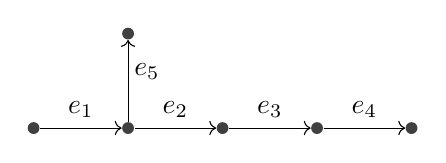
\begin{tikzpicture}
  [scale=1.2, auto=left, every node/.style={circle, fill=black!75,
    inner sep=0pt, minimum size=.15cm}]
    \node (n1) at (0,0) {};
    \node (n2) at (1,0) {};
    \node (n4) at (2,0) {};
    \node (n5) at (3,0) {};
    \node (n6) at (4,0) {};
    \node (n7) at (1,1) {};
    \foreach \from/\to in {n1/n2,n2/n4,n4/n5, n5/n6, n2/n7}
       \draw [->] (\from) -- (\to);
    \node[fill=white] at (.5,.2){$e_1$};
    \node[fill=white] at (1.5,.2){$e_2$};
    \node[fill=white] at (2.5,.2){$e_3$};
    \node[fill=white] at (3.5,.2){$e_4$};
    \node[fill=white] at (1.2,.6){$e_5$};
  \end{tikzpicture}
\end{minipage}
\qquad\qquad
$G_2=$
\begin{minipage}[c]{5.6cm}
  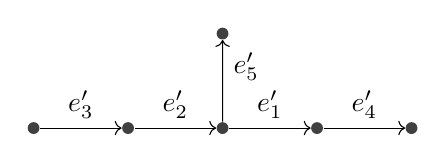
\begin{tikzpicture}
    [scale=1.2, auto=left, every node/.style={circle, fill=black!75,
      inner sep=0pt, minimum size=.15cm}]
    \node (n1) at (0,0) {};
    \node (n2) at (1,0) {};
    \node (n4) at (2,0) {};
    \node (n5) at (3,0) {};
    \node (n6) at (4,0) {};
    \node (n7) at (2,1) {};
    \foreach \from/\to in {n1/n2,n2/n4,n4/n5,n5/n6,n4/n7}
    \draw[->] (\from) -- (\to);
    \node[fill=white] at (.5,.25){$e'_3$};
    \node[fill=white] at (1.5,.25){$e'_2$};
    \node[fill=white] at (2.5,.25){$e'_1$};
    \node[fill=white] at (3.5,.25){$e'_4$};
    \node[fill=white] at (2.25,.65){$e'_5$};
\end{tikzpicture}
\end{minipage}
\caption{The trees $G_1=\mathrm D_6=T(1,1,3)$ and $G_2=\mathrm E_6=T(1,2,2)$ with the edge labels used in the proof of Proposition~\ref{prop:D6E6}. Their Hilbert series on the four subcubic cells are listed in Table~\ref{tab:D6E6}.}
\label{fig:D6E6}
\end{figure}


\begin{proof}
  Label the edges of the two graphs $e_1,\ldots,e_5,e'_1,\ldots,e_5'$ as shown in Figure~\ref{fig:D6E6} (notice the difference in placing the labels $e_1,e_3$ and $e_1',e_3'$) and denote by  $\varphi_1,\ldots,\varphi_5,\varphi_1',\ldots,\varphi_5'$ the corresponding generators of the edge algebras $\Phi_{G_1}$ and $\Phi_{G_2}$~\eqref{eq:sq-free}.
  The algebras $\CC^f_{G_1}$ and $\CC^f_{G_2}$ are the subalgebras of $\Phi_{G_1}$ and $\Phi_{G_2}$ generated, respectively,
  by $\{f(X_v)\}$  and $\{f(X_w)\}$, where $v\in  V(G_1)$, $w\in  V(G_2)$ and elements $X_v$ are given by~\eqref{eq:gens}.

  For $f=u+u^3$, since $\varphi_i^2=\varphi_i'^2=0$, we see that these sets of generators for $\CC_{G_1}^f$ and $\CC_{G_2}^f$ are, respectively, \[S_1=\{\varphi_1, -\varphi_1+\varphi_2+\varphi_5-6\varphi_1\varphi_2\varphi_5, \varphi_3-\varphi_2,\varphi_4-\varphi_3,-\varphi_4,-\varphi_5\}\]
and
\[S_2=\{\varphi_3', \varphi_2'-\varphi_3', \varphi'_1-\varphi'_2+\varphi'_5-6\varphi'_1\varphi'_2\varphi'_5, -\varphi'_1+\varphi'_4,-\varphi_4',-\varphi_5'\}.\]
The linear subspaces generated by these sets in $\Phi_{G_1}$ and $\Phi_{G_2}$
are, respectively,
$L_1=\langle S_1 \rangle=\langle \varphi_i,\varphi_1\varphi_2\varphi_5 \rangle$ and
$L_2=\langle S_2 \rangle=\langle \varphi'_i,\varphi'_1\varphi'_2\varphi'_5 \rangle$, $i=1,\ldots,5$.
Since the filtration~\eqref{eq:filtration} depends only on the linear span of the generating set (a product of at most $i$ elements of the span expands into products of at most $i$ generators, and vice versa), the isomorphism of algebras $\Phi_{G_1}\to \Phi_{G_2}$ sending $\varphi_i$ to $\varphi_i'$ maps $L_1$ onto $L_2$ and thus gives an isomorphism of the filtered algebras $\CC_{G_1}^f$ and $\CC_{G_2}^f$.

\end{proof}

\subsection{Generators and relations}
\label{sec:gen-rels}

Every element of the maximal ideal of $\Phi_G$ is nilpotent, so the
substitutions $a\mapsto f(a)$ and $a\mapsto f^{-1}(a)$ are defined on it
and are mutually inverse (Proposition~\ref{prop:same-algebra}). Hence
a polynomial relation $\rho(X_v:v\in V)=0$ holds in $\CC_G$ if and only
if $\rho(f^{-1}(Y_v):v\in V)=0$. Applied to the presentation of
Theorem~\ref{th:graded-exact}, this gives the relations among the
filtered generators.

\begin{corollary}\label{cor:relations}
  For a graph $G=(V,E)$ and a normalized nondegenerate $f \in \K[[u]]$,
consider the ideal
\begin{equation}
  \label{eq:relations}
I_G^f := \left(y_v^{\deg v+1}, \Bigl( \sum_{v\in I}f^{-1}(y_v) \Bigr) ^{D_I+1}\right)_{v\in V, \ I  \subseteq V, \ |I| \ge 2 }
\end{equation}
in \ $\K[y_v:v\in V]$, where $D_I$, as before, is the number of edges having one end in $I$ and the other  in the complementary subset $V-I$, and $\deg v=D_{\{v\}}$ is the number of non-loop edges at $v$.

Then $I_G^f$ is the ideal of relations for $\CC_G^f$, i.e.\ it is the kernel of the epimorphism
$\K[y_v \colon v\in V]\to \CC_G^f~.$
Therefore
\[\CC_G^f\simeq \K[y_v \colon v\in V]/I_G^f~.\]
 \end{corollary}
\begin{proof}
First quotient by $y_v^{\deg v+1}$ for all $v$. On this truncated
polynomial algebra, the substitutions $x_v=f^{-1}(y_v)$ and
$y_v=f(x_v)$ are mutually inverse automorphisms: the constant term of
$f$ is zero and its linear coefficient is nonzero. In particular,
$x_v^{\deg v+1}$ and $y_v^{\deg v+1}$ differ by a unit factor.
Under this change of variables, the remaining cut-power generators of
Theorem~\ref{th:graded-exact}(i) become exactly the displayed relations.
This proves both the presentation and that no further relations are
needed. In the displayed ideal, each $f^{-1}(y_v)$ may be truncated
modulo $y_v^{\deg v+1}$.
\end{proof}


\begin{remark}
Modulo the component-sum relation $\sum_{v\in V}f^{-1}(Y_v)=0$,
the cut sums for $I$ and $I^c$ are negatives of one another, and
$D_I=D_{I^c}$. Hence one relation from each complementary pair suffices;
keep the total-sum relation and all vertex nilpotence relations. For
example, choose the representative with smaller cardinality, breaking
ties arbitrarily. Section~\ref{sec:small-strata} gives examples of how
the remaining relations depend on the parameter.
\end{remark}

\subsection{Hilbert series}
\label{sec:alg}
We use the associated graded of the increasing word filtration to define
its Hilbert function, as in the Introduction. For a general filtered
vector space, the convention is the following.

\begin{definition}
  Let $W$ be a vector space with an exhaustive increasing filtration
\[ W^0 \subset W^1 \subset \cdots \subset W^i \subset \cdots \subset W
\]
 with $W^{-1}=0$, whose associated graded space
  \begin{equation}
    \label{eq:adj}
    \gr(W)=\bigoplus_{i\ge 0}W^i/W^{i-1}
  \end{equation}
  has finite-dimensional components $W^i/W^{i-1}$.

The sequence of integers
   \[ h_i(W)=\dim_\K W^i/W^{i-1} ,  \ i\ge 0,  \]
  is called the  \emph{Hilbert function} of $W$, and its generating function
  \begin{equation}
    \label{eq:hilb_series}
    \hs_W(t)=\sum_{i\ge 0}h_i(W)t^i
  \end{equation}
    is called the \emph{Hilbert series} of $W$.
  \end{definition}

The Hilbert functions and Hilbert series of  filtered external zonotopal algebras have some simple properties.


\begin{proposition}
\label{prop:hilb}
Let $G=(V,E)$ and let $f$ be any polynomial or formal power series.
Write $\hs_G^f(t)=\sum_{i\ge0}h_it^i$.
Then
\begin{enumerate}[(i)]
\item $\hs_G^f(t)$ is a polynomial in $t$ of degree $d\le |E|$.
\item $\ds h_i\le \binom{|V|+i-1}{i}$ for all $i$; in particular $h_0=1$.
\item If $f$ has nonzero linear and quadratic terms and the loopless graph $G^\circ$ has no isolated vertices or isolated edges, then $h_1=|V|$.
\item If $G=G_1\sqcup G_2$ is a disjoint union of two graphs $G_1$ and $G_2$, then
  \begin{equation}
    \label{eq:factor}
    \hs_G^f(t)=\hs_{G_1}^f(t)\,\hs_{G_2}^f(t).
  \end{equation}
\end{enumerate}
\end{proposition}
 \begin{proof}
Subtract $f(0)$ using Remark~\ref{rem:const}. Then every generator $Y_v$ lies in the maximal ideal $\mathfrak m=(\varphi_e: e\in E)$ of $\Phi_G$.  A product of more than $|E|$ elements of $\mathfrak m$ vanishes, since every square-free monomial contains at most $|E|$ variables; hence $\CC^{f,i}_G=\CC^{f,|E|}_G$ for $i\ge|E|$, and $h_i=0$ for $i>|E|$, proving (i).

For (ii), the graded quotient $\CC^{f,i}_G/\CC^{f,i-1}_G$ is spanned by the images of the products of exactly $i$ generators, i.e.\ by the images of the degree-$i$ monomials in the $|V|$ elements $Y_v$; the number of such monomials is $\binom{|V|+i-1}{i}$.

For (iii), suppose $\sum_v c_vY_v\in\K$ for some scalars $c_v$.  Comparing the linear parts in the edge variables gives $\sum_vc_vX_v=0$, which forces $c_v$ to be constant on every connected component of $G$, say $c_v=c_C$ for $v\in C$.

Comparing the quadratic parts then gives $a_2\sum_C c_C\,Q_C=0$, where $Q_C=\sum_{v\in C}X_v^2$ and $a_2\ne0$ is the quadratic coefficient of $f$.  For every pair of distinct edges $e,e'$ sharing at least one vertex, the coefficient of $\varphi_e\varphi_{e'}$ in $Q_C$ equals $2\sum_{v\in e\cap e'}c_{v,e}c_{v,e'}$, which is $\pm2$ if the edges share one vertex and $\pm4$ if they are parallel; hence $Q_C\ne0$ unless the component $C$ is an isolated vertex or an isolated edge.  Since the $Q_C$ are supported on disjoint sets of variable pairs, all $c_C$ vanish, so the classes of $Y_v$, $v\in V$, in $\CC^{f,1}_G/\CC^{f,0}_G$ are linearly independent and $h_1=|V|$.

Finally, (iv) holds because $\Phi_{G_1\sqcup G_2}=\Phi_{G_1}\otimes\Phi_{G_2}$, the generators of $\CC^f_{G_1\sqcup G_2}$ are those of the two factors, and consequently $\CC^{f,i}_{G_1\sqcup G_2}=\sum_{j+k\le i}\CC^{f,j}_{G_1}\otimes\CC^{f,k}_{G_2}$; the Hilbert series of such a tensor product with the convolution filtration is the product of the Hilbert series.
 \end{proof}


The first Hilbert coefficient also distinguishes the two cases in
maximum degree two.

\begin{proposition}\label{prop:max-degree-two}
Let $G$ be a loopless graph of maximum degree at most two, and let
$f=u+\alpha u^2+\cdots$ be normalized and nondegenerate. Then
$\hs^f_G$ depends only on whether $\alpha=0$. If $G$ has a vertex of
degree two, the two series $\hs^u_G$ and $\hs^{u+u^2}_G$ are different.
\end{proposition}
\begin{proof}
Since $X_v^3=0$ for every vertex, $Y_v=X_v+\alpha X_v^2$, and scaling every edge variable by $\varepsilon\ne0$, and dividing the
generators by $\varepsilon$, replaces $\alpha$ by $\varepsilon\alpha$.
Thus all nonzero values of $\alpha$ give isomorphic filtered algebras. Let $c$ be the number of components of $G$ and
$c_0$ the number of those that are isolated vertices or isolated edges.
For $f=u$ the relations among the $X_v$ are spanned by the component sums,
so $h_1=|V|-c$. For $\alpha\ne0$, the proof of
Proposition~\ref{prop:hilb}(iii) shows that a relation
$\sum_vc_vY_v\in\K$ vanishes on every other component, so
$h_1=|V|-c_0$. A vertex of degree two lies in a component
that is neither an isolated vertex nor an isolated edge, so $c>c_0$.
\end{proof}

\subsection{Filtered deletion--contraction and strictness}
\label{sec:filtered-exact}

For the graded algebras, the deletion--contraction sequence computes
Hilbert series recursively. We now ask when it remains exact at each
filtration level. It does so under mild conditions at an endpoint of
degree at most two (Theorem~\ref{th:del-contr}), but not in general
(Section~\ref{sec:strictness-counterexample}). This failure is the
reason for the boundary states of Section~\ref{sec:proofs}.

The underlying deletion--contraction sequence remains exact for every
nondegenerate $f$, but its restriction to filtration spaces need not be
exact. The issue is strictness of the contraction embedding.
Let $e=uv$ be a non-loop edge and let $w$ be the contracted vertex.
In this subsection assume that the generators at these vertices are linear:
\begin{equation}\label{eq:endpoint-linearity}
f(X_u)=X_u,\qquad f(X_v)=X_v,\qquad f(X_w)=X_w.
\end{equation}
A sufficient condition is $f\equiv u\pmod{u^m}$ with
\begin{equation}\label{eq:degs}
m\ge\max(\deg u+\deg v-1,\deg u+1,\deg v+1).
\end{equation}
Indeed, the three relevant nilpotence orders are at most
$\deg u+1$, $\deg v+1$, and $\deg u+\deg v-1$, respectively.
The corresponding endpoint generators after deleting $e$ are then linear
as well, by applying $j_e^*$.

\begin{proposition}[The strictness defect]\label{prop:filtered-defect}
Under~\eqref{eq:endpoint-linearity}, put
\[
F_i=\CC_G^{f,i},\qquad B_i=\pi_e^*(\CC_{G/e}^{f,i}),\qquad
F_i''=\CC_{G-e}^{f,i}.
\]
Then
\begin{equation}\label{eq:filtered-surjection}
B_i\subseteq F_i\cap\ker\delta_e,\qquad
\delta_e(F_i)=F_{i-1}''.
\end{equation}
The nonnegative integers
\begin{equation}\label{eq:strictness-defect}
d_i=\dim\frac{F_i\cap\ker\delta_e}{B_i}
\end{equation}
vanish for sufficiently large $i$, and
\begin{equation}\label{eq:hilbert-defect}
\hs_G^f(t)-\hs_{G/e}^f(t)-t\hs_{G-e}^f(t)
=(1-t)\sum_{i\ge0}d_it^i.
\end{equation}
Thus the deletion--contraction identity holds if and only if $\pi_e^*$
is strict, that is, $\pi_e^*(\CC_{G/e})\cap F_i=B_i$ for every $i$.
\end{proposition}
\begin{proof}
Orient $e$ from $u$ to $v$ and put
$T=X_u=\varphi_e+a$, where $a=j_e^*X_u$.
The filtration $B_\bullet$ is generated by $X_u+X_v$ and $Y_p$, $p\ne u,v$;
all these elements are $\varphi_e$-free. Replacing $Y_v$ by $Y_u+Y_v$
gives
\[
F_i=\sum_{r\ge0}T^rB_{i-r},\qquad
F_i''=\sum_{r\ge0}a^rB_{i-r}.
\]
Since $\delta_eT=1$ and $\delta_e$ vanishes on $B_\bullet$, it lowers
filtration by one. A representative
$\overline Z=\sum_rb_ra^r\in F_{i-1}''$, with $b_r\in B_{i-1-r}$,
has the lift
\[
Z=\sum_{r\ge0}\frac{b_rT^{r+1}}{r+1}\in F_i,
\qquad \delta_eZ=\overline Z.
\]
This proves~\eqref{eq:filtered-surjection}.
By Theorem~\ref{th:graded-exact} and Proposition~\ref{prop:same-algebra},
$\ker\delta_e=\pi_e^*(\CC_{G/e})$ as unfiltered vector spaces.
The filtrations are exhaustive, so $d_i=0$ for large $i$.
Rank--nullity gives
$\dim F_i=\dim B_i+\dim F_{i-1}''+d_i$.
Taking successive differences proves~\eqref{eq:hilbert-defect}, including
the stated equivalence.
\end{proof}

\begin{theorem}[A leaf or bivalent endpoint]\label{th:del-contr}
Assume~\eqref{eq:endpoint-linearity}, and suppose that at least one
endpoint of $e$ is incident to at most two non-loop edges.
Then, for every $i$, the sequence of vector spaces
\begin{equation}\label{eq:filtered-exact}
0\longrightarrow\CC_{G/e}^{f,i}\xrightarrow{\pi_e^*}
\CC_G^{f,i}\xrightarrow{\delta_e}\CC_{G-e}^{f,i-1}
\longrightarrow0
\end{equation}
is exact. In particular,
\begin{equation}\label{eq:del-contr}
\hs_G^f(t)=\hs_{G/e}^f(t)+t\hs_{G-e}^f(t).
\end{equation}
\end{theorem}
\begin{proof}
Take $u$ to be the endpoint of degree at most two and use the notation
of the preceding proof. There is at most one other edge at $u$, so
$a^2=0$, $T^2=2\varphi_ea$, and $T^3=0$. Hence
\begin{equation}\label{eq:bivalent-filtrations}
F_i=B_i+TB_{i-1}+T^2B_{i-2},\qquad F_i''=B_i+aB_{i-1}.
\end{equation}
These sums need not be direct. If
$Z=b_0+Tb_1+T^2b_2\in\ker\delta_e$, then
$b_1+2ab_2=0$. Therefore
\[
Tb_1+T^2b_2=-2(\varphi_e+a)ab_2+2\varphi_eab_2=0,
\]
and $Z=b_0\in B_i$. Thus every $d_i$ vanishes, and the preceding
proposition proves the theorem.
\end{proof}

\begin{corollary}\label{cor:tail}
If $e$ is a leaf edge whose other endpoint has degree $d$, and
$f\equiv cu\pmod{u^{d+1}}$ for $c\in\K^*$, then
\begin{equation}\label{eq:leaf-hs}
\hs_{\CC_G^f}(t)=(1+t)\hs_{\CC_{G/e}^f}(t).
\end{equation}
\end{corollary}
\begin{proof}
Divide $f$ by $c$, which does not change the filtration, and take $u$
to be the leaf vertex. Then $a=0$ and
$F_i=B_i\oplus\varphi_eB_{i-1}$; the sum is direct because $B_i$ is
$\varphi_e$-free. Taking successive differences proves the formula.
\end{proof}

\subsection{An unbounded strictness obstruction}
\label{sec:strictness-counterexample}

\begin{proposition}[Unbounded failure of strictness with trivalent endpoints]
\label{prop:filtered-nonstrict}
For every $m\ge5$, there is a simple tree $G$ with an edge $e=uv$,
$\deg u=\deg v=3$, for which $f=u+u^m$ satisfies
\eqref{eq:degs} but the contraction embedding is not strict.
More precisely, with $F_i,B_i$ as above there is an element $q$ such that
\[
q\in F_{m+1}\cap\pi_e^*(\CC_{G/e}),\qquad
q\in B_{2m}\setminus B_{2m-1}.
\]
Thus the discrepancy between the intrinsic contraction filtration and
the induced filtration is unbounded, even with the two endpoint degrees
fixed. The corresponding Hilbert series fail~\eqref{eq:del-contr}.
\end{proposition}
\begin{proof}
Start with $e=uv$, attach $h_1,h_2$ to $u$ and $h_3,h_4$ to $v$,
and attach $m-1$ leaves to each $h_i$. The merged vertex has degree four,
so~\eqref{eq:degs} holds. There are $4m+2$ vertices and $4m+1$ edges.

Orient $e$ from $u$ to $v$, the four branch edges towards the $h_i$,
and the leaf edges away from the $h_i$.  Denote the corresponding
edge variables by $\varepsilon=\varphi_e$, $a_i$, and $b_{ij}$,
respectively, where $1\le i\le4$ and $1\le j\le m-1$.  Set
\[
p_i=m!\prod_{j=1}^{m-1}b_{ij},\qquad
x_i=a_i(1+p_i),\qquad z_i=x_ip_i.
\]
Since $p_i^2=0$, we have $a_i=x_i-z_i$.  The change from $a_i$ to
$x_i$, fixing $\varepsilon$ and the $b_{ij}$, is an automorphism of the
square-zero edge algebra, with inverse $a_i=x_i(1-p_i)$.
Thus square-free monomials in $\varepsilon,x_i,b_{ij}$ form a basis
of $\Phi_G$.

At $h_i$ one has
\[
X_{h_i}=-a_i+\sum_jb_{ij},\qquad
X_{h_i}^m=-a_ip_i,\qquad
Y_{h_i}=\sum_jb_{ij}-x_i.
\]
The leaf generators are $-b_{ij}$.  Put
\[
S=z_1+z_2+z_3+z_4,\qquad r=z_1+z_2,\qquad T=\varepsilon-r.
\]
The two remaining generators of $\CC_G^f$ are
\[
Y_u=x_1+x_2+T,\qquad Y_v=x_3+x_4-S-T,
\]
whereas the contracted generator is $Y_w=\sum_i x_i-S$.
Consequently, writing $F_i$ and $B_i$ as in
Proposition~\ref{prop:filtered-defect}, the two filtrations are generated
in degree one by
\begin{equation}\label{eq:counterexample-generators}
\begin{array}{ll}
F_\bullet:&x_i,\ b_{ij},\ S,\ T,\\
B_\bullet:&x_i,\ b_{ij},\ S.
\end{array}
\end{equation}
Indeed, each of these collections has the same linear span as the
corresponding set of vertex generators.

Consider $q=z_1z_2$.  It is $\varepsilon$-free, so $\delta_eq=0$.
Each $z_i=x_ip_i$ is a scalar multiple of a product of $m$ degree-one
generators of $B_\bullet$, and hence $r\in B_m$.
The relations $(T+r)^2=\varepsilon^2=0$ and $r^2=2q$ give
\begin{equation}\label{eq:counterexample-early}
q=-\tfrac12T^2-Tr\in F_{m+1}.
\end{equation}
We claim, however, that
\begin{equation}\label{eq:counterexample-late}
q\notin B_{2m-1}.
\end{equation}

Let $M=\Span\{z_i z_j:1\le i<j\le4\}$, and let
$\operatorname{pr}_M$ be the coordinate projection onto these six
rescaled square-free monomials in the variables $x_i,b_{ij}$.
Use the auxiliary grading $\deg_x x_i=1$ and $\deg_x b_{ij}=0$.
Then $\deg_x z_i=\deg_x S=1$, so a monomial in the generators of
$B_\bullet$ in~\eqref{eq:counterexample-generators} can contribute to
$M$ only if it contains exactly two factors from the collection
$\{x_i,S\}$, counted with multiplicity.

If both factors are $x$-variables, a contribution to $z_i z_j$
requires all $2m-2$ leaf-edge variables in the two corresponding groups,
and therefore a product of $2m$ generators.  Such a product does not
occur among the spanning monomials of $B_{2m-1}$.
If the factors are $x_i$ and $S$, the only monomial in the leaf-edge
variables giving a nonzero projection is $\prod_jb_{ij}$; its
projection is a scalar multiple of $z_iS$. If both factors are $S$,
multiplication by a nonconstant monomial in the leaf-edge variables
gives terms that are either zero or have zero projection onto $M$.
Finally, $S^2=\sum_i z_iS$.  It follows that
\[
\operatorname{pr}_M(B_{2m-1})
\subseteq\Span\{z_1S,z_2S,z_3S,z_4S\}.
\]
The linear functional
\[
\lambda\left(\sum_{i<j}c_{ij}z_i z_j\right)
=c_{12}+c_{34}-c_{13}-c_{24}
\]
vanishes on each $z_iS$ but has value $1$ on $q$.
This proves~\eqref{eq:counterexample-late}.
Notice also that $q\in B_{2m}$ by its explicit expression as a product
of $2m$ generators.

Since $m+1\le2m-1$, equations~\eqref{eq:counterexample-early}
and~\eqref{eq:counterexample-late} show that
\[
q\in\ker\delta_e\cap F_{m+1},\qquad q\notin B_{m+1}.
\]
Thus $d_{m+1}>0$, and~\eqref{eq:hilbert-defect} implies that the
Hilbert series do not satisfy~\eqref{eq:del-contr}.
The two endpoint degrees are $3$ for every $m\ge5$, so increasing a
lower bound on $m$ depending only on those two degrees cannot restore
the general assertion.
\end{proof}


The obstruction above shows that filtered deletion--contraction alone
does not control the attachment of graphs. The next section keeps two
filtrations at a cut edge and computes directly with their joint birth
degrees.


\subsection{Degenerate functions}
\label{sec:degenerate}

Let $f$ be degenerate. Every element of $\CC_G^f$ is a constant plus
terms of degree at least two in the $\varphi_e$, so $\CC_G^f$ is a proper
subalgebra of $\CC_G$ as soon as $G$ has a non-loop edge. These filtered
algebras are the algebras $F[f]_G$ of \cite[Section~3]{NSh}. Nenashev
and the first author asked for the combinatorial properties of their
Hilbert series and, in particular, for the dimension of $\CC_G^f$
\cite[Problem~4]{NSh}. We answer this question for forests and for
cycles. By Remark~\ref{rem:const}, subtracting the constant term does not
change the filtration. A nonzero series with $f(0)=0$ has
\emph{order} $k$ if $f=cu^k+\text{terms of higher degree}$ with
$c\ne0$. It is degenerate exactly when $k\ge2$ and for $f=0$ the algebra is $\K$. Loops occur in
none of the $X_v$, so in this section all graphs are loopless.

\begin{definition}\label{def:partial-score}
A \emph{partial orientation} of a graph $G=(V,E)$ is a choice of
orientations for the edges of a subset $S\subseteq E$
\cite[Definition~2.1]{KNSV}. For $e\in S$ let $s(e)$ be the vertex at
which $e$ starts. The \emph{score vector} of the partial orientation is
$a\in\Z_{\ge0}^V$, where $a_v$ is the number of edges of $S$ starting at
$v$. The score vectors of partial orientations are the \emph{partial
score vectors} of $G$ \cite[Definition~2.4]{KNSV}. For $k\ge1$ put
\[
 s_k(G;t)=\sum_a t^{|a|/k},\qquad |a|=\sum_{v\in V}a_v,
\]
the sum over the partial score vectors $a$ with $k\mid a_v$ for all
$v\in V$.
\end{definition}

Removing an edge from $S$ shows that lowering an entry of a partial score
vector gives a partial score vector. By \cite[Corollary~2.6]{KNSV},
$s_1(G;t)$ is the Hilbert series of the external bizonotopal algebra
(Remark~\ref{rem:bizonotopal}).

\begin{theorem}\label{thm:degenerate-forests}
Let $G$ be a forest, let $k\ge2$, and let $f\in\K[u]$ have order $k$.
Put
\[
 \begin{aligned}
 \mathcal E_{G,k}&=\{m\in\Z_{\ge0}^{V(G)}:km\text{ is a partial score vector of }G\},\\
 I_{G,k}&=(z^m:m\notin\mathcal E_{G,k})\subseteq\K[z_v:v\in V(G)].
 \end{aligned}
\]
Evaluation induces an isomorphism of filtered algebras
\begin{equation}\label{eq:degenerate-forest-presentation}
 \K[z_v:v\in V(G)]/I_{G,k}\ \xrightarrow{\ \sim\ }\ \CC_G^f,
 \qquad z_v\longmapsto f(X_v),
\end{equation}
where the quotient on the left has its standard degree filtration.
Consequently
\[
 \hs_G^f(t)=s_k(G;t),\qquad
 \CC_G^f\simeq\CC_G^{u^k}\quad\text{as filtered algebras}.
\]
In particular, the filtered isomorphism type depends only on $G$ and
$k$, and its dimension counts the partial score vectors with every
entry divisible by $k$.
\end{theorem}

\begin{example}\label{ex:degenerate-examples}
\leavevmode
\begin{enumerate}[(i)]
\item Let $G$ be the path with $N$ edges and let $k=2$. An even partial
score vector takes the value $2$ on a set of pairwise nonadjacent inner
vertices and $0$ elsewhere. Hence $[t^m]\,\hs_G^f=\binom{N-m}{m}$, and
$\dim\CC_G^f$ is the Fibonacci number $F_{N+1}$, with $F_0=0$, $F_1=1$ and
$F_j=F_{j-1}+F_{j-2}$.
\item For the star with $N$ leaves,
$\hs_{S_{N+1}}^f=1+t+\cdots+t^{\lfloor N/k\rfloor}$.
\item If $k>\Delta(G)$, then all $Y_v$ vanish and $\CC_G^f=\K$; this
holds for every graph.
\end{enumerate}
\end{example}

For $a\in\Z_{\ge0}^V$, expanding the powers with $\varphi_e^2=0$ gives
\begin{equation}\label{eq:power-products}
 \prod_{v\in V}X_v^{a_v}=\prod_{v\in V}a_v!\cdot
 \sum_{S}\Bigl(\prod_{e\in S}c_{s(e),e}\Bigr)\varphi_S,
 \qquad \varphi_S=\prod_{e\in S}\varphi_e,
\end{equation}
the sum over the partial orientations with score vector $a$. Indeed,
$X_v^{a_v}$ is $a_v!$ times the sum of the products of $a_v$ distinct
terms $c_{v,e}\varphi_e$. Choosing such a product for every $v$ amounts
to orienting the chosen edges away from $v$, and the product of the
choices vanishes unless all the chosen edges are distinct. In particular,
$\prod_vX_v^{a_v}=0$ unless $a$ is a partial score vector.

\begin{lemma}\label{lem:degenerate-upper}
Let $G$ be a graph and let $f\in\K[u]$ have order $k\ge1$. Then
$\CC_G^{f,d}$ is spanned by the products $\prod_vY_v^{m_v}$ with
$\sum_vm_v\le d$ for which $km$ is a partial score vector. In particular,
$\dim\CC_G^{f,d}\le\sum_{m\le d}[t^m]\,s_k(G;t)$.
\end{lemma}
\begin{proof}
Since $f(u)^{m_v}$ is divisible by $u^{km_v}$, the product
$\prod_vY_v^{m_v}$ is a linear combination of products $\prod_vX_v^{j_v}$
with $j_v\ge km_v$ for all $v$. If $km$ is not a partial score vector,
then neither is any such $j$, and all these products vanish
by~\eqref{eq:power-products}.
\end{proof}

For a vertex $v$ let $e_j(v)$ be the $j$th elementary symmetric
polynomial in the variables $\varphi_e$ of the edges at $v$, with
$e_0(v)=1$ and $e_j(v)=0$ for $j<0$, and put $P_a=\prod_ve_{a_v}(v)$.
Then $P_a=\sum_SN_a(S)\,\varphi_S$, where $N_a(S)\ge0$ is the number of
orientations of $S$ with score vector $a$. In particular, $P_a\ne0$ if
and only if $a$ is a partial score vector.

\begin{lemma}\label{lem:no-consecutive}
Let $G$ be a forest and, for each $v\in V$, let $A_v\subseteq\Z_{\ge0}$
be a set that contains no two consecutive integers. Then the nonzero
elements $P_a$ with $a\in\prod_vA_v$ are linearly independent.
\end{lemma}
\begin{proof}
We use induction on the number of edges. If there are none, only
$P_0=1$ occurs. Otherwise let $\ell$ be a leaf, let $e=\ell p$ be its
edge and let $G'=G-\ell$. Write $P'_b$ for the corresponding elements of
$\Phi_{G'}\subset\Phi_G$, $e'_j(p)$ for the elementary symmetric
polynomials at $p$ in $G'$, and $a'$ for the restriction of $a$ to
$V\setminus\{\ell\}$. If $P_a\ne0$, then $a_\ell\in\{0,1\}$, since $\ell$
has degree one. Since $A_\ell$ contains no two consecutive integers,
$a_\ell$ takes the same value for all $a$ under consideration, and
$a\mapsto a'$ is injective.

If $a_\ell=1$, then $P_a=\varphi_e\,P'_{a'}$, because $\varphi_e\,e_j(p)=\varphi_e\,e'_j(p)$.
Multiplication by $\varphi_e$ is injective on $\Phi_{G'}$, and the claim
follows from the induction hypothesis for $G'$ and the sets $A_v$,
$v\ne\ell$.

If $a_\ell=0$, then $e_{a_p}(p)=e'_{a_p}(p)+\varphi_e\,e'_{a_p-1}(p)$
gives
\[
 P_a=P'_{a'}+\varphi_e\,P'_{a'-\delta_p},
\]
where $\delta_p$ is the indicator vector of $p$. Since
$\Phi_G=\Phi_{G'}\oplus\varphi_e\Phi_{G'}$, a relation
$\sum_ac_aP_a=0$ splits into $\sum_ac_aP'_{a'}=0$ and
$\sum_ac_aP'_{a'-\delta_p}=0$. The vectors $a'$ lie in
$\prod_{v\ne\ell}A_v$, so by induction $c_a=0$ whenever
$P'_{a'}\ne0$. For the remaining $a$ we have
$P_a=\varphi_e\,P'_{a'-\delta_p}\ne0$. The vectors $a'-\delta_p$ are
distinct and lie in the product of the sets $A_v$, $v\ne\ell,p$, and
$\{x-1:x\in A_p,\ x\ge1\}$, which again contains no two consecutive
integers. By induction $c_a=0$ for these $a$ as well.
\end{proof}

The hypothesis is needed: for the path with two edges and $A_v=\Z_{\ge0}$,
eight elements $P_a$ are nonzero, in an algebra of dimension four.

\begin{proof}[Proof of Theorem~\ref{thm:degenerate-forests}]
Partial score feasibility is downward closed. Hence $\mathcal E_{G,k}$
is a finite order ideal, $I_{G,k}$ is a monomial ideal, and the residue
classes of $\{z^m:m\in\mathcal E_{G,k}\}$ form a basis of
$\K[z_v:v\in V(G)]/I_{G,k}$.
Lemma~\ref{lem:degenerate-upper} shows that every generator of
$I_{G,k}$ evaluates to zero. It remains to prove the independence of
the feasible products $\prod_vY_v^{m_v}$. A forest is bipartite; orient every edge from one class
$V_+$ of a bipartition to the other class $V_-$
(Remark~\ref{rem:filtered-functoriality}). Then $c_{v,e}=\pm1$ for
$v\in V_\pm$ and every edge $e$ at $v$, and~\eqref{eq:power-products}
becomes $\prod_vX_v^{a_v}=\pm\prod_va_v!\cdot P_a$. The component of
lowest degree in the $\varphi_e$ of $\prod_vY_v^{m_v}$ is
\[
 c^{\sum_vm_v}\prod_vX_v^{km_v}=\pm c^{\sum_vm_v}\prod_v(km_v)!\cdot P_{km}\ne0.
\]
Since $k\ge2$, the set $k\Z_{\ge0}$ contains no two consecutive integers,
and Lemma~\ref{lem:no-consecutive} shows that these lowest components are
linearly independent. Elements whose lowest components are linearly
independent are linearly independent: in a nontrivial relation, consider
the smallest degree of a lowest component with nonzero coefficient.
Hence evaluation modulo $I_{G,k}$ is injective as well as surjective.
It maps the span of the standard monomials of degree at most $d$ onto
$\CC_G^{f,d}$ for every $d$, proving the filtered isomorphism and its
Hilbert formula.
\end{proof}

\begin{remark}\label{rem:degenerate-grading}
The presentation gives $\CC_G^f$ a grading in which the $Y_v$ have
degree one. This grading need not agree with ordinary edge degree in
$\Phi_G$. The same proof permits a different function $f_v$ at each
vertex, of order $k_v\ge2$: the standard monomials are those for which
$(k_vm_v)_v$ is a partial score vector. Only the orders $k_v$ matter.
Indeed, apply Lemma~\ref{lem:no-consecutive} with $A_v=k_v\Z_{\ge0}$
to the lowest-degree components of the products.
\end{remark}

\begin{corollary}\label{cor:degenerate-bounds}
Let $G$ be a graph and let $f\in\K[u]$ have order $k\ge2$, with
coefficient $c$ of its lowest nonzero term. Then for all $d$
\[
 \dim\CC_G^{u^k,d}\le\dim\CC_G^{f,d}\le\sum_{m\le d}[t^m]\,s_k(G;t),
\]
with equality for forests.
\end{corollary}
\begin{proof}
The upper bound is Lemma~\ref{lem:degenerate-upper}. For $\lambda\ne0$
the automorphism $\varphi_e\mapsto\lambda\varphi_e$ of $\Phi_G$ maps
$\CC_G^{f,d}$ onto $\CC_G^{f_\lambda,d}$, where
$f_\lambda(u)=\lambda^{-k}f(\lambda u)$. The coefficients of $f_\lambda$
are polynomials in $\lambda$, and $f_0=cu^k$. Ranks can only drop under
specialization, so
$\dim\CC_G^{u^k,d}=\dim\CC_G^{f_0,d}\le\dim\CC_G^{f_\lambda,d}=\dim\CC_G^{f,d}$.
\end{proof}

\begin{remark}\label{rem:degenerate-bizonotopal}
An orientation of $G$ defines a homomorphism from the partial orientation
algebra of \cite{KNSV} onto $\Phi_G$ that maps the external bizonotopal
algebra $\mathcal B_G$ onto $\CC_G$ and its generators $y_v$ to $X_v$
\cite[Section~2]{KNSV}. The monomials $y^a=\prod_vy_v^{a_v}$ for partial
score vectors $a$ form a basis of $\mathcal B_G$
\cite[Proposition~2.5]{KNSV}. Hence the subalgebra generated by the
$y_v^k$ has the basis $\{y^a:k\mid a\}$, and it maps onto $\CC_G^{u^k}$.
Theorem~\ref{thm:degenerate-forests} says that for a forest and $k\ge2$
this map is injective. For $k=1$ and a forest with at least one edge, it is not injective:
$\dim\mathcal B_G$ is the
number of partial score vectors and $\dim\CC_G$ is the number of spanning
forests. For an edgeless forest both algebras are $\K$.
\end{remark}

\begin{remark}\label{rem:degenerate-recursion}
For a tree, $s_k$ can be computed without listing score vectors. Root
the tree, and for a vertex $v$ with parent edge $g$ consider the vectors
on the subtree below $v$ with all entries divisible by $k$. Call such a
vector of the \emph{first kind} if it is the score vector of a partial
orientation of the subtree, and of the \emph{second kind} if it is not,
but becomes one when $g$ is added and oriented away from $v$. Let
$A_v(t)$ and $B_v(t)$ count the vectors of the two kinds with weight
$t^{|a|/k}$. Suppose that the restrictions of a vector to the subtrees of
the children of $v$ are of the two kinds, $j$ of them of the first kind.
The edge to a child of the second kind must start at that child, and the
edge to a child of the first kind may start at $v$. Hence the vector is
of the first kind if $a_v\le j$ and of the second kind if $a_v=j+1$.
With $Q_v(z)=\prod_c(B_c+zA_c)$ over the children $c$ of $v$,
\[
 A_v=\sum_{j\ge0}[z^j]Q_v\cdot\bigl(1+t+\cdots+t^{\lfloor j/k\rfloor}\bigr),
 \qquad
 B_v=\sum_{j\equiv-1\ (\mathrm{mod}\ k)}[z^j]Q_v\cdot t^{(j+1)/k},
\]
and $s_k(T;t)=A_{\mathrm{root}}(t)$. For a leaf, $A=1$, and $B=0$ when
$k\ge2$.
\end{remark}

For functions of order two, a bivalent vertex can be split, in analogy
with deletion--contraction.

\begin{lemma}[Splitting a bivalent vertex]\label{lem:split-bivalent}
Let $f$ have order two, and let $v$ be a vertex of $G$ with exactly two
edges $a\ne b$. Let $G^v$ be obtained from $G$ by replacing $v$ with two
leaves, one on $a$ and one on $b$, and let $G_v=G-\{a,b\}$; identify
$\Phi_{G^v}=\Phi_G$ and $\Phi_{G_v}\subset\Phi_G$. Then
\[
 \CC_G^{f,d}=\CC_{G^v}^{f,d}+\varphi_a\varphi_b\,\CC_{G_v}^{f,d-1}
 \qquad\text{for all }d,
\]
and multiplication by $\varphi_a\varphi_b$ is injective on $\Phi_{G_v}$.
Hence
\[
 \dim\CC_G^{f,d}=\dim\CC_{G^v}^{f,d}+\dim\CC_{G_v}^{f,d-1}
 -\dim\bigl(\CC_{G^v}^{f,d}\cap\varphi_a\varphi_b\,\CC_{G_v}^{f,d-1}\bigr).
\]
If the other endpoint of $a$ is a leaf of $G$, the intersection is zero.
\end{lemma}
\begin{proof}
Let $f=cu^2+\cdots$. Since $X_v=\pm\varphi_a\pm\varphi_b$, we have
$X_v^3=0$ and $Y_v=cX_v^2=\pm2c\,\varphi_a\varphi_b$. For $w\ne v$ the
element $Y_w$ is the same in $G$ and in $G^v$, and the two new leaves of
$G^v$ have $Y=f(\pm\varphi_a)=0$ and $Y=f(\pm\varphi_b)=0$. Hence the
products of at most $d$ generators of $G$ that do not involve $Y_v$ span
$\CC_{G^v}^{f,d}$. Since $Y_v^2=0$, the other products are $Y_v$ times a
product of at most $d-1$ generators $Y_w$, $w\ne v$. Let $X'_w$ be the
vertex elements of $G_v$, obtained from $X_w$ by omitting $\varphi_a$ and
$\varphi_b$. Then $\varphi_a\varphi_b\,g(X_w)=\varphi_a\varphi_b\,g(X'_w)$
for every polynomial $g$, so these products are $\pm2c\,\varphi_a\varphi_b$
times products of at most $d-1$ generators of $G_v$, and every such
element arises. This proves the identity. Multiplication by
$\varphi_a\varphi_b$ is injective on $\Phi_{G_v}$ because $a,b\notin
E(G_v)$. If the other endpoint of $a$ is a leaf of $G$, then $a$ joins
two leaves in $G^v$, so $\varphi_a$ occurs in no generator of $G^v$ and
$\CC_{G^v}^f$ meets $\varphi_a\Phi_G$ only in $0$.
\end{proof}

\begin{proposition}[Cycles]\label{prop:degenerate-cycles}
Let $n\ge3$ and set
\[
 c_n(t)=\begin{cases}t^{n/2},&n\text{ even},\\0,&n\text{ odd}.\end{cases}
\]
If $f$ has order two, then
\[
 \hs_{C_n}^f(t)=
 \sum_{m=0}^{\lfloor n/2\rfloor}\frac{n}{n-m}\binom{n-m}{m}t^m-c_n(t)
 =s_2(C_n;t)-c_n(t).
\]
In particular, $\dim\CC_{C_n}^f=\ell_n-\mathbf1_{\{n\text{ even}\}}$,
where the Lucas numbers are defined by $\ell_1=1$, $\ell_2=3$ and
$\ell_n=\ell_{n-1}+\ell_{n-2}$. If $f$ has order at least three, then $\CC_{C_n}^f=\K$.
\end{proposition}
\begin{proof}
The last statement is Example~\ref{ex:degenerate-examples}(iii). Let $f$
have order two, and let $H_N$ be the Hilbert series of $\CC^f$ for the
path $P_N$ with $N$ edges; $H_0=H_1=1$. For $N\ge2$, apply
Lemma~\ref{lem:split-bivalent} to the inner vertex next to an end of
$P_N$. Then $G^v$ is $P_{N-1}$ together with an isolated edge, $G_v$ is
$P_{N-2}$ together with two isolated vertices, and the intersection is
zero. Isolated edges and vertices have vanishing generators and do not
change the filtered algebra, so $H_N=H_{N-1}+tH_{N-2}$. Hence $H_N=\sum_m\binom{N-m}{m}t^m$ and
$H_N(1)=F_{N+1}$, as in Example~\ref{ex:degenerate-examples}(i).

For $C_n$, apply Lemma~\ref{lem:split-bivalent} to any vertex $v$, with
edges $a$ and $b$. Then $G^v=P_n$, and $G_v$ is $P_{n-2}$ together with
the isolated vertex $v$. In these graphs every vertex $w$ of degree two
has $Y_w=\pm2c\,z_w$, where $z_w$ is the product of the variables of the
two edges at $w$, and all other generators vanish. Hence $\CC^f_{P_n}$
and $\varphi_a\varphi_b\,\CC^f_{G_v}$ are spanned by the nonzero
monomials $\prod_{w\in I}z_w$, at filtration level $|I|$: for the first,
$I$ runs over the sets of vertices of $C_n$ other than $v$, and for the
second over the sets containing $v$. Such a monomial is $\varphi_S$,
where $S$ is the union of the pairs of edges at the vertices of $I$; it
is nonzero exactly when these pairs are disjoint. The intersection is
spanned by the monomials that arise in both ways, and such a monomial
$\varphi_S$ has two different coverings of $S$ by disjoint pairs of
adjacent edges, one using the pair at $v$ and one not. A maximal run of
consecutive edges of $S$ other than all of $E$ is covered in exactly one
way, so $S=E$; and $E$ can be covered, in two ways, only when $n$ is
even. Thus
the intersection is $\K\varphi_E$, at level $n/2$, for even $n$, and
zero for odd $n$, and Lemma~\ref{lem:split-bivalent} gives
\[
 \hs_{C_n}^f=H_n+tH_{n-2}-c_n(t).
\]
Since $\binom{n-m}{m}+\binom{n-m-1}{m-1}=\frac{n}{n-m}\binom{n-m}{m}$ and
$F_{n+1}+F_{n-1}=\ell_n$, this is the stated formula. Finally, an even
partial score vector of $C_n$ takes the value $2$ on an independent set
of vertices and $0$ elsewhere, and $\frac{n}{n-m}\binom{n-m}{m}$ is the
number of independent sets of size $m$ in $C_n$; so the sum is
$s_2(C_n;t)$.
\end{proof}

For odd $n$ the splitting is exact and the bound of
Lemma~\ref{lem:degenerate-upper} is attained; for even $n$ the two
coverings of $E$ give the same monomial, and the bound fails by one in
the top degree.

\begin{remark}[Other graphs with cycles]\label{rem:degenerate-cycles}
For other graphs with cycles the bound of
Lemma~\ref{lem:degenerate-upper} is often not attained, and $\hs_G^f$ can
depend on more than the order of $f$. Exact computation
(Appendix~\ref{app:certificates}) gives the following.
\begin{itemize}
\item Among the $143$ connected unicyclic simple graphs with at most
eight vertices, $\hs_G^{u^2}=s_2(G;t)$ holds for only $22$. On the other
hand, $\hs_G^{u^3}=s_3(G;t)$ for all of them, and $u^2$ and $u^2+u^3$
give the same series on all of them.
\item For the graph $K_{1,1,3}$ (two adjacent vertices joined to three
further vertices), $u^2$ gives $1+5t+12t^2+7t^3$ and $u^2+u^3$ gives
$1+5t+12t^2+8t^3$. For the theta graph $\theta$ (two vertices joined by
three parallel edges), $u^2$ gives $1+t$ and $u^2+u^3$ gives $1+2t$.
\end{itemize}
\end{remark}

\section{Boundary states, assembly, and path recurrences}
\label{sec:proofs}

We compute Hilbert series under attachment by retaining two filtrations
at a marked leaf edge. Their joint birth degrees determine the local
closing, branching, and path-extension rules. We establish these rules
first and then apply them to the tail and neck families of
Theorem~\ref{thmC}. Figure~\ref{fig:boundary-state} fixes the notation.

\begin{figure}[htbp]
\centering
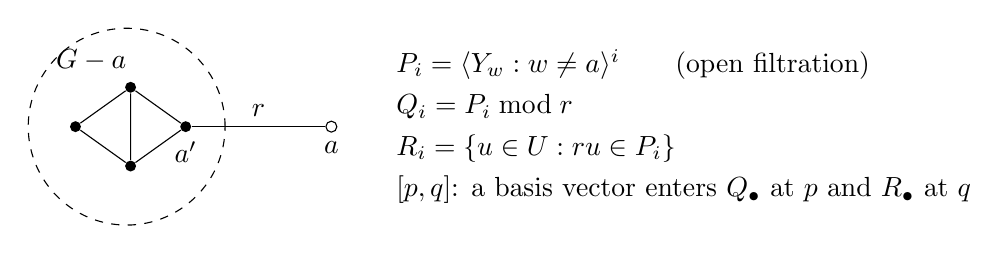
\begin{tikzpicture}[v/.style={circle,fill,inner sep=1.4pt},o/.style={circle,draw,fill=white,inner sep=1.4pt}]
  \draw[dashed] (0,0) circle (1.25);
  \node at (-0.45,0.85) {$G-a$};
  \node[v] (b) at (0.75,0) {};
  \node[v] (c1) at (0.05,0.5) {};
  \node[v] (c2) at (0.05,-0.5) {};
  \node[v] (c3) at (-0.65,0) {};
  \draw (b)--(c1)--(c3)--(c2)--(b) (c1)--(c2);
  \node[o] (a) at (2.6,0) {};
  \draw (b) -- node[above]{$r$} (a);
  \node[below=2pt] at (b) {$a'$};
  \node[below=2pt] at (a) {$a$};
  \node[align=left,anchor=west] at (3.3,0) {$P_i=\langle Y_w:w\ne a\rangle^i$\qquad (open filtration)\\[3pt]
     $Q_i=P_i\bmod r$\\[3pt]
     $R_i=\{u\in U:ru\in P_i\}$\\[3pt]
     $[p,q]$: a basis vector enters $Q_\bullet$ at $p$ and $R_\bullet$ at $q$};
\end{tikzpicture}
\caption{A marked leaf edge $r$ joining the leaf $a$, drawn open, to
$a'$. The open filtration $P_\bullet$ omits the generator at $a$. Writing
elements as $u+rv$ with $u,v$ in the algebra $U$ of the contracted graph,
$P_\bullet$ induces two filtrations $Q_\bullet$ and $R_\bullet$ of $U$.
A basis adapted to both assigns to each basis vector its boundary state
$[p,q]$ (Lemma~\ref{lem:split}).}
\label{fig:boundary-state}
\end{figure}

Splitting, assembly, and the gap bound hold for every normalized
nondegenerate $f$. For extension through bivalent vertices and the tail and neck
recurrences we assume $f=u+\alpha u^2+\beta u^3+\cdots$ with
$\alpha\ne0$. We use the generators $Y_v=f(X_v)$ of~\eqref{eq:gensY}.
For a finite set $S$ in a commutative algebra, $\langle S\rangle^i$
denotes the span of products of at most $i$ elements of $S$.
Every filtration is zero in negative degrees. Only $\alpha$ enters
the path-extension rule and only $\alpha,\beta$ enter the terminal
calculations; the attached boundary data may depend on higher coefficients.

\subsection{Boundary filtrations and their states}
\label{sec:split}

Let \(r\) be a leaf edge of a graph \(G\), joining a leaf vertex \(a\) to
\(a'\). Write \(r\) also for its edge variable \(\varphi_r\). Deleting
\(r\) isolates \(a\), so \(\CC^f_{G-r}\) is naturally identified with
\(\CC^f_{G/r}\). Under this identification the deletion map
\(j_r^*\) is evaluation at \(r=0\). We identify \(\CC^f_{G/r}\), as an
unfiltered algebra, with its image under the contraction embedding
\(\pi_r^*\).

Since \(Y_a=\pm r\), omitting the leaf generator gives the
\emph{open filtration}
\begin{equation}
\label{eq:open}
P_i=\bigl\langle Y_w:w\in V(G)\smallsetminus\{a\}\bigr\rangle^i
\subset\CC^f_G.
\end{equation}
This filtration is exhaustive. Indeed,
\(X_a=-\sum_{w\ne a}X_w\), and each \(X_w\) is a polynomial in
\(Y_w\), by Proposition~\ref{prop:same-algebra}. Thus the omitted generator
\(Y_a=f(X_a)\) belongs to the algebra generated by the other \(Y_w\).
The full, or \emph{closed}, filtration is \(P_i+rP_{i-1}\).

\begin{lemma}[Leaf splitting and boundary states]
\label{lem:split}
Put \(U=\CC^f_{G/r}\). Then:
\begin{enumerate}[(i)]
\item As vector subspaces of \(\Phi_G\),
\[
\CC^f_G=U\oplus rU,
\]
where \(U\) is the \(r\)-free part and multiplication by \(r\) is
injective on \(U\).
\item The image filtration \(Q_i=j_r^*(P_i)\) is
\(\CC^{f,i}_{G/r}\). Define a second filtration on \(U\) by
\[
R_i=\{u\in U:ru\in P_i\}.
\]
Then \(P_i\cap(r)=rR_i\).
\item There is a basis \(\{e_\lambda\}\) of \(U\), with nonnegative
integers \((p_\lambda,q_\lambda)\), such that
\[
Q_i=\Span\{e_\lambda:p_\lambda\le i\},\qquad
R_i=\Span\{e_\lambda:q_\lambda\le i\}.
\]
There are lifts
\(\widetilde e_\lambda=e_\lambda+ra_\lambda\in P_{p_\lambda}\),
with \(a_\lambda\in U\), for which
\begin{equation}
\label{eq:P-decomp}
P_i=\Span\{\widetilde e_\lambda:p_\lambda\le i\}
\oplus r\Span\{e_\lambda:q_\lambda\le i\}.
\end{equation}
\end{enumerate}
\end{lemma}

\begin{proof}
By Proposition~\ref{prop:same-algebra}, \(\CC^f_G=\CC_G\) as subalgebras of
\(\Phi_G\). The graded exact sequence~\eqref{eq:exact} identifies its
\(r\)-free part with \(U\). Since \(r\in\CC_G\) and
\(\delta_r(ru)=u\) for \(u\in U\), multiplication by \(r\) splits
that sequence. This proves (i). Evaluating the generators in~\eqref{eq:open}
at \(r=0\) gives precisely the vertex generators of \(G/r\), proving (ii).

For (iii), both \(Q_\bullet\) and \(R_\bullet\) are exhaustive
filtrations on the finite-dimensional space \(U\), with
\(Q_{-1}=R_{-1}=0\). For every \(p,q\ge0\)
choose a complement \(W_{p,q}\) such that
\[
Q_p\cap R_q=
\bigl((Q_{p-1}\cap R_q)+(Q_p\cap R_{q-1})\bigr)\oplus W_{p,q},
\]
and put \(w_{a,b}=\dim W_{a,b}\). We show by induction on \(p+q\) that
\begin{equation}\label{eq:two-flag-splitting}
Q_p\cap R_q=\bigoplus_{a\le p,\ b\le q}W_{a,b}.
\end{equation}
For \(p+q=0\) this is the definition of \(W_{0,0}\). In general, let
\(A=Q_{p-1}\cap R_q\) and \(B=Q_p\cap R_{q-1}\). By the inductive
hypothesis, \(A+B\) is spanned by the \(W_{a,b}\) with
\((a,b)\le(p,q)\) and \((a,b)\ne(p,q)\). Since
\(A\cap B=Q_{p-1}\cap R_{q-1}\), the inductive hypothesis also gives
\[
\dim(A+B)=\dim A+\dim B-\dim(A\cap B)
=\sum_{\substack{(a,b)\le(p,q)\\(a,b)\ne(p,q)}}w_{a,b}.
\]
Thus these spaces span \(A+B\) and their dimensions add up to
\(\dim(A+B)\), so their sum is direct. Adding \(W_{p,q}\)
proves~\eqref{eq:two-flag-splitting}. Since \(R_q=U\) for large \(q\), \eqref{eq:two-flag-splitting} gives
\(Q_p=\bigoplus_{a\le p}\bigoplus_bW_{a,b}\), and similarly for \(R_q\).
Let \(\{e_\lambda\}\) be the union of bases of the nonzero \(W_{p,q}\),
and give the basis vectors of \(W_{p,q}\) the state \((p,q)\). This basis
is adapted to both filtrations. Since \(Q_i=j_r^*(P_i)\), each
\(e_\lambda\) has a lift in \(P_{p_\lambda}\). The exact sequence
\[
0\longrightarrow rR_i\longrightarrow P_i
\xrightarrow{\ j_r^*\ }Q_i\longrightarrow0
\]
gives~\eqref{eq:P-decomp}, and (i) shows that its lifts have the asserted
form. In particular, \(r\widetilde e_\lambda=re_\lambda\).
\end{proof}

For an exhaustive increasing filtration $F_\bullet$, the \emph{birth degree} of a
nonzero vector $v$ is $\min\{i:v\in F_i\}$. We call
$[p_\lambda,q_\lambda]$ a \emph{boundary state}. The first
entry is the birth degree of \(e_\lambda\) in the \emph{image}
filtration \(Q_\bullet\); it need not be the birth degree of its
\(r\)-free representative in \(P_\bullet\). The second entry is the
birth degree of \(re_\lambda\) in \(P_\bullet\). The multiplicities
of the states are independent of the adapted bases and lifts, since
\begin{equation}
\label{eq:state-multiplicity}
\#\{\lambda:(p_\lambda,q_\lambda)=(p,q)\}
=\dim(Q_p\cap R_q)-\dim(Q_{p-1}\cap R_q)
-\dim(Q_p\cap R_{q-1})+\dim(Q_{p-1}\cap R_{q-1}).
\end{equation}
Reorientation preserves the boundary states as well. Its signed map
carries the open generators to the corresponding open generators and
commutes with evaluation at $r=0$. It sends $r$ to $\pm r$, so the
induced map on $U$ also carries each $R_i$ to its reoriented counterpart.
Thus it identifies both filtrations and all their intersections.

\begin{example}\label{ex:path-states}
For a single edge $r$ with one endpoint open, $U=\K$ and the retained
endpoint generator is $\pm r$, so the only state is $[0,1]$.
For the path of Example~\ref{ex:two-edge-path}, mark the edge $b$ with
leaf $3$. Then $U=\K[a]/(a^2)$ and the open filtration is generated
by $a$ and $b-a-2\alpha ab$. In either case $Q_0=\K$ and $Q_1=U$.

If $\alpha\ne0$, then $ab\notin P_1$,
$R_1=\K(1-2\alpha a)$ and $R_2=U$. The basis
$1,1-2\alpha a$ is simultaneously adapted, with states $[0,2]$ and
$[1,1]$. The closed Hilbert series is $1+3t$.
If $\alpha=0$, then $P_1=\Span\{1,a,b\}$,
$R_1=\K\,1$ and $R_2=U$. The basis $1,a$ instead gives states
$[0,1]$ and $[1,2]$, with closed series $1+2t+t^2$.
Thus the boundary data record both the change in the filtration and
how the two directions interact with the next attachment.
\end{example}


The lifts in~\eqref{eq:P-decomp} can be removed from all local
calculations. This is the principle behind every rule below.
The old graph spaces serve as coefficient spaces; the new multiplications
involve only the displayed boundary and vertex variables. The required
changes of basis are linear over these local variables, not algebra
automorphisms of the old graph algebras.

\begin{lemma}[Block decomposition]\label{lem:block}
Keep the notation of Lemma~\ref{lem:split}, and let $\Lambda$ be the
algebra of finitely many further edge variables, adjoined at the leaf
$a$. The $\Lambda[r]/(r^2)$-linear map
\[
\Psi\colon U\otimes\Lambda[r]/(r^2)\longrightarrow U\otimes\Lambda[r]/(r^2),
\qquad \Psi(e_\lambda)=e_\lambda+ra_\lambda,
\]
is invertible and commutes with multiplication by every element of
$\Lambda[r]/(r^2)$. It carries the direct sum, over $\lambda$, of the
blocks $e_\lambda\bigl(\K\,1\oplus\K\,r\bigr)$, in which $1$ enters
in degree $p_\lambda$ and $r$ in degree $q_\lambda$, onto the
filtration $P_\bullet$. Consequently, every filtration obtained from
$P_\bullet$ by adjoining generators that lie in $\Lambda[r]/(r^2)$ is
the direct sum of the corresponding filtrations of the blocks, and so
are its image and kernel-coefficient filtrations at any new boundary
variable in $\Lambda$.
\end{lemma}
\begin{proof}
The map has the form $I+rA$, with inverse $I-rA$, and it is linear over
$\Lambda[r]/(r^2)$ by definition. It maps $e_\lambda$ to
$\widetilde e_\lambda$ and $re_\lambda$ to $r\widetilde e_\lambda=re_\lambda$,
so~\eqref{eq:P-decomp} gives the assertion about $P_\bullet$. Adjoining
generators from $\Lambda[r]/(r^2)$ commutes with $\Psi$, and so do
reduction modulo a new boundary variable and multiplication by it.
Multiplicativity of $\Psi$ is not needed.
\end{proof}

To record a boundary calculation without choosing an adapted basis,
let $\mathcal S$ be the free abelian group on symbols $[p,q]$, with
$p,q\ge0$. Give it the $\Z[t]$-module structure
\[
 t[p,q]=[p+1,q+1].
\]
Thus multiplication by $t$ raises both birth degrees by one. If
$\mu_{p,q}(P)$ is the multiplicity in~\eqref{eq:state-multiplicity},
define the \emph{boundary-state sum} of the open filtration $P_\bullet$ by
\begin{equation}\label{eq:boundary-state-sum}
 \mathsf S(P_\bullet)=\sum_{p,q\ge0}\mu_{p,q}(P)[p,q]\in\mathcal S.
\end{equation}
This finite sum has nonnegative integer coefficients. Formal differences
in $\mathcal S$ will be used only to express linear identities between
such sums. When a state sum is written as $\sum_j a_j(t)[0,j]$, its
constant term means $\sum_j a_j(0)[0,j]$; the exponents of $t$ retain
the common birth-degree shifts.

\subsection{Assembly and bounded gaps}
\label{sec:boundary-assembly}

Let $e$ be a bridge of $G$. Cutting $G$ at $e$ gives two marked
graphs; each contains $e$ as its marked leaf edge, whose leaf is the
endpoint of $e$ on the other side. The generators of $G$ are the open
generators of the two sides. Hence the Hilbert series of $G$ is the sum,
over all pairs of states $[p,q]$ and $[p',q']$ of the two sides, of the
\emph{closing evaluation}
\begin{equation}\label{eq:edge-closing}
\mathsf E([p,q],[p',q'])
=t^{p+p'}+t^{\min(q+p',p+q')}.
\end{equation}
Indeed, by Lemma~\ref{lem:block} applied on both sides it suffices to
take one state on each side. Since $r^2=0$, the products of $1$ and $r$
from the two sides give $1$ in degree $p+p'$ and $r$ in degree
$\min(q+p',p+q')$. Reorienting the shared edge on one side, with the
signed identification just described, changes neither birth degree.


Fix a bound $D$ for the vertex degrees. Consider a vertex $v$ of degree
$r+1\le D$, with one incoming edge variable $x_j$ for each of the
pairwise disjoint incoming marked pieces $B_1,\ldots,B_r$ joined at $v$,
and an outgoing variable $z$
(Figure~\ref{fig:calculus}(b)). Its new generator is
\[
y=f(z-x_1-\cdots-x_r)
\quad\text{in}\quad
\Phi^{\rm loc}_r=\K[x_1,\ldots,x_r,z]/(x_1^2,\ldots,x_r^2,z^2).
\]
For incoming states $[p_j,q_j]$, put $d_j=q_j-p_j$.
After subtracting the common degree shift $\sum p_j$, the local
filtration is spanned by
\begin{equation}\label{eq:branch-local-columns}
x_Sy^k,\qquad S\subseteq\{1,\ldots,r\},\quad 0\le k\le r+1,
\qquad\text{at degree }\sum_{j\in S}d_j+k.
\end{equation}
Relative degrees may be negative; restoring the common shift gives the
actual filtration. Higher powers of $y$ vanish.
By Lemma~\ref{lem:block}, applied to each branch, each tuple of incoming
states can be treated independently, and the outgoing state
multiplicities are added.
If $P_i$ is the local span, $Q_i=P_i\bmod z$, and $zR_i=P_i\cap(z)$,
these multiplicities can be read from
\begin{equation}\label{eq:local-intersection-rank}
\dim(Q_i\cap R_j)
=\rank(zP_i)+\rank(P_j)-\rank(P_j+zP_i)
\end{equation}
by the two differences of~\eqref{eq:state-multiplicity}.
Here $\rank$ of a displayed span denotes its vector-space dimension.
Formula~\eqref{eq:local-intersection-rank} avoids choices of kernel bases.

\begin{lemma}[Bounds on boundary gaps]\label{lem:boundary-gap}
Let $G$ have maximum non-loop degree $D$, and let the non-leaf endpoint
of the marked leaf edge $r$ have non-loop degree $d$. For every
normalized nondegenerate $f$, the filtrations of Lemma~\ref{lem:split}
satisfy
\begin{equation}\label{eq:boundary-gap-inclusions}
Q_i\subseteq R_{i+D},\qquad R_i\subseteq Q_{i+d-2}.
\end{equation}
In particular, each boundary state satisfies
\begin{equation}\label{eq:boundary-gap-bound}
2-d\le q-p\le D.
\end{equation}
\end{lemma}
\begin{proof}
If $a$ is the marked leaf, then $X_a=\pm r$ and
$X_a=-\sum_{v\ne a}X_v$. Each $X_v=f^{-1}(Y_v)$ can be expressed by a
polynomial of degree at most $\deg v\le D$ in $Y_v$. Thus $r\in P_D$.
Multiplying a lift in $P_i$ of $u\in Q_i$ by $r$ gives
$ru\in P_{i+D}$, proving the first inclusion.
Only the generator at the other endpoint $b$ involves $r$.
Coefficient extraction therefore gives
\[
\delta_r(P_i)\subseteq f'(\overline X_b)Q_{i-1},
\qquad \overline X_b=j_r^*X_b.
\]
Since $\overline X_b^d=0$, the factor $f'(\overline X_b)$ is a polynomial
of degree at most $d-1$ in $f(\overline X_b)$. It follows that
$\delta_r(P_i)\subseteq Q_{i+d-2}$. Apply this to $ru\in P_i$ to obtain
the second inclusion. The state bounds follow by applying the two
inclusions to a simultaneous adapted basis.
\end{proof}


\Needspace{8\baselineskip}
\subsection{Extending a path by one edge}
\label{sec:boundary-propagation}

In this subsection $f=u+\alpha u^2+\cdots$ with $\alpha\ne0$.
Start with a graph whose marked leaf edge has variable $r$ and whose
open filtration is $P_\bullet$. Attach one new edge, with variable $s$,
at the marked leaf. The old leaf becomes a bivalent vertex; the new
leaf is the marked open endpoint. With compatible orientations, the
new vertex generator is
\[
 y=f(s-r)=s-r-2\alpha rs,
\]
and the new open filtration is
\[
 \widetilde P_i=\sum_{k\ge0}y^kP_{i-k}
              =P_i+yP_{i-1}+rsP_{i-2}.
\]
We call this operation \emph{path extension}. The following lemma
shows that $\mathsf S(\widetilde P_\bullet)$ depends only on
$\mathsf S(P_\bullet)$ and defines the \emph{path-extension operator}
$T:\mathcal S\to\mathcal S$. Iterating $T$ corresponds to successive
one-edge extensions; it is an operator on state sums, not a graph-algebra
homomorphism.

\begin{lemma}[One-edge extension]
\label{lem:boundary-transition}
The identity $\mathsf S(\widetilde P_\bullet)=T\mathsf S(P_\bullet)$
holds, where $T$ is the $\Z[t]$-linear operator
\begin{equation}
\label{eq:boundary-transition}
T[p,q]=
\begin{cases}
[p,p+1]+[q,q+1],&q\le p,\\
[p,p+2]+[p+1,p+1],&q=p+1,\\
[p,q]+[p+1,p+2],&q\ge p+2.
\end{cases}
\end{equation}
\end{lemma}

\begin{proof}
By the preceding change of basis it suffices to start with a single
state \([p,q]\) in \(\K[r]/(r^2)\). Since
\(y^2=-2rs\), \(ry=rs\), and \(y^3=ry^2=0\), the new filtration is
spanned by
\[
1\ \text{from degree }p,\quad r\ \text{from degree }q,\quad
 y\ \text{from degree }p+1,\quad
rs\ \text{from degree }\min(p+2,q+1).
\]
Set
\(a=\min(p+1,q)\), \(b=\min(p+2,q+1)\), and
\(c=\max(p+1,q)\). Its image and kernel-coefficient filtrations at
\(s\) are
\begin{equation}
\label{eq:transition-flags}
Q_i^{\rm new}=\Span\{1:p\le i,\ r:a\le i\},\qquad
R_i^{\rm new}=\Span\{r:b\le i,\ 1-2\alpha r:c\le i\}.
\end{equation}
Indeed, the image of \(y\) is \(-r\), and its cancellation with
\(r\) gives \(y+r=s(1-2\alpha r)\). These are all possibilities
for a kernel element. In the three cases of~\eqref{eq:boundary-transition},
simultaneous adapted bases for~\eqref{eq:transition-flags} are respectively
\[
(1-2\alpha r,r),\qquad (1,1-2\alpha r),\qquad (1,r).
\]
Their birth degrees give the table. The middle pair is a basis because
\(\alpha\ne0\).
\end{proof}

In Example~\ref{ex:path-states}, the passage from one edge to the open
path with two edges is the case $q=p+1$ of~\eqref{eq:boundary-transition}:
$T[0,1]=[0,2]+[1,1]$.

We next identify the polynomial governing $T$.
Put
\[
e_0=[0,0],\qquad e_1=[0,1],\qquad e_2=[0,2],\qquad
\mathcal V=\Z[t]e_0\oplus\Z[t]e_1\oplus\Z[t]e_2.
\]

\begin{lemma}[The path-extension operator and its stationary part]
\label{lem:propagation-polynomial}
The submodule \(\mathcal V\) is \(T\)-invariant. In the ordered basis
\(e_0,e_1,e_2\), the restriction of \(T\) has transfer matrix
\begin{equation}
\label{eq:propagation-matrix}
M=\begin{pmatrix}0&t&0\\2&0&t\\0&1&1\end{pmatrix},\qquad
\chi(z)=\det(zI-M)
=z^3-z^2-3tz+2t.
\end{equation}
For \(q\ge p+2\) the state difference
\begin{equation}
\label{eq:stationary-state}
z_{p,q}=[p,q]-[p,p+2]
\end{equation}
is stationary: \(Tz_{p,q}=z_{p,q}\). On all of \(\mathcal S\),
\begin{equation}
\label{eq:propagation-annihilator}
(T-I)\chi(T)T=0.
\end{equation}
\end{lemma}

\begin{proof}
The transition rule gives
\[
Te_0=2e_1,\qquad Te_1=te_0+e_2,\qquad Te_2=te_1+e_2,
\]
which proves~\eqref{eq:propagation-matrix}. Hence \(\chi(T)\) vanishes
on \(\mathcal V\) by the Cayley--Hamilton identity. Applying the
last row of~\eqref{eq:boundary-transition} to both terms
of~\eqref{eq:stationary-state} proves stationarity.
If \(q\le p\), then \(T[p,q]=(t^p+t^q)e_1\in\mathcal V\).
If \(q=p+1\), the state already lies in \(\mathcal V\).
If \(q\ge p+2\), it is the sum of \(t^pe_2\) and \(z_{p,q}\).
Thus \(T\mathcal S\) is contained in the sum of \(\mathcal V\)
and the stationary submodule, proving~\eqref{eq:propagation-annihilator}.
\end{proof}

\begin{proposition}[Intrinsic stationary boundary data]
\label{prop:boundary-enlargement}
For an open boundary filtration $P_\bullet$ on $A=U\oplus rU$, put
\begin{equation}\label{eq:boundary-enlargement}
\widehat P_i=P_i+rP_{i-2}.
\end{equation}
This is a multiplicative filtration. It replaces a state $[p,q]$ by
$[p,\min(q,p+2)]$, and
\begin{equation}\label{eq:boundary-enlargement-quotient}
\widehat P_i/P_i\simeq Q_{i-2}/(Q_{i-2}\cap R_i).
\end{equation}
After adjoining a bivalent vertex, inclusion of the old edge algebra
induces isomorphisms
$\widehat P_i/P_i\simeq\widehat{\widetilde P}_i/\widetilde P_i$
for every $i$, compatible with the maps between consecutive levels.
\end{proposition}
\begin{proof}
Multiplicativity follows from $r^2=0$ and that of $P_\bullet$.
Also $rP_j=rQ_j$ and $P_i\cap rU=rR_i$, giving
\eqref{eq:boundary-enlargement-quotient} and the state description.

Write $y=s-r-2\alpha rs$. Since $y^2=-2rs$ and $y^3=0$,
\[
\widetilde P_i=P_i+yP_{i-1}+rsP_{i-2}.
\]
If $a_0+ya_1+rsa_2$ has no $s$-term, then
$(1-2\alpha r)a_1+ra_2=0$. Multiplying by $r$ gives $ra_1=0$,
so the element equals $a_0\in P_i$. Hence
$\widetilde P_i\cap A=P_i$.
Furthermore $sy=-rs$ implies
\[
\widehat{\widetilde P}_i=\widetilde P_i+sP_{i-2}.
\]
For $a\in P_{i-2}$, the identity
$sa-ra=ya+2\alpha rsa\in\widetilde P_i$ changes the last summand to
$rP_{i-2}$. Inclusion therefore identifies the two quotients, using
$\widetilde P_i\cap A=P_i$. All maps are induced by the same inclusions
of edge algebras, so they commute with passage to the next level.
\end{proof}

These quotients measure the change from $P_\bullet$ to the enlarged
filtration $\widehat P_i=P_i+rP_{i-2}$, in which multiplication by $r$
has filtration degree at most two. They give a basis-independent
interpretation of the stationary state differences.

\subsection{The calculus in summary}
\label{sec:calculus}

\begin{theorem}[Boundary-state calculus]\label{thm:calculus}
Let $f$ be normalized and nondegenerate, and let $D$ bound the vertex
degrees, with $D\ge1$.
\begin{enumerate}[(i)]
\item \emph{Closing.} If a bridge $e$ cuts $G$ into two marked graphs
with boundary states $s_\lambda$ and $s'_\mu$ at $e$, then
$\hs^f_G=\sum_{\lambda,\mu}\mathsf E(s_\lambda,s'_\mu)$, with
$\mathsf E$ as in~\eqref{eq:edge-closing}.
\item \emph{Branching.} Let $B_1,\ldots,B_r$ be incoming marked pieces,
pairwise disjoint before attachment, with marked edge variables
$x_1,\ldots,x_r$. Identify their open leaf endpoints at a new vertex $v$, and attach one further edge $z$ with an open leaf
endpoint. The states at $z$ are obtained by summing, over all tuples of states
$[p_j,q_j]$ of the branches, the outgoing states of the local
filtration~\eqref{eq:branch-local-columns}, multiplied by
$t^{\sum_jp_j}$. The local computation takes place in an algebra of
dimension $2^{r+1}$ and depends only on the gaps $q_j-p_j$ and on $f$
modulo $u^{r+2}$.
\item \emph{Path extension.} If $\alpha\ne0$ and $r=1$, the rule in (ii)
is the operator $T$ of~\eqref{eq:boundary-transition}.
\item \emph{Gaps.} Every state satisfies $2-D\le q-p\le D$.
\end{enumerate}
In particular, the Hilbert series of a tree is computed by rooting it at
an edge, starting with the state $[0,1]$ at each leaf, applying (ii) at
each vertex, and closing by (i).
\end{theorem}
\begin{proof}
Part (i) is~\eqref{eq:edge-closing}. Part (ii) is the discussion
following~\eqref{eq:branch-local-columns}, which uses
Lemma~\ref{lem:block} for each branch and the rank
formula~\eqref{eq:local-intersection-rank}; only $f$ modulo $u^{r+2}$
enters, because $(z-\sum_jx_j)^{r+2}=0$. Part (iii) is
Lemma~\ref{lem:boundary-transition}, and (iv) is
Lemma~\ref{lem:boundary-gap}. A leaf, regarded as a branch, is a single
edge with one open endpoint and has the state $[0,1]$
(Example~\ref{ex:path-states}).
\end{proof}

\begin{figure}[htbp]
\centering
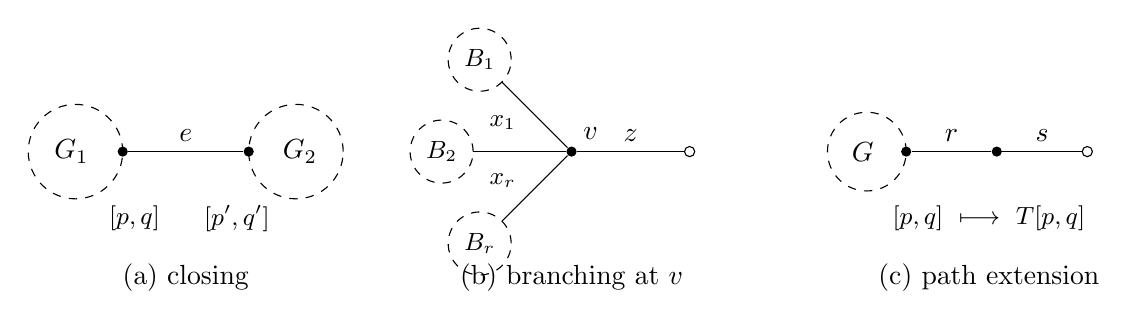
\begin{tikzpicture}[v/.style={circle,fill,inner sep=1.3pt},o/.style={circle,draw,fill=white,inner sep=1.3pt}]
\begin{scope}
 \draw[dashed] (0,0) circle (0.6); \node at (-0.05,0) {$G_1$};
 \draw[dashed] (2.8,0) circle (0.6); \node at (2.85,0) {$G_2$};
 \node[v] (u) at (0.6,0) {}; \node[v] (w) at (2.2,0) {};
 \draw (u) -- node[above]{$e$} (w);
 \node at (0.75,-0.85) {\small$[p,q]$};
 \node at (2.05,-0.85) {\small$[p',q']$};
 \node at (1.4,-1.6) {(a) closing};
\end{scope}
\begin{scope}[xshift=6.3cm]
 \node[v] (c) at (0,0) {};
 \node[above right=1pt] at (c) {$v$};
 \node[o] (z) at (1.5,0) {};
 \draw (c) -- node[above]{$z$} (z);
 \foreach \ang/\j in {135/1,180/2,225/r}{
   \draw[dashed] (\ang:1.65) circle (0.4);
   \node at (\ang:1.65) {\small$B_{\j}$};
   \draw (c) -- (\ang:1.25);}
 \node at (157:0.95) {\small$x_1$};
 \node at (203:0.95) {\small$x_r$};
 \node at (0,-1.6) {(b) branching at $v$};
\end{scope}
\begin{scope}[xshift=10.6cm]
 \draw[dashed] (-0.55,0) circle (0.5); \node at (-0.6,0) {$G$};
 \node[v] (a) at (-0.05,0) {}; \node[v] (b) at (1.1,0) {}; \node[o] (c) at (2.25,0) {};
 \draw (a) -- node[above]{$r$} (b) -- node[above]{$s$} (c);
 \node at (1.0,-0.85) {\small$[p,q]\ \longmapsto\ T[p,q]$};
 \node at (1.0,-1.6) {(c) path extension};
\end{scope}
\end{tikzpicture}
\caption{The rules of Theorem~\ref{thm:calculus}. (a) The states of the
two sides of a bridge $e$ close to the Hilbert series of the whole graph.
(b) At a vertex $v$, the states of the branches along $x_1,\ldots,x_r$
determine the states at the open edge $z$. (c) Inserting a bivalent
vertex acts on states by the path-extension operator $T$. Open circles are
open leaves.}
\label{fig:calculus}
\end{figure}

\subsection{Tail families}
\label{sec:tails}

Given  a graph $G=(V,E)$ with a marked vertex $v\in V$,
we consider three families of graphs with tails: the \emph{straight-tail}  $G_n$, the \emph{forked-tail} $\widetilde{G}_n$, and the \emph{double-edged} $G^b_n$ extensions of $G$ (Figure~\ref{fig:tails}).

\begin{figure}[htbp]
\centering
$G_n=$\,\begin{minipage}[c]{7.1cm}
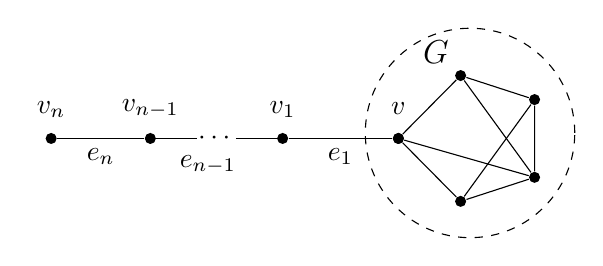
\begin{tikzpicture}[scale=0.7,vertex/.style={circle, fill=black, inner sep=0pt, minimum size=4pt} ]
  \node[vertex] (vn)  at (0.0, 0) {};
  \node[vertex] (vn1) at (1.8, 0) {};
  \node[vertex] (v1)  at (4.2, 0) {};
  \node[vertex] (v0)  at (6.3, 0) {};
  \node[vertex] (u0)  at (6.3, 0) {};
  \node[above=4pt] at (vn)  {$v_n$};
  \node[above=4pt] at (vn1) {$v_{n-1}$};
  \node[above=4pt] at (v1)  {$v_1$};
  \node[above=5pt] at (v0)  {$v$};
  \draw (vn)  -- node[below]{$e_n$} (vn1);
  \draw (vn1) -- node[below]{\phantom{YYY}$e_{n-1}$} (2.65, 0);
  \draw (3.35, 0) -- (v1);
  \draw (v1)  -- node[below]{$e_1$}(v0);
  \node at (3.0, 0) {$\cdots$};
  \pgfmathsetmacro{\R}{1.2}
 \pgfmathsetmacro{\cx}{7.8}
  \node[vertex] (u1) at ({\cx + \R*cos(108)}, {\R*sin(108)})  {};
  \node[vertex] (u2) at ({\cx + \R*cos(36)},  {\R*sin(36)})   {};
  \node[vertex] (u3) at ({\cx + \R*cos(-36)}, {\R*sin(-36)})  {};
  \node[vertex] (u4) at ({\cx + \R*cos(-108)},{\R*sin(-108)}) {};
  \draw (u0) -- (u1) -- (u2) -- (u3) -- (u4) -- (u0);
  \draw (u1)--(u3);
  \draw (u2)--(u4);
  \draw (u0)--(u3);

  \draw[dashed] (\cx-.2, 0.1) circle (1.9);
\node[above left=1pt] at (u1)  {\large $G$};
\end{tikzpicture}
\end{minipage}\qquad
$\widetilde{G}_n=$\,\begin{minipage}[c]{7.2cm}
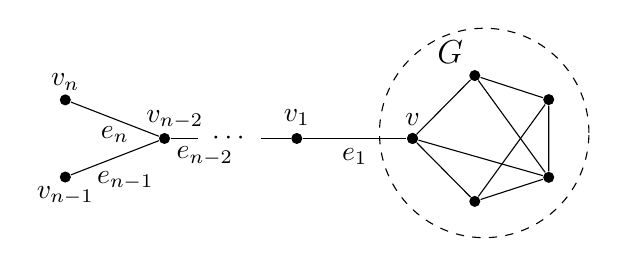
\begin{tikzpicture}[scale=0.7,vertex/.style={circle, fill=black, inner sep=0pt, minimum size=4pt} ]
  \node[vertex] (vn)  at (0.0, 0.7) {};
  \node[vertex] (vn1)  at (0.0, -0.7) {};
  \node[vertex] (vn2) at (1.8, 0) {};
  \node[vertex] (v1)  at (4.2, 0) {};
  \node[vertex] (v0)  at (6.3, 0) {};
  \node[vertex] (u0)  at (6.3, 0) {};
  \node[above=0pt] at (vn)  {$v_n$};
  \node[below=0pt] at (vn1) {$v_{n-1}$};
  \node[above=0pt] at (vn2)  {\phantom{Y}$v_{n-2}$};
  \node[above=1pt] at (v1)  {$v_1$};
  \node[above=1pt] at (v0)  {$v$};
  \draw (vn)  -- node[below=-1pt]{$e_n$} (vn2);
  \draw (vn1)  -- node[below=-1pt]{\phantom{Y}$e_{n-1}$} (vn2);
  \draw (vn2) -- node[below=-3pt]{\phantom{YY}$e_{n-2}$} (2.4, 0);
  \draw (3.55, 0) -- (v1);
  \draw (v1)  -- node[below]{$e_1$}(v0);
  \node at (3.0, 0) {$\cdots$};
  \pgfmathsetmacro{\R}{1.2}
  \pgfmathsetmacro{\cx}{7.8}
  \node[vertex] (u1) at ({\cx + \R*cos(108)}, {\R*sin(108)})  {};
  \node[vertex] (u2) at ({\cx + \R*cos(36)},  {\R*sin(36)})   {};
  \node[vertex] (u3) at ({\cx + \R*cos(-36)}, {\R*sin(-36)})  {};
  \node[vertex] (u4) at ({\cx + \R*cos(-108)},{\R*sin(-108)}) {};
  \draw (u0) -- (u1) -- (u2) -- (u3) -- (u4) -- (u0);
  \draw (u1)--(u3);
  \draw (u2)--(u4);
  \draw (u0)--(u3);
  \draw[dashed] (\cx-.2, 0.1) circle (1.9);
  \node[above left=1pt] at (u1)  {\large $G$};
\end{tikzpicture}
\end{minipage}\\[12pt]
$G^b_n=$\,\begin{minipage}[c]{7.1cm}
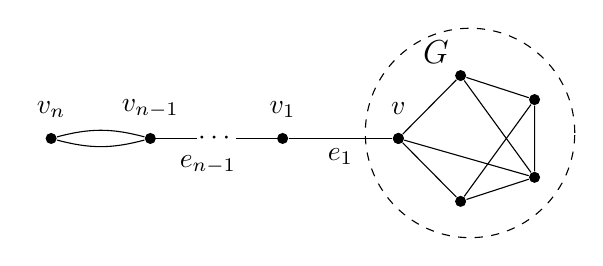
\begin{tikzpicture}[scale=0.7,vertex/.style={circle, fill=black, inner sep=0pt, minimum size=4pt} ]
  \node[vertex] (vn)  at (0.0, 0) {};
  \node[vertex] (vn1) at (1.8, 0) {};
  \node[vertex] (v1)  at (4.2, 0) {};
  \node[vertex] (v0)  at (6.3, 0) {};
  \node[vertex] (u0)  at (6.3, 0) {};
  \node[above=4pt] at (vn)  {$v_n$};
  \node[above=4pt] at (vn1) {$v_{n-1}$};
  \node[above=4pt] at (v1)  {$v_1$};
  \node[above=5pt] at (v0)  {$v$};
  \draw (vn) to[out=15,in=165, min distance=.5cm] (vn1);
  \draw (vn) to[out=-15,in=-165, min distance=.5cm] (vn1);
  \draw (vn1) -- node[below]{\phantom{YYY}$e_{n-1}$} (2.65, 0);
  \draw (3.35, 0) -- (v1);
  \draw (v1)  -- node[below]{$e_1$}(v0);
  \node at (3.0, 0) {$\cdots$};
  \pgfmathsetmacro{\R}{1.2}
  \pgfmathsetmacro{\cx}{7.8}
  \node[vertex] (u1) at ({\cx + \R*cos(108)}, {\R*sin(108)})  {};
  \node[vertex] (u2) at ({\cx + \R*cos(36)},  {\R*sin(36)})   {};
  \node[vertex] (u3) at ({\cx + \R*cos(-36)}, {\R*sin(-36)})  {};
  \node[vertex] (u4) at ({\cx + \R*cos(-108)},{\R*sin(-108)}) {};
  \draw (u0) -- (u1) -- (u2) -- (u3) -- (u4) -- (u0);
  \draw (u1)--(u3);
  \draw (u2)--(u4);
  \draw (u0)--(u3);
  \draw[dashed] (\cx-.2, 0.1) circle (1.9);
  \node[above left=1pt] at (u1)  {\large $G$};
\end{tikzpicture}
\end{minipage}
\caption{The straight-tail extension $G_n$, the forked-tail extension
$\widetilde G_n$ and the double-edged extension $G^b_n$ of a graph $G$
with a marked vertex $v$.}
\label{fig:tails}
\end{figure}

The straight-tail extension $G_n$, for $n\ge0$, attaches at $v$ a path
of length $n$, with vertices $v_0=v,v_1,\ldots,v_n$. The forked-tail
extension $\widetilde G_n$, for $n\ge2$, attaches two new leaf edges at
the terminal vertex $v_{n-2}$ of $G_{n-2}$; here $v_0=v$ when $n=2$.
The double-edged extension $G_n^b$, for $n\ge2$, is $G_n$ with one
additional edge joining $v_{n-1}$ to $v_n$.

The three families satisfy the same third-order recurrence. For the
forked and double-edged families, it follows from identities with the
straight-tail series. We use the operator
\begin{equation}\label{eq:L}
 L(a_n)=a_n-a_{n-1}-3t\,a_{n-2}+2t\,a_{n-3},
\end{equation}
whenever the four terms are defined.

\begin{theorem}
  \label{th:4t-rec}
  Let \(G\) be a graph with a marked vertex \(v\). Let   \(G_n, \widetilde{G}_n\),  and  \(G^b_n \) be
the  straight, forked and double-edged extensions defined above.
  Let \(H_n(t), \ \widetilde{H}_n(t),\)  and   \(H^b_n(t)\)  be the Hilbert series of the corresponding algebras \(\CC^f_{G_n}, \ \CC^f_{\widetilde{G}_n}\),  and  \(\CC^f_{G^b_n}\),
  where
  \begin{equation}
    \label{eq:func}
 f=u+\alpha u^2+\beta u^3+\ldots, \qquad \alpha\ne 0.
\end{equation}

Then:
  \begin{enumerate}
  \item[\textup{(i)}]
    The straight-tail Hilbert series satisfy the third-order recurrence
    $L(H_n)=0$, that is,
    \begin{equation}
      \label{eq:4t-rec}
    H_n=H_{n-1}+3tH_{n-2}-2tH_{n-3}, \qquad n\ge 4.
  \end{equation}

  \item[\textup{(ii)}]
    The forked tail family has the same Hilbert series as the straight tail:
    \[
      \widetilde H_n=H_n,  \qquad n\ge3.
    \]

  \item[\textup{(iii)}]
    For the double-edged family one has
    \[
      H_n^b=H_{n+1}-tH_{n-1}, \qquad   n\ge2.
    \]
    Consequently the double-edged Hilbert series satisfy the same recurrence
    \(L(H^b_n)=0\), that is,
    \[
      H_n^b=H_{n-1}^b+3tH_{n-2}^b-2tH_{n-3}^b,
      \qquad  n\ge 5.
    \]
  \end{enumerate}
\end{theorem}


For a boundary state define two \(\Z[t]\)-linear evaluations
\begin{equation}
\label{eq:boundary-evaluations}
\mathsf c[p,q]=t^p+t^{\min(q,p+1)},\qquad
\mathsf n[p,q]=t^p+t^{\min(q,p+2)}.
\end{equation}
They give its contributions to the Hilbert series of the closed filtration
\(P_i+rP_{i-1}\) and the augmented filtration \(P_i+rP_{i-2}\),
respectively. To see this, use~\eqref{eq:P-decomp}: the lift of the
quotient class still enters in degree \(p\), whereas its \(r\)-multiple
enters either in degree \(q\) or by multiplying that lift, with the
indicated shift.

\begin{lemma}
\label{lem:tail-evaluations}
For every state \(s\in\mathcal S\),
\begin{equation}
\label{eq:tail-evaluation-identities}
\mathsf n(Ts)=\mathsf n(s)+t\mathsf c(s),\qquad
\mathsf c(T^2s)=\mathsf n(s)+3t\mathsf c(s).
\end{equation}
\end{lemma}

\begin{proof}
Substitute the three cases of~\eqref{eq:boundary-transition}
into~\eqref{eq:boundary-evaluations}. For \(s=[p,q]\), the resulting
values are
\[
\begin{array}{c|c|c}
 &\mathsf n(Ts)&\mathsf c(T^2s)\\ \hline
q\le p &(t^p+t^q)(1+t)&(t^p+t^q)(1+3t)\\
q=p+1 &t^p(1+2t+t^2)&t^p(1+4t+3t^2)\\
q\ge p+2 &t^p(1+t+2t^2)&t^p(1+3t+4t^2).
\end{array}
\]
These agree with the two right-hand sides
of~\eqref{eq:tail-evaluation-identities}.
\end{proof}

The three terminal configurations can also be handled uniformly.

\begin{lemma}[Terminal evaluation]
\label{lem:terminal-evaluation}
Let \(E=B\otimes\K[r]/(r^2)\), where \(B\) is a finite-dimensional
commutative unital algebra and \(\dim B=d\). Suppose terminal generators
define a filtration \(M_\ell\) on \(E\) with
\begin{equation}
\label{eq:terminal-complement}
M_0=\K,\qquad M_1\xrightarrow{\ r=0\ }E/(r)
\text{ an isomorphism},\qquad M_2=E.
\end{equation}
Then an incoming state \([p,q]\) gives the filtration
\(F_i=M_{i-p}+rM_{i-q}\), whose Hilbert series is
\begin{equation}
\label{eq:terminal-evaluation}
H_{F_\bullet}(t)=(d-1)t\,\mathsf c[p,q]+\mathsf n[p,q].
\end{equation}
\end{lemma}

\begin{proof}
The hypotheses give \(M_1\cap rE=0\) and \(rM_1=rE\). If
\(q\le p\), the kernel \(rE\) is filled in degrees \(q,q+1\),
with dimensions \(1,d-1\), while the quotient is filled in degrees
\(p,p+1\), with the same dimensions. If \(q=p+1\), the vector
\(r\) adds one dimension to \(M_1\) in degree \(p+1\). If
\(q\ge p+2\), the extra summand arrives only when \(M_2=E\).
Thus the three Hilbert series are
\[
\begin{cases}
(t^p+t^q)(1+(d-1)t),&q\le p,\\
t^p(1+dt+(d-1)t^2),&q=p+1,\\
t^p(1+(d-1)t+dt^2),&q\ge p+2.
\end{cases}
\]
Each equals~\eqref{eq:terminal-evaluation}.
\end{proof}

\begin{lemma}[The three ends]
\label{lem:three-ends}
For an incoming state \(s\), the straight two-edge end and the forked
end both contribute \(3t\mathsf c(s)+\mathsf n(s)\). The doubled
one-edge end contributes \(2t\mathsf c(s)+\mathsf n(s)\).
\end{lemma}

\begin{proof}
For the straight and forked ends use
\(E=\K[r,s,u]/(r^2,s^2,u^2)\), so \(d=4\).
For the straight end the generators can be taken to be
\[
g_1=f(s-r),\qquad g_2=f(u-s),\qquad g_3=u.
\]
Modulo \(r\), their span together with \(1\) has basis
\(1,s,u,su\), since \(\alpha\ne0\). Moreover,
\[
g_1^2=-2rs,\quad g_2^2=-2su,\quad
g_1g_2=su-ru+rs,\quad g_1g_3=su-ru-2\alpha rsu.
\]
Hence quadratic products span \(rs,ru,su,rsu\). Together with
\(1,g_1,g_2,g_3\) they span \(E\), proving~\eqref{eq:terminal-complement}.

For the forked end the generators are \(h=f(s+u-r),s,u\). Their
images modulo \(r\), together with \(1\), again form a basis of
\(E/(r)\). The identities
\[
(h-s-u)^2=-4\alpha rsu,\qquad
hs=su-rs-2\alpha rsu,\qquad
hu=su-ru-2\alpha rsu
\]
show that quadratic products span all four monomials of degree at least
two. Thus~\eqref{eq:terminal-complement} holds here as well.

For the doubled end let \(s,s'\) be its two parallel edge variables and
put \(\sigma=s+s'\). Then \(\sigma^2=2ss'\) and \(\sigma^3=0\).
The terminal generators lie in
\(E=\K[r,\sigma]/(r^2,\sigma^3)\), with \(d=3\), and are
\[
h_1=f(\sigma-r),\qquad h_2=f(-\sigma).
\]
Their images modulo \(r\) are \(\sigma+\alpha\sigma^2\) and
\(-\sigma+\alpha\sigma^2\), which together with \(1\) form a
basis. Finally,
\[
h_2^2=\sigma^2,\qquad
h_1h_2=-\sigma^2+r\sigma+\alpha r\sigma^2,\qquad
(h_1+h_2)^2=-4\alpha r\sigma^2.
\]
Thus \(M_2=E\). Lemma~\ref{lem:terminal-evaluation}, with
\(d=4,4,3\), gives the assertions. Terms of \(f\) of degree at least four do not
enter these algebras, and none of these calculations restricts \(\beta\).
\end{proof}

\begin{proof}[Proof of Theorem~\ref{th:4t-rec}]
Orient the tail away from \(G\). For \(m\ge1\), let
\(P^{(m)}_i\) be the open filtration of \(\CC^f_{G_m}\) at its terminal
edge, whose variable is \(\varphi_m\), and let \(S_m\in\mathcal S\)
be its collection of boundary states. Denote by \(N_m(t)\) the
Hilbert series of the augmented filtration
\(P^{(m)}_i+\varphi_m P^{(m)}_{i-2}\), \(i\ge0\).
By Lemma~\ref{lem:boundary-transition} and~\eqref{eq:boundary-evaluations},
\[
S_{m+1}=TS_m,\qquad H_m=\mathsf c(S_m),\qquad
N_m=\mathsf n(S_m).
\]
Lemma~\ref{lem:tail-evaluations} gives
\begin{equation}
\label{eq:tail-two-identities}
N_m=N_{m-1}+tH_{m-1}\quad(m\ge2),\qquad
H_n=3tH_{n-2}+N_{n-2}\quad(n\ge3).
\end{equation}
Subtracting consecutive instances of the second equality and then
using the first gives, for \(n\ge4\),
\[
\begin{aligned}
H_n-H_{n-1}
&=3t(H_{n-2}-H_{n-3})+N_{n-2}-N_{n-3}\\
&=3tH_{n-2}-2tH_{n-3}.
\end{aligned}
\]
This proves (i).

For (ii), the straight and forked ends are attached to the open tail
\(G_{n-2}\), which has a terminal leaf when \(n\ge3\).
Lemma~\ref{lem:three-ends} gives
\[
\widetilde H_n=3tH_{n-2}+N_{n-2}=H_n.
\]
For (iii), attach the doubled end to the open tail \(G_{n-1}\).
The same lemma gives the uniform formula
\begin{equation}
\label{eq:double-end-uniform}
H_n^b=2tH_{n-1}+N_{n-1}\qquad(n\ge2).
\end{equation}
Comparing with~\eqref{eq:tail-two-identities} at \(n+1\) yields
\[
H_n^b=H_{n+1}-tH_{n-1}\qquad(n\ge2).
\]
In particular, the initial doubled tail requires no separate argument.
For \(n\ge5\), the four terms \(H^b_n,\ldots,H^b_{n-3}\) of
\(L(H_n^b)\) have indices at least \(2\), so each can be replaced by
this formula. Since \(L\) is \(\Z[t]\)-linear and commutes with index
shifts, (i) gives
\[
L(H_n^b)=L(H_{n+1})-tL(H_{n-1})=0,
\]
because \(n+1\ge4\) and \(n-1\ge4\).
This proves the last assertion.
\end{proof}

\begin{remark}
\label{rem:tail-initial}
The starting indices in (i) and (ii) cannot be lowered in general.
For \(G=K_3\) and \(f=u+\alpha u^2\), with \(\alpha\ne0\),
one computes \(L(H_3)=-t^3+t^4\). For \(G=K_{1,3}\) marked at
its center and the same \(f\), one has
\(\widetilde H_2-H_2=-t^2+t^3\). Both examples concern the initial
attachment to the marked vertex, before the uniform path-extension rule at
bivalent vertices applies.
\end{remark}

For paths the recurrence and four initial values give a closed form.

\begin{corollary}[Paths]\label{cor:path-series}
Let $f=u+\alpha u^2+\cdots$, with $\alpha\ne0$, and let $H_n$ be the Hilbert series of the path with
$n$ edges. Then
\begin{equation}\label{eq:path-series}
\sum_{n\ge0}H_n\,x^n=\frac{1+tx-tx^2}{1-x-3tx^2+2tx^3}.
\end{equation}
One has $H_0=1$ and $\deg H_n=\lceil n/2\rceil$ for all $n\ge0$.
For positive indices, the leading coefficient is $3^{r-1}$ when
$n=2r-1$, $r\ge1$, and $(m+8)3^{m-2}$ when $n=2m$, $m\ge1$.
(See~Table~\ref{tab:paths} for the first several values.)
\end{corollary}
\begin{proof}
Take $G$ to be a single vertex in Theorem~\ref{th:4t-rec}(i), so that
$L(H_n)=0$ for $n\ge4$. The initial values are $H_0=1$, $H_1=1+t$,
$H_2=1+3t$ (Example~\ref{ex:two-edge-path}) and $H_3=1+4t+3t^2$. For
the last, the open path with three edges has the states
$T^2[0,1]=[0,2]+3[1,2]$ by Lemma~\ref{lem:boundary-transition},
and closing with the leaf state $[0,1]$ gives
$(1+t)+3(t+t^2)$. These values also satisfy $L(H_3)=0$.
Multiplying the series by $1-x-3tx^2+2tx^3$ therefore leaves
$H_0+(H_1-H_0)x+(H_2-H_1-3tH_0)x^2=1+tx-tx^2$.

For the degrees, use $H_n=H_{n-1}+3tH_{n-2}-2tH_{n-3}$ and induction.
If $n=2r-1\ge5$, only the middle term reaches degree $r$, so the leading
coefficient is three times that of $H_{n-2}$. If $n=2m\ge4$, all three
terms reach degree $m$, and the leading coefficients satisfy
$c_{2m}=3^{m-1}+3c_{2m-2}-2\cdot3^{m-2}=3c_{2m-2}+3^{m-2}$, with
$c_2=3$. This gives $c_{2m}=(m+8)\,3^{m-2}$.
\end{proof}

\begin{table}[htbp]
\centering\renewcommand{\arraystretch}{1.12}
\begin{tabular}{rll}\toprule
$n$ & $H_n$ for $\alpha\ne0$ & $H_n$ for $f=u$\\\midrule
1 & $1+t$ & $1+t$\\
2 & $1+3t$ & $1+2t+t^2$\\
3 & $1+4t+3t^2$ & $(1+t)^3$\\
4 & $1+5t+10t^2$ & $(1+t)^4$\\
5 & $1+6t+16t^2+9t^3$ & $(1+t)^5$\\
6 & $1+7t+23t^2+33t^3$ & $(1+t)^6$\\
7 & $1+8t+31t^2+61t^3+27t^4$ & $(1+t)^7$\\
8 & $1+9t+40t^2+98t^3+108t^4$ & $(1+t)^8$\\\bottomrule
\end{tabular}
\caption{Hilbert series of paths with $n$ edges for normalized
nondegenerate parameters. The two columns correspond to $\alpha\ne0$
and $\alpha=0$, respectively.}
\label{tab:paths}
\end{table}

\begin{remark}[The value at $t=1$]\label{rem:t-equals-one}
At $t=1$ the characteristic polynomial factors as
$\chi(z)=(z-2)(z^2+z-1)$, and the numerator in~\eqref{eq:path-series}
cancels the second factor, leaving $\sum_n2^nx^n$: the path with $n$
edges has $2^n$ spanning forests. More generally, $H_n(1)=\dim\CC_{G_n}$
is $2^n$ times the number of spanning forests of $G$, in accordance with
the root $z=2$. For odd $n$, the top filtered piece of the path is
described explicitly in Lemma~\ref{lem:dual-path}; its dimension
$3^{r-1}$ is the leading coefficient above.
\end{remark}

\subsection{Neck families}
\label{sec:necks}


  Let   \(G'\) and \(G''\) be disjoint graphs
  with marked vertices $v'\in V(G')$ and $v''\in V(G'')$. Denote by \(G'*_nG''\) the graph obtained by joining
  \(G'\) and \(G''\) at \(v'\) and \(v''\) by a path of length $n$
(Figure~\ref{fig:neck}).

\begin{figure}[htbp]
\centering
$G'*_nG''=$\,\begin{minipage}[c]{9.1cm}
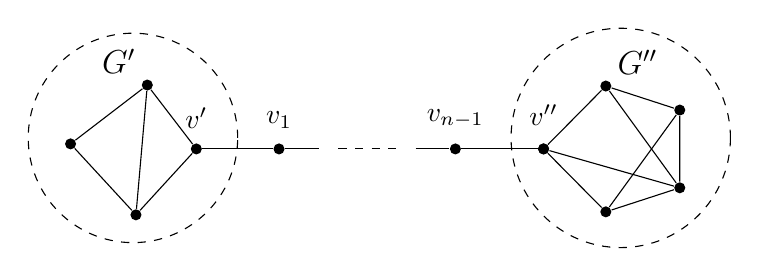
\begin{tikzpicture}[scale=0.7,vertex/.style={circle, fill=black, inner sep=0pt, minimum size=4pt} ]
  \node[vertex] (v0)  at (0.0, 0) {};
  \node[vertex] (v1) at (1.5, 0) {};
  \node[vertex] (vn1)  at (4.7, 0) {};
  \node[vertex] (vn)  at (6.3, 0) {};
  \node[vertex] (u0)  at (6.3, 0) {};
  \node (dl)  at (2.4, 0) {};
  \node (dr)  at (3.8, 0) {};
  \node[above=4pt] at (v0)  {$v'$};
  \node[above=4pt] at (v1) {$v_1$};
  \node[above=4pt] at (vn1)  {$v_{n-1}$};
  \node[above=5pt] at (vn)  {$v''$};
  \draw (vn)  --  (vn1);
  \draw (v1) --  (dl);
  \draw (dr) -- (vn1);
  \draw (v1)  -- (v0);
    \draw[dashed] (dl) -- (dr);
  \pgfmathsetmacro{\R}{1.2}
  \pgfmathsetmacro{\cx}{7.8}
  \pgfmathsetmacro{\cy}{-1.2}
  \node[vertex] (u1) at ({\cx + \R*cos(108)}, {\R*sin(108)})  {};
  \node[vertex] (u2) at ({\cx + \R*cos(36)},  {\R*sin(36)})   {};
  \node[vertex] (u3) at ({\cx + \R*cos(-36)}, {\R*sin(-36)})  {};
  \node[vertex] (u4) at ({\cx + \R*cos(-108)},{\R*sin(-108)}) {};
  \node[vertex] (w1) at ({\cy + \R*cos(75)}, {\R*sin(75)})  {};
  \node[vertex] (w2) at ({\cy + \R*cos(-85)},  {\R*sin(-85)})   {};
  \node[vertex] (w3) at ({\cy+.1 + \R*cos(-170)}, {.3+\R*sin(-170)})  {};
  \draw (v0) -- (w1) -- (w3) -- (w2) -- (v0);
  \draw (w1) -- (w2);
  \draw (u0) -- (u1) -- (u2) -- (u3) -- (u4) -- (u0);
  \draw (u1)--(u3);
  \draw (u2)--(u4);
  \draw (u0)--(u3);
  \draw[dashed] (\cy+.05, 0.2) circle (1.9);
  \node[above left=1pt] at (w1)  {\large $G'$};
  \draw[dashed] (\cx-.1, 0.2) circle (1.99);
  \node[above right=1pt] at (u1)  {\large $G''$};
\end{tikzpicture}
\end{minipage}
\caption{The neck $G'\ast_nG''$: the marked vertices $v'\in G'$ and
$v''\in G''$ are joined by a path with $n$ edges.}
\label{fig:neck}
\end{figure}


For a marked graph \((G,v)\), attach one leaf edge at \(v\) and take
the boundary states \((p_\lambda,q_\lambda)\) of its open filtration.
For \(j\ge3\) define
\begin{equation}
\label{eq:boundary-gap-polynomial}
A_j(G,v;t)=
\sum_{\lambda:\ q_\lambda-p_\lambda\ge j}t^{p_\lambda}.
\end{equation}
These polynomials depend on the fixed \(f\), but not on the adapted
basis, by~\eqref{eq:state-multiplicity}. They vanish for sufficiently
large \(j\). We use again the operator \(L\) of~\eqref{eq:L}, which
annihilates the straight-tail series by Theorem~\ref{th:4t-rec}; for
necks it measures the interaction between the two ends.

\begin{theorem}[Long necks and their stationary contribution]
\label{thm:longneck}
Let $f=u+\alpha u^2+\cdots$, with $\alpha\ne0$, and let $H_n$ be the Hilbert
series of $\CC^f_{G'\ast_nG''}$. Then:
\begin{enumerate}[(i)]
\item For $n\ge5$,
\begin{equation}\label{eq:neck-constant}
L(H_n)=(1-t)\sum_{j\ge3}t^j A_j(G',v';t)A_j(G'',v'';t).
\end{equation}
\item For $n\ge6$, the Hilbert series satisfy
\begin{equation}\label{eq:5t-rec}
H_n-2H_{n-1}-(3t-1)H_{n-2}+5tH_{n-3}-2tH_{n-4}=0.
\end{equation}
\item $L(H_n)=0$ for every $n\ge5$ if and only if
$A_3(G',v';t)=0$ or $A_3(G'',v'';t)=0$.
\end{enumerate}
\end{theorem}


\begin{proof}
Attach an auxiliary leaf to each of the two marked side graphs, and
let $S'=\mathsf S(P'_\bullet)$ and $S''=\mathsf S(P''_\bullet)$
be their boundary-state sums as in~\eqref{eq:boundary-state-sum}. Orient the boundary variables compatibly at the
edge to be identified. Extend the left open path by $n-1$ edges
and close it against the right open boundary. The resulting graph is
$G'\ast_nG''$: the left path has $n$ edges, and its last edge is
identified with the right auxiliary edge. The closing rule therefore
gives
\[
 H_n=\mathsf E(T^{n-1}S',S'')\qquad(n\ge2).
\]
Here $\mathsf E$ is extended bilinearly from
\eqref{eq:edge-closing}. Lemma~\ref{lem:block} justifies using the
boundary decompositions throughout this construction: their changes of
basis commute with the local edge variables and hence with path extension
and closing.

With $\chi(z)=z^3-z^2-3tz+2t$, it follows that
\[
 L(H_n)=\mathsf E\bigl(\chi(T)T^{n-4}S',S''\bigr)
 \qquad(n\ge5).
\]
By Lemma~\ref{lem:propagation-polynomial}, one path-extension step sends
every state into the sum of the three-state submodule $\mathcal V$ and
the stationary differences
\[
 z_{p,q}=[p,q]-[p,p+2],\qquad q>p+2.
\]
The operator $\chi(T)$ vanishes on $\mathcal V$, whereas
$\chi(T)z_{p,q}=\chi(1)z_{p,q}=-t z_{p,q}$. Every original long-gap
state persists, with the same first birth, and path extension produces no
new long-gap state. Thus only pairs of original endpoint states need
be considered.

For a left state $[p,q]$ and a right state $[p',q']$, write
$\delta=q-p$ and $\delta'=q'-p'$. The contribution of the stationary
difference is zero if $\delta'\le2$. If both $\delta,\delta'>2$, it is
\begin{align*}
 -t\,\mathsf E(z_{p,q},[p',q'])
 &=t^{p+p'+3}\bigl(1-t^{\min(\delta,\delta')-2}\bigr)\\
 &=(1-t)\sum_{j=3}^{\min(\delta,\delta')}t^{p+p'+j}.
\end{align*}
Summing over endpoint states and interchanging the finite sums gives
\[
 L(H_n)=(1-t)\sum_{j\ge3}t^j
 A_j(G',v';t)A_j(G'',v'';t),
\]
which proves (i).

After dividing by $1-t$, all summands have nonnegative integer
coefficients. The sum is zero if either $A_3$ vanishes, since then all
higher $A_j$ on that side vanish. If both $A_3$ are nonzero, their
product already contributes a nonzero summand. This proves (iii).
Finally, the right-hand side of (i) is independent of $n$; subtracting
consecutive instances gives (ii) for $n\ge6$.
\end{proof}

\begin{example}[Neck constants]\label{ex:necks}
Let $f=u+u^2$. Table~\ref{tab:neck-A3} lists $A_3$ for some marked
graphs, computed from~\eqref{eq:state-multiplicity}. In these examples
$A_j=0$ for $j\ge4$, except for $K_4$, where $A_4=1+2t+2t^2+t^3$ and
$A_5=0$. By~\eqref{eq:neck-constant}, the necks $\theta\ast_n\theta$ and
$K_{1,3}\ast_nK_{1,3}$ (joined at the centers) have
$L(H_n)=t^3-t^4$, and $K_3\ast_nK_3$ has
$L(H_n)=t^3(1+t)^2(1-t)$. Direct computation of $H_n$ confirms these
values for $5\le n\le8$, $n\le6$ and $n\le6$, respectively. A marked
single edge or double edge has $A_3=0$, so $G\ast_n K_2$ and
$G\ast_n(\text{double edge})$ satisfy $L(H_n)=0$; these are the
straight and double-edged tails of Theorem~\ref{th:4t-rec}.
Long boundary gaps depend on the whole marked graph, not merely on
the degree of its marked vertex. If $G_r$ is obtained from $(G,v)$ by
attaching a path of length $r$, with new terminal vertex $v_r$, then
\[
 A_j(G_r,v_r;t)=A_j(G,v;t)\qquad(j\ge3).
\]
Indeed, the auxiliary open boundary undergoes $r$ path-extension steps:
every long-gap state persists, and all new summands have gap at most two.
In contrast, Proposition~\ref{prop:inverse-degree-gap} excludes such gaps
for every marked graph when $f^{-1}$ is quadratic.
\end{example}

\begin{table}[htbp]
\centering\renewcommand{\arraystretch}{1.12}
\begin{tabular}{lll}\toprule
marked graph & marked vertex & $A_3$ for $f=u+u^2$\\\midrule
single edge $K_2$ & endpoint & $0$\\
double edge & endpoint & $0$\\
theta graph $\theta$ & endpoint & $1$\\
star $K_{1,3}$ & center & $1$\\
star $K_{1,4}$ & center & $1$\\
triangle $K_3$ & any & $1+t$\\
cycle $C_4$ & any & $1+2t$\\
$K_4$ & any & $1+4t+2t^2+t^3$\\\bottomrule
\end{tabular}
\caption{The gap polynomials $A_3(G,v;t)$ of~\eqref{eq:boundary-gap-polynomial}
for some marked graphs, which determine the neck constants of
Theorem~\ref{thm:longneck}.}
\label{tab:neck-A3}
\end{table}


\section{Symmetry reductions: parallel edges and attached leaves}
\label{sec:symmetry}

The two families considered here admit local reductions that also apply
inside larger graphs. A parallel class enters every vertex generator only
through the sum of its edge variables. When several leaves are attached
at one vertex, their generators give the individual leaf-edge variables.
The reduction in this case uses the Jordan decomposition of multiplication
by the sum of these variables. We first develop the one-variable
calculations and then apply them to leaves attached to an arbitrary graph,
retaining the boundary states needed for Section~\ref{sec:boundary-assembly}.
Throughout this section,
\begin{equation}\label{eq:polyn}
 f(u)=u+\sum_{i\ge2}\alpha_i u^i\in\K[[u]].
\end{equation}
Only finitely many coefficients of $f$ enter each calculation, since
the elements to which $f$ is applied are nilpotent.

\subsection{Parallel edges and truncated polynomials}
\label{sec:parallel}

\begin{proposition}[Compression of parallel classes]
\label{prop:parallel-compression}
Let $\mathcal B$ be the set of non-loop parallel classes of a graph $G$,
and let $m_b$ be the size of the class $b$. Orient all edges in each class
consistently, and write $c_{v,b}$ for their common incidence coefficient.
This may be done using the filtered reorientation isomorphisms of
Section~\ref{sec:prel}. There is an injective graded homomorphism
\begin{equation}\label{eq:parallel-compression}
 \Pi_G:=\K[z_b:b\in\mathcal B]/(z_b^{m_b+1}:b\in\mathcal B)
 \longrightarrow\Phi_G,\qquad
 z_b\longmapsto\sum_{e\in b}\varphi_e,
\end{equation}
from the \emph{parallel-class algebra} $\Pi_G$ of $G$. Its image contains
$\CC_G$, and under this map $\CC_G^f$ is identified,
as a filtered algebra, with the subalgebra of $\Pi_G$ generated by
\[
 f\left(\sum_{b\in\mathcal B}c_{v,b}z_b\right),\qquad v\in V(G).
\]
\end{proposition}
\begin{proof}
For $0\le j\le m_b$, the $j$th power of the sum of the variables in
$b$ is $j!$ times their elementary square-free sum of degree $j$.
These powers are nonzero and have distinct degrees. Products over
different classes have distinct multidegrees, so the homomorphism
is injective. Each incidence sum $X_v$, and hence $f(X_v)$, is in its
image. Since the displayed generators correspond, so do their word
filtrations. Loops do not contribute to the incidence sums.
\end{proof}

Thus the ambient dimension can be reduced from $2^{\sum_bm_b}$ to
$\prod_b(m_b+1)$ without changing any filtered rank. In particular, let
$E_m$ be the graph of two vertices joined by $m$ parallel edges. Setting
$s=\sum_{e\in E(E_m)}\varphi_e$ gives
\begin{equation}\label{eq:multiedge}
 \CC_{E_m}^f=\K[s]/(s^{m+1}),\qquad
 \CC_{E_m}^{f,d}=\Span\{f(s)^if(-s)^j:i+j\le d\}.
\end{equation}
For $m=0$ the algebra is $\K$. The total dimension is $m+1$ for every
nondegenerate $f$.

\subsubsection{An odd-coordinate normal form}

Write
\[
 o(s)=\frac{f(s)-f(-s)}2,\qquad
 e(s)=\frac{f(s)+f(-s)}2.
\]
The series $o(s)=s+O(s^3)$ has an odd compositional inverse. Define
$B(z)\in z\K[[z]]$ by
\begin{equation}\label{eq:parallel-even-jet}
 e(o^{-1}(x))=B(x^2).
\end{equation}
For $d\ge0$, put
\[
 W_d(B)=\Span\{z^aB(z)^j:2a+j\le d\}\subseteq\K[[z]],
 \qquad W_d(B)=0\quad(d<0).
\]

\begin{proposition}[Reduction to the even part]
\label{prop:parallel-normal-form}
The change of variable $x=o(s)$ identifies $\CC_{E_m}^f$ with
$\K[x]/(x^{m+1})$ endowed with the word filtration generated by
$x$ and $B(x^2)$. Its cumulative dimensions are
\begin{equation}\label{eq:parallel-weighted-ranks}
\begin{split}
 \dim\CC_{E_m}^{f,d}
 ={}&\dim\bigl(W_d(B)\bmod z^{\lfloor m/2\rfloor+1}\bigr)\\
 &+\dim\bigl(W_{d-1}(B)\bmod z^{\lceil m/2\rceil}\bigr).
\end{split}
\end{equation}
When the exponent in the second quotient is zero, that quotient is
understood to be the zero vector space.
\end{proposition}
\begin{proof}
Replacing $f(s),f(-s)$ by $o(s),e(s)$ is an invertible linear change
of generators. Since $o(s)=s$ times a unit, it defines a coordinate
change in every truncation. A word $x^{2a}B(x^2)^j$ belongs to the even
part and has length $2a+j$; an odd word has the form
$x\,x^{2a}B(x^2)^j$ and has length $2a+j+1$. Their images are truncated
at exactly the powers of $z=x^2$ appearing in
\eqref{eq:parallel-weighted-ranks}.
\end{proof}

This normal form removes the odd coordinate from the rank calculation.
If $B(z)=b_1z+b_2z^2+b_3z^3+\cdots$, then
\begin{equation}\label{eq:parallel-jet-coefficients}
\begin{split}
 b_1&=\alpha_2,\qquad b_2=\alpha_4-2\alpha_2\alpha_3,\\
 b_3&=\alpha_6-4\alpha_3\alpha_4
             +(7\alpha_3^2-2\alpha_5)\alpha_2.
\end{split}
\end{equation}
If all even-degree coefficients of $f$ through degree $m$ vanish, then $B(x^2)=0$
in the truncated algebra; in this case
$\hs_{E_m}^f=1+t+\cdots+t^m$.

\subsubsection{The generic Hilbert series and an exceptional locus}

We will use the following elementary Taylor-coefficient calculation
both here and for stars.
\begin{lemma}[Truncated exponential series]
\label{lem:exponential-jets}
Let $\lambda_1,\ldots,\lambda_a\in\K$ be distinct, and let
$r_1,\ldots,r_a$ be positive integers. Put $K=\sum_jr_j$.
For every $M\ge0$, the images of
\[
 z^i\exp(\lambda_jz),\qquad 1\le j\le a,\quad 0\le i<r_j,
\]
in $\K[z]/(z^M)$ span a space of dimension $\min(M,K)$.
\end{lemma}
\begin{proof}
For $0\le n<K$, the $n$th derivative at zero of
$z^i\exp(\lambda_jz)$ is the $i$th derivative of $u^n$ at
$u=\lambda_j$. Thus the transpose of the first $K$ derivative rows is
the Hermite-evaluation map on polynomials of degree less than $K$.
Its kernel has zeros of total multiplicity $K$, and is therefore zero.
The first $K$ rows form an invertible square matrix. Any smaller initial
set of rows is independent, while for $M\ge K$ the columns remain
independent. Passing from derivatives to coefficients rescales the rows
by nonzero factorials.
\end{proof}

\begin{theorem}[The generic Hilbert series of two-vertex multigraphs]
\label{thm:parallel-generic}
For all $m,d\ge0$, the largest possible cumulative dimension is
\begin{equation}\label{eq:parallel-generic-rank}
\begin{split}
 \dim\CC_{E_m}^{{\rm gen},d}
 ={}&\min\left\{\left\lfloor\frac m2\right\rfloor+1,
                    \left\lfloor\frac{(d+2)^2}{4}\right\rfloor\right\}\\
 &+\min\left\{\left\lceil\frac m2\right\rceil,
                    \left\lfloor\frac{(d+1)^2}{4}\right\rfloor\right\}.
\end{split}
\end{equation}
These maxima are attained simultaneously for every $m,d$ by
\[
 f_*(u)=u+\exp(u^2)-1.
\]
They are the generic cumulative dimensions on the normalized parameter
space; the generic Hilbert series is obtained by successive differences.
\end{theorem}
\begin{proof}
There are $K_d=\lfloor(d+2)^2/4\rfloor$ pairs $(a,j)$ with
$2a+j\le d$, so the right side of \eqref{eq:parallel-generic-rank}
is an upper bound by Proposition~\ref{prop:parallel-normal-form}.
For $f_*$ we have $B(z)=\exp(z)-1$. Triangular changes between the powers
of $\exp(z)-1$ and $\exp(z)$ show that $W_d(B)$ is spanned by
\[
 z^a\exp(jz),\qquad 0\le j\le d,\quad
 0\le a\le\left\lfloor\frac{d-j}{2}\right\rfloor.
\]
Lemma~\ref{lem:exponential-jets} shows that every truncation of this
space has the maximal rank. Apply it also to $W_{d-1}(B)$.
For each fixed $m$, only finitely many word lengths are needed, and the
matrix entries are polynomials in the coefficients of $f$ through degree $m$. The
simultaneously attained maxima therefore hold on a nonempty Zariski
open set.
\end{proof}

For completeness, the small values can be stated without any genericity
assumption.
\begin{corollary}\label{cor:small-parallel}
Suppose some even-degree coefficient of $f$ through degree $m$ is nonzero. For
$2\le m\le5$, the Hilbert series are
\[
\begin{array}{ccl}
 m&\text{condition}&\hs_{E_m}^f(t)\\ \hline
 2& &1+2t,\\
 3& &1+2t+t^2,\\
 4&\alpha_2\ne0&1+2t+2t^2,\\
 4&\alpha_2=0&1+2t+t^2+t^3,\\
 5& &1+2t+2t^2+t^3.
\end{array}
\]
\end{corollary}
\begin{proof}
For $m\le5$ only the classes of $B$ modulo $z^3$ enter
\eqref{eq:parallel-weighted-ranks}, and $B\equiv b_1z+b_2z^2$.
By~\eqref{eq:parallel-jet-coefficients}, $b_1=\alpha_2$, and
$b_2=\alpha_4$ when $\alpha_2=0$. Thus the hypothesis means $b_1\ne0$
for $m=2,3$, and $b_1\ne0$ or $b_2\ne0$ for $m=4,5$.
Write $r_d^{(k)}=\dim\bigl(W_d(B)\bmod z^k\bigr)$, with $r_{-1}^{(k)}=0$.
Since $W_d(B)$ contains $1$ for $d\ge0$, $B$ for $d\ge1$, and
$z$ and $B^2$ for $d\ge2$, one finds:
\begin{itemize}
\item $r_d^{(1)}=1$ for all $d\ge0$;
\item if $b_1\ne0$, then $r_d^{(2)}=\min(d+1,2)$ and
 $r_d^{(3)}=\min(d+1,3)$, using the triangular elements $1$, $B$, and
 $z$ or $B^2\equiv b_1^2z^2$;
\item if $b_1=0\ne b_2$, then $r_d^{(2)}=1,1,2$ for $d=0,1,\ge2$,
 because $B\equiv0\bmod z^2$, while still $r_d^{(3)}=\min(d+1,3)$,
 using $1$, $B\equiv b_2z^2$ and $z$.
\end{itemize}
By~\eqref{eq:parallel-weighted-ranks}, the cumulative dimension in
degree $d$ is
$r_d^{(\lfloor m/2\rfloor+1)}+r_{d-1}^{(\lceil m/2\rceil)}$. This gives,
for $d=0,1,2,\ldots$ until the total dimension $m+1$ is reached:
\[
\begin{array}{lll}
m=2:&(1,2,2)+(0,1,1)&=1,3,\\
m=3:&(1,2,2)+(0,1,2)&=1,3,4,\\
m=4,\ b_1\ne0:&(1,2,3)+(0,1,2)&=1,3,5,\\
m=4,\ b_1=0:&(1,2,3,3)+(0,1,1,2)&=1,3,4,5,\\
m=5:&(1,2,3,3)+(0,1,2,3)&=1,3,5,6.
\end{array}
\]
For $m=5$ the two cases give the same numbers, because only
$r^{(3)}$ enters. Successive differences are the displayed Hilbert series.
\end{proof}

\begin{example}[A six-edge exceptional locus]
\label{ex:parallel-six}
Assume $\alpha_2\ne0$ and set
\begin{equation}\label{eq:parallel-six-determinant}
\begin{split}
 \Delta&=b_1b_3-2b_2^2\\
 &=\alpha_2\alpha_6+4\alpha_2\alpha_3\alpha_4
   -\alpha_2^2\alpha_3^2-2\alpha_2^2\alpha_5-2\alpha_4^2.
\end{split}
\end{equation}
Then
\[
 \hs_{E_6}^f(t)=
 \begin{cases}
  1+2t+3t^2+t^3,&\Delta\ne0,\\
  1+2t+2t^2+2t^3,&\Delta=0.
 \end{cases}
\]
Indeed, at word degree two the even part is spanned by $1,z,B,B^2$
modulo $z^4$, and the odd part by $x,xB$ modulo $x^7$.
After removing the constant and $z$ coordinates, the two even columns
are $(b_2,b_3)$ and $(b_1^2,2b_1b_2)$, with determinant $-b_1\Delta$.
Thus the cumulative rank is six or five. At word degree three the
products $1,x,B,xB,B^2,xB^2,B^3$ have initial orders $0,1,2,3,4,5,6$,
so the rank is seven. This proves the asserted Hilbert series and
provides a small instance of the determinantal strata studied in
Section~\ref{sec:strata}.
\end{example}

\subsubsection{Polynomial parameters and truncation}

For $f_\ell=u+u^2+\cdots+u^\ell$, let $a(s),b(s)$ be its odd and
even parts, and let $W_d\subset\K[s]$ be the \emph{untruncated}
span of their words of length at most $d$.

\begin{proposition}[The untruncated plane equation]
\label{prop:parallel-plane-equation}
For $\ell\ge2$, the kernel of $\K[A,B]\to\K[s]$, $A\mapsto a(s)$,
$B\mapsto b(s)$, is generated by
\begin{equation}\label{eq:parallel-plane-even}
 A^{2r}-\sum_{j=0}^{r-1}A^{2r-2j-2}B^{2j+1}
 \quad\text{if }\ell=2r,
\end{equation}
and by
\begin{equation}\label{eq:parallel-plane-odd}
 B(1+B)^{2r}-\sum_{j=1}^{r}A^{2j}(1+B)^{2r-2j}
 \quad\text{if }\ell=2r+1.
\end{equation}
Consequently,
\begin{equation}\label{eq:parallel-staircase}
 \dim W_d=\binom{d+2}{2}-\binom{d-\ell+2}{2},\qquad
 \dim W_d/W_{d-1}=\min(d+1,\ell),
\end{equation}
where the second binomial term is zero for $d<\ell$.
The same dimensions hold in the truncated algebra whenever $m\ge\ell d$.
\end{proposition}
\begin{proof}
For even $\ell$, one has $b=sa$. Substitution gives
\eqref{eq:parallel-plane-even}. After inverting $A$ and putting $s=B/A$,
that equation becomes
$A=\sum_{j=0}^{r-1}s^{2j+1}$. Its localized quotient is therefore a
localization of $\K[s]$. Since the polynomial in
\eqref{eq:parallel-plane-even} has no factor $A$, it is irreducible and
generates the prime kernel. For odd $\ell$, use $a=s(1+b)$, invert
$1+B$, and put $s=A/(1+B)$. Equation~\eqref{eq:parallel-plane-odd}
then becomes $B=\sum_{j=1}^{r}s^{2j}$; its polynomial has no factor
$1+B$, so the same argument applies.

The highest total-degree terms of these equations are respectively
$A^\ell$ and $B^\ell$. A product with the defining equation has degree
exactly $\ell$ plus the degree of its multiplier. Thus the relations of
word degree at most $d$ have dimension $\binom{d-\ell+2}{2}$, giving
\eqref{eq:parallel-staircase}. Finally, every element of $W_d$ has
ordinary $s$-degree at most $\ell d$, so truncation is injective on
$W_d$ when $m\ge\ell d$.
\end{proof}

The plane equation explains the stable staircase, but its degree does
not determine the tail after truncation. That tail is controlled by
the \emph{orders of vanishing} of an echelon basis of $W_d$ at $s=0$:
the rank modulo $s^{m+1}$ counts the pivot orders at most $m$.
For the first three parameters these ranks have closed formulas.

\begin{proposition}[Quadratic, cubic, and quartic parameters]
\label{prop:Em}
Put $\nu_{m,d}^{(\ell)}=\dim\CC_{E_m}^{f_\ell,d}$ and
$\nu_{m,-1}^{(\ell)}=0$. The following cumulative ranks determine the
Hilbert series by successive differences. For every $m\ge0$,
\begin{align}
 \nu_{m,d}^{(2)}&=\min(m+1,2d+1) &&(d\ge0),
       \label{eq:parallel-quadratic-rank}\\
 \nu_{m,d}^{(3)}&=1+
  \min\left(\left\lfloor\frac m2\right\rfloor,
            \left\lfloor\frac{3d}{2}\right\rfloor\right)
  +\min\left(\left\lceil\frac m2\right\rceil,
             \left\lfloor\frac{3d-1}{2}\right\rfloor\right)
       &&(d\ge1),\label{eq:parallel-cubic-rank}\\
 \nu_{m,d}^{(4)}&=
  \min\left(\left\lfloor\frac m2\right\rfloor+1,2d\right)
  +\min\left(\left\lceil\frac m2\right\rceil,2d-2\right)
       &&(d\ge2).\label{eq:parallel-quartic-rank}
\end{align}
The omitted initial ranks are $\nu_{m,0}^{(3)}=\nu_{m,0}^{(4)}=1$
and $\nu_{m,1}^{(4)}=\min(m+1,3)$.
\end{proposition}
\begin{proof}
For $\ell=2$ the generators are $s,s^2$, so the words of length at
most $d$ span $1,s,\ldots,s^{2d}$ before truncation.

For $\ell=3$, put $z=s^2$. The even and odd parts of $W_d$ are
\begin{equation}\label{eq:parallel-cubic-spaces}
 W_d^{\rm even}=\K[z]_{\le\lfloor3d/2\rfloor},\qquad
 W_d^{\rm odd}=s(1+z)\K[z]_{\le\lfloor3(d-1)/2\rfloor}
 \quad(d\ge1).
\end{equation}
To prove the even formula, note that an even word is
$z^{i+j}(1+z)^{2i}$ with $2i+j\le d$, so its $z$-degree is at most
$\lfloor3d/2\rfloor$. The formulas are immediate for $d=0,1$.
Inductively, $W_{d-1}^{\rm even}+zW_{d-1}^{\rm even}$ supplies all
powers through $\lfloor3(d-1)/2\rfloor+1$. For odd $d$ this is the
required bound. For even $d\ge2$, the single remaining degree is
supplied by
$a^2z^{3(d-2)/2}=z^{1+3(d-2)/2}(1+z)^2$.
Every odd word is $a=s(1+z)$ times an even word of one smaller length.
Multiplication by $1+z$ is triangular with nonzero diagonal in each
truncation, so \eqref{eq:parallel-cubic-spaces} gives
\eqref{eq:parallel-cubic-rank}.

For $\ell=4$, $a=s(1+z)$ and $b=z(1+z)$. The even part is
\begin{equation}\label{eq:parallel-quartic-spaces}
 W_d^{\rm even}=\K\oplus b\K[z]_{\le2d-2}\quad(d\ge1),
 \qquad W_d^{\rm odd}=aW_{d-1}^{\rm even}.
\end{equation}
Every nonconstant monomial $a^i b^j$ with even $i$ and $i+j\le d$
is divisible by $b$ and has $z$-degree at most $2d$. Equality in the first formula is immediate for $d=1$; for $d=2$
the quotients of $b,a^2,b^2$ by $b$ are $1,1+z,z+z^2$, spanning all
polynomials of degree at most two. For $d\ge3$, induction and
\[
 \K[z]_{\le r}+b\K[z]_{\le r}=\K[z]_{\le r+2}\quad(r\ge1)
\]
give the first formula. The second again follows by removing one
factor $a$ from an odd word. The even pivot orders are
$0,2,\ldots,4d-2$, and, for $d\ge2$, the odd pivot orders are
$1,3,\ldots,4d-5$. Counting the surviving orders proves
\eqref{eq:parallel-quartic-rank}.
\end{proof}

For example, \eqref{eq:parallel-cubic-rank} gives
\[
 \hs_{E_{11}}^{u+u^2+u^3}
 =1+2t+3t^2+3t^3+2t^4+t^5.
\]
At word degree four the untruncated pivot orders are
$0,1,\ldots,10,12$: truncation at order eleven removes the final
pivot rather than replacing it by one at order eleven.
In general, when $m\equiv5\pmod6$, the last two nonzero coefficients
are $2,1$ in degrees $(m+1)/3$ and $(m+1)/3+1$.

\subsection{Stars and homogeneous multiplication strings}
\label{sec:stars}

Write $S_{N+1}=K_{1,N}$ and orient its edges away from the center.
Its underlying algebra is
\[
 \Phi_N=\K[\varphi_1,\ldots,\varphi_N]/(\varphi_i^2),\qquad
 s=\sum_{i=1}^N\varphi_i,
\]
and its filtration is generated by $\varphi_1,\ldots,\varphi_N,f(s)$.
A homogeneous Jordan chain for multiplication by $s$ has the form
$v,sv,\ldots,s^m v$, where $v$ is homogeneous, $s^m v\ne0$, and
$s^{m+1}v=0$. We call such a chain a \emph{multiplication string}.
We first isolate the one-variable filtration on each string. For $m\ge0$, put
\begin{equation}\label{eq:scalar-star-filtration}
 P_m=\K[x]/(x^{m+1}),\qquad
 P_m^{(d)}=\Span\{x^if(x)^j:i+j\le d\},
\end{equation}
and write $r_{m,d}^f=\dim P_m^{(d)}$ and
$h_m^f(t)=\sum_{d\ge0}(r_{m,d}^f-r_{m,d-1}^f)t^d$,
where $P_m^{(d)}=0$ for $d<0$.

\begin{lemma}[Homogeneous-string reduction]
\label{lem:homogeneous-strings}
Let $A$ be a finite-dimensional standard graded algebra, let
$\ell\in A^{(1)}$, and choose a homogeneous multiplication-string
basis
\[
 A=\bigoplus_\lambda\Span\{v_\lambda,\ell v_\lambda,
                   \ldots,\ell^{m_\lambda}v_\lambda\},
 \qquad \deg v_\lambda=p_\lambda.
\]
Endow $A$ with the word filtration generated by $A^{(1)}$ and the
additional element $f(\ell)$. Its Hilbert series is
\begin{equation}\label{eq:general-string-hilbert}
 \sum_\lambda t^{p_\lambda}h_{m_\lambda}^f(t).
\end{equation}
\end{lemma}
\begin{proof}
A homogeneous string basis is the graded Jordan decomposition of
multiplication by $\ell$, equivalently the decomposition into shifted
cyclic modules over $\K[\ell]$. Since $A$ is standard graded, the $d$th
filtered space is
\[
 \sum_{j+k\le d} f(\ell)^k A^{(\le j)}.
\]
Both ordinary-degree truncation and multiplication by $f(\ell)$ preserve
the displayed direct sum. On its $\lambda$th string, the identification
$\ell^qv_\lambda\leftrightarrow x^q$ turns this space into
$P_{m_\lambda}^{(d-p_\lambda)}$, proving
\eqref{eq:general-string-hilbert}.
\end{proof}

The string lengths and initial degrees for $\Phi_N$ come from the
classical $\sl$-action on the Boolean lattice
\cite{Pro,Sta}.
\begin{proposition}[The square-free multiplication strings]
\label{prop:sl2}
Let $E$ be multiplication by $s$ on $\Phi_N$, and define the lowering
operator $F$ on its square-free basis by
\[
 F(\varphi_A)=\sum_{i\in A}\varphi_{A\setminus\{i\}}.
\]
Then $H=[E,F]$ acts on $\Phi_N^{(j)}$ by $2j-N$, and
$(E,H,F)$ defines an $\sl$-action. For $0\le p\le\lfloor N/2\rfloor$,
put $W_p=\ker F\cap\Phi_N^{(p)}$. There is a homogeneous decomposition
\begin{equation}\label{eq:squarefree-strings}
 \Phi_N=
 \bigoplus_{p=0}^{\lfloor N/2\rfloor}\ \bigoplus_{q=0}^{N-2p}s^qW_p,
 \qquad
 \dim W_p=m_{N,p}:=\binom Np-\binom N{p-1},
\end{equation}
where $\binom N{-1}=0$.
\end{proposition}
\begin{proof}
Let $e_i$ multiply by $\varphi_i$, and let $f_i$ erase $\varphi_i$
when it is present, giving zero otherwise. For $i\ne j$, the operators
$e_i,f_j$ commute. On $\varphi_A$, their commutator for $i=j$ is $1$
if $i\in A$ and $-1$ otherwise. Summing gives
\begin{equation}\label{eq:H}
 [E,F]|_{\Phi_N^{(j)}}=(2j-N)\mathrm{Id},\qquad
 [H,E]=2E,\quad [H,F]=-2F.
\end{equation}
This is the tensor-product action on
$\bigl(\K[\varphi]/(\varphi^2)\bigr)^{\otimes N}$.
By complete reducibility for $\sl$ in characteristic zero, a lowest
weight vector of degree $p$ generates a string of weights
$2p-N,2p-N+2,\ldots,N-2p$, namely
$v,sv,\ldots,s^{N-2p}v$. Thus the lowest-weight spaces are the $W_p$
and give the decomposition. For $p\le N/2$, comparison of adjacent
weight dimensions gives
$\dim W_p=\dim\Phi_N^{(p)}-\dim\Phi_N^{(p-1)}=m_{N,p}$.
\end{proof}

\begin{theorem}[The star reduction]\label{thm:star-hilb}
For every normalized nondegenerate $f$ and every $N\ge0$,
\begin{equation}\label{eq:hilstar}
 \hs_{S_{N+1}}^f(t)
 =\sum_{p=0}^{\lfloor N/2\rfloor}m_{N,p}\,t^p h_{N-2p}^f(t).
\end{equation}
More precisely, under \eqref{eq:squarefree-strings} the $d$th filtered
space is
\begin{equation}\label{eq:star-filtered-strings}
 \CC_{S_{N+1}}^{f,d}
 \simeq\bigoplus_{p=0}^{\lfloor N/2\rfloor}
            W_p\otimes P_{N-2p}^{(d-p)}.
\end{equation}
\end{theorem}
\begin{proof}
The individual edge variables are the negatives of the leaf generators,
so the star filtration is generated by all of $\Phi_N^{(1)}$ and $f(s)$.
Its $d$th term is exactly
\[
 \sum_{j+k\le d}f(s)^k\Phi_N^{(\le j)}.
\]
Apply Lemma~\ref{lem:homogeneous-strings} to
\eqref{eq:squarefree-strings}. On the string starting at $W_p$,
ordinary degree $p+q$ corresponds to $x^q$; the displayed filtration
is therefore $W_p\otimes P_{N-2p}^{(d-p)}$.
This proves both assertions. (The decomposition is one of filtered
vector spaces.)
\end{proof}

\begin{corollary}[Monomial perturbations]\label{cor:star-monomial}
For $f=u+cu^r$, where $r\ge2$ and $c\ne0$, one has
\begin{equation}\label{eq:scalar-monomial-cost}
 h_m^f(t)=\sum_{k=0}^m t^{w_r(k)},\qquad
 w_r(k)=\left\lfloor\frac kr\right\rfloor+(k\bmod r).
\end{equation}
Substitution in \eqref{eq:hilstar} gives the star Hilbert series for
all $N,r$. In particular, for $r=2$ and $n=N+1$,
\begin{equation}\label{eq:star-quadratic-binomial}
 \hs_{S_n}^{u+cu^2}(t)=
 \begin{cases}
 \displaystyle\sum_{k=0}^{(n-1)/2}\binom nk t^k,&n\text{ odd},\\[2mm]
 \displaystyle\sum_{k=0}^{n/2-1}\binom nk t^k+
       \binom{n-1}{n/2}t^{n/2},&n\text{ even}.
 \end{cases}
\end{equation}
\end{corollary}
\begin{proof}
The filtration on $P_m$ is generated by $x,x^r$. Among expressions
$k=a+rb$ with $a,b\ge0$, the smallest length $a+b$ is obtained by
maximizing $b$, giving $w_r(k)$. Distinct surviving powers of $x$ are
independent, which proves \eqref{eq:scalar-monomial-cost}, also when
$r>m$. For $r=2$, the coefficient in degree $k<n/2$ in the star formula
is $2\sum_{p<k}m_{N,p}+m_{N,k}=\binom nk$.
For even $n$, the final coefficient is
$\sum_{p=0}^{n/2-1}m_{N,p}=\binom{n-1}{n/2}$.
\end{proof}

For $S_4$ and $S_5$, the same one-variable ranks give the following
formulas.
\begin{corollary}\label{prop:star-small}
For $S_4$ and $S_5$, truncate $f$ at degrees three and four respectively.
Then
\begin{equation}\label{eq:star45}
 \hs_{S_4}^f=
 \begin{cases}
 1+3t+3t^2+t^3,&f=u,\\
 1+4t+3t^2,&f\ne u,
 \end{cases}
\end{equation}
and
\[
 \hs_{S_5}^f=
 \begin{cases}
 1+4t+6t^2+4t^3+t^4,&\alpha_2=\alpha_3=\alpha_4=0,\\
 1+5t+6t^2+4t^3,&\alpha_2=\alpha_3=0,\ \alpha_4\ne0,\\
 1+5t+7t^2+3t^3,&\alpha_2=0,\ \alpha_3\ne0,\\
 1+5t+10t^2,&\alpha_2\ne0.
 \end{cases}
\]
\end{corollary}
\begin{proof}
The star formula gives
$\hs_{S_4}^f=h_3^f+2t h_1^f$ and
$\hs_{S_5}^f=h_4^f+3t h_2^f+2t^2h_0^f$.
Here $h_0^f=1$, $h_1^f=1+t$, and $h_2^f$ is $1+2t$ when
$\alpha_2\ne0$ and $1+t+t^2$ otherwise.
If $\alpha_2\ne0$ or $\alpha_3\ne0$, the filtration on $P_3$ has
ranks $1,3,4$, so $h_3^f=1+2t+t^2$.
On $P_4$, the ranks are $1,3,5$ when $\alpha_2\ne0$ or
$\alpha_3\ne0$: for $\alpha_2\ne0$, the products $x(f-x)$ and
$(f-x)^2$ have initial orders three and four; for $\alpha_2=0$,
$\alpha_3\ne0$, use $x^2$ and $x(f-x)$.
If only $\alpha_4$ is nonzero, the generators are equivalent to
$x,x^4$, giving $h_4^f=1+2t+t^2+t^3$.
When the relevant truncation of $f$ is $u$, the filtration is induced
by the ordinary grading.
Substitution proves the formulas.
\end{proof}

\subsection{The symmetric-group decomposition}
\label{sec:star-symmetry}

The symmetric-group action refines the numerical star formula to a
representation-valued Hilbert series. The group $\Sigma_N$ acts
on $\Phi_N$ by permuting the edge variables and commutes with the
three operators of Proposition~\ref{prop:sl2}. Thus each primitive
space $W_p$ is a $\Sigma_N$-module.

\begin{proposition}[Symmetric-group and $\sl$ structure]
\label{prop:symm}
The modules $W_p$, $0\le p\le\lfloor N/2\rfloor$, are absolutely
irreducible and pairwise nonisomorphic, of dimensions
\begin{equation}\label{eq:dimW}
 \dim W_p=\binom Np-\binom N{p-1}
         =\binom Np\frac{N-2p+1}{N-p+1}.
\end{equation}
The homogeneous pieces decompose as
\begin{equation}\label{eq:phi_decomp}
 \Phi_N^{(k)}\simeq
 \bigoplus_{p=0}^{\min(k,N-k)}W_p,
 \qquad \Phi_N^{(k)}\simeq\Phi_N^{(N-k)}.
\end{equation}
If $V_j$ denotes the $(j+1)$-dimensional simple $\sl$-module, then
\begin{equation}\label{eq:phi}
 \Phi_N\simeq
 \bigoplus_{p=0}^{\lfloor N/2\rfloor}W_p\otimes V_{N-2p}
 \quad\text{as a }\Sigma_N\times\sl\text{-module}.
\end{equation}
Moreover, in the representation ring of $\Sigma_N$,
\begin{equation}\label{eq:equivariant-star-hilbert}
 \sum_{d\ge0}
 [\CC_{S_{N+1}}^{f,d}/\CC_{S_{N+1}}^{f,d-1}]t^d
 =\sum_{p=0}^{\lfloor N/2\rfloor}[W_p]t^p h_{N-2p}^f(t).
\end{equation}
\end{proposition}
\begin{proof}
The complement map on subsets gives the second assertion in
\eqref{eq:phi_decomp}, and the first follows already from
\eqref{eq:squarefree-strings}. To prove irreducibility, work first
over an algebraic closure. For permutation modules on finite sets
$X,Y$, the dimension of the equivariant Hom space is the number of
orbits on $X\times Y$. A pair of subsets of sizes $i,j\le N/2$
is classified by the size of their intersection. Hence
\begin{equation}\label{eq:orbits}
 \left\langle\Phi_N^{(i)},\Phi_N^{(j)}\right\rangle
 :=\dim\Hom_{\Sigma_N}(\Phi_N^{(i)},\Phi_N^{(j)})
 =\min(i,j)+1.
\end{equation}
In the representation ring,
$[W_p]=[\Phi_N^{(p)}]-[\Phi_N^{(p-1)}]$, where
$\Phi_N^{(-1)}=0$. Taking successive differences of
\eqref{eq:orbits} in both indices gives
$\langle W_p,W_q\rangle=\delta_{pq}$.
The $W_p$ are actual modules, and representations of a finite group
in characteristic zero are semisimple; they are therefore irreducible
and pairwise nonisomorphic. They are defined as kernels of the same
operators over $\K$, so this proves absolute irreducibility there.
(In the notation of~\cite{James}, $W_p$ is the Specht module
$S^{(N-p,p)}$, realized as a kernel intersection.)

The lowest-weight space of each string is $W_p$, and the commuting
$\sl$-action generates $V_{N-2p}$. This proves \eqref{eq:phi}.
Finally, the star filtration is $\Sigma_N$-invariant, and
\eqref{eq:star-filtered-strings} is equivariant, with trivial group
action on $P_{N-2p}$. Taking classes of successive quotients proves
\eqref{eq:equivariant-star-hilbert}.
\end{proof}

Each summand in \eqref{eq:phi} has the consistently graded form
\[
 \underset{\text{degree }p}{W_p}
 \xrightarrow{\ s\ }
 \underset{\text{degree }p+1}{sW_p}
 \xrightarrow{\ s\ }\cdots\xrightarrow{\ s\ }
 \underset{\text{degree }N-p}{s^{N-2p}W_p}.
\]
The raising operator $E$ shifts the word filtration by one, so only the
$\Sigma_N$-part of~\eqref{eq:phi} is used in~\eqref{eq:equivariant-star-hilbert}.

\subsection{Several attached leaves and boundary states}
\label{sec:pendant-compression}

Let $(G,v)$ be an arbitrary marked graph, and let $G_v^{+N}$ be obtained
by attaching $N$ new leaves at $v$. Put
\begin{equation}\label{eq:decorated-core-algebra}
 A_{G,v;M}=\CC_G\otimes\K[x]/(x^{M+1})
 \qquad(M\ge0),
\end{equation}
and endow it with the word filtration $A_{G,v;M}^{f,d}$ generated by
\begin{equation}\label{eq:decorated-core-generators}
 x,\qquad f(X_v+x),\qquad f(X_u)\quad(u\ne v).
\end{equation}
These elements generate the entire underlying algebra: formal inversion
recovers $X_v+x$ and all the other $X_u$, and $x$ is included.
Let $J_{G,v;M}^f(t)$ be its Hilbert series.

\begin{theorem}[Reduction for attached leaves]
\label{thm:pendant-compression}
For every $G,v,N$ and normalized nondegenerate $f$,
\begin{equation}\label{eq:pendant-compression}
 \hs_{G_v^{+N}}^f(t)=
 \sum_{p=0}^{\lfloor N/2\rfloor}m_{N,p}\,t^p J_{G,v;N-2p}^f(t).
\end{equation}
More precisely, there is a $\Sigma_N$-equivariant decomposition of
filtered vector spaces
\begin{equation}\label{eq:pendant-filtered-decomposition}
 \CC_{G_v^{+N}}^{f,d}
 \simeq\bigoplus_{p=0}^{\lfloor N/2\rfloor}
           W_p\otimes A_{G,v;N-2p}^{f,d-p}.
\end{equation}
The group permutes the new leaves and acts trivially on each factor
$A_{G,v;N-2p}$.
\end{theorem}
\begin{proof}
Orient the new edges away from $v$, write their variables as
$\varphi_1,\ldots,\varphi_N$, and put $s=\sum_i\varphi_i$.
As an unfiltered algebra,
\[
 \CC_{G_v^{+N}}=\CC_G\otimes\Phi_N.
\]
Indeed, the generators at the new leaves recover all the new edge
variables, while subtracting $s$ from the modified incidence sum at $v$
recovers $X_v$.
The filtered space is the sum of
\[
 \Phi_N^{(\le a)} f(X_v+s)^k
      \prod_{u\ne v}f(X_u)^{i_u},
 \qquad a+k+\sum_{u\ne v}i_u\le d.
\]
Apply \eqref{eq:squarefree-strings} to the factor $\Phi_N$. On the string
starting in degree $p$, multiplication by $s$ is multiplication by $x$
in $P_{N-2p}$. Every polynomial in $s$ with coefficients in $\CC_G$
preserves this decomposition, so $f(X_v+s)$ acts as $f(X_v+x)$.
The starting degree contributes $p$, and all other generators act on
the factor $\CC_G$. This gives \eqref{eq:pendant-filtered-decomposition}.
It is equivariant by Proposition~\ref{prop:symm}; taking dimensions of
successive quotients gives \eqref{eq:pendant-compression}.
\end{proof}

When $G$ has one vertex, $J_{G,v;M}^f=h_M^f$, and the theorem reduces
to the star formula. In general, the filtration on $A_{G,v;M}$ is not
the tensor-product filtration of $\CC_G^f$ and $P_M$: the generator
$f(X_v+x)$ depends on both factors. Instead of working with the
$2^N$-dimensional algebra $\Phi_N$, the theorem reduces the calculation
to $\lfloor N/2\rfloor+1$ filtered algebras $A_{G,v;N-2p}$, with
one-variable factors of dimension at most $N+1$ and explicit
multiplicities. There is no restriction on cycles in $G$.

\begin{corollary}[Compatibility with boundary states]
\label{cor:pendant-boundary}
Suppose $G$ has a marked leaf edge $r$, with leaf vertex $a$, and that
$v\ne a$. Form the open filtration by omitting the generator at $a$.
The decomposition \eqref{eq:pendant-filtered-decomposition} also holds
for this open filtration and respects projection modulo $r$ and
multiplication by its edge variable. Consequently the boundary states
of $G_v^{+N}$ are obtained from the open filtrations on $A_{G,v;N-2p}$
with generators \eqref{eq:decorated-core-generators}, omitting the
generator at $a$,
by shifting both birth degrees by $p$ and repeating them $m_{N,p}$ times.
\end{corollary}
\begin{proof}
Omitting the generator at $a$ does not change the string decomposition
of $\Phi_N$. Projection modulo $r$ and multiplication by $\varphi_r$
act on $\CC_G$, so they preserve this direct-sum decomposition.
Thus the image filtration, the kernel-coefficient filtration, and all
their intersections decompose into the same summands, with both
indices shifted by $p$. Taking their joint birth multiplicities as in
Lemma~\ref{lem:split} proves the statement.
These open filtrations on $A_{G,v;M}$ are exhaustive: the missing edge
variable can be recovered from the component relation among the $X_u$,
using $x$ and the inverse series applied to the retained generators.
\end{proof}

This supplies boundary-state sums for the path-extension and gluing rules
of Section~\ref{sec:boundary-assembly}, not just closed Hilbert series.
Leaves attached at several vertices can be treated simultaneously:
take the independent string decompositions, multiply their multiplicities,
add their initial degrees, and replace the generator at each attachment
vertex $v$ by $f(X_v+x_v)$.

The two symmetry reductions now have a common description. In a
parallel class, every graph generator depends only on the sum of the
edge variables, so only the invariant string $1,s,\ldots,s^N$ occurs.
For leaves attached at one vertex, the individual leaf-edge variables
are generators, and all the strings of \eqref{eq:squarefree-strings} occur.
A parallel class of size $m>1$ has boundary algebra
$\K[z]/(z^{m+1})$ rather than the dual numbers, so the boundary states
$[p,q]$ of Section~\ref{sec:proofs} do not describe it. Ordinary marked
leaf edges elsewhere in the graph retain that boundary calculus.

\subsection{Generic stars and distinguished parameters}
\label{sec:star-generic}

The ranks $r_{m,d}^f$ of the one-variable filtrations
in \eqref{eq:scalar-star-filtration} give
particularly simple comparisons between the exponential and
inverse-polynomial parameters. They also exhibit how the two symmetry
reductions detect different identities of the same function.

\begin{proposition}[The generic Hilbert series of stars]\label{prop:star-exponential}
For all $m,d\ge0$,
\begin{equation}\label{eq:star-exponential-rank}
 r_{m,d}^{\exp(u)-1}
 =\min\left\{m+1,\binom{d+2}{2}\right\}.
\end{equation}
The exponential therefore has the generic Hilbert series on every
star. In the star formula~\eqref{eq:hilstar}, the generic local
coefficients are
\[
 [t^d]h_m^{\rm gen}
 =\min\left\{m+1,\binom{d+2}{2}\right\}
  -\min\left\{m+1,\binom{d+1}{2}\right\}.
\]
\end{proposition}
\begin{proof}
For any $f$, there are only $K=\binom{d+2}{2}$ products of degree at
most $d$, giving the stated upper bound. For $f=\exp(u)-1$, triangular
changes of generators give the span of
\[
 x^i\exp(jx),\qquad 0\le j\le d,\quad 0\le i\le d-j.
\]
Apply Lemma~\ref{lem:exponential-jets}, with multiplicities $d-j+1$,
to obtain \eqref{eq:star-exponential-rank}. The positive shifted sum
in Theorem~\ref{thm:star-hilb} shows that every cumulative star rank
attains its maximum. As in Theorem~\ref{thm:parallel-generic}, these
simultaneously attained maxima are the generic values.
\end{proof}

\begin{corollary}[Inversion and quadratic inverses on stars]
\label{cor:star-inversion}
For every nondegenerate $f$ and every star $S_n$,
\begin{equation}\label{eq:star-inversion}
 \hs_{S_n}^f=\hs_{S_n}^{f^{-1}}.
\end{equation}
If $f^{-1}(u)=u+cu^2$ with $c\ne0$, then
\begin{equation}\label{eq:star-quadratic-inverse}
 r_{m,d}^f=\min\{m+1,2d+1\}.
\end{equation}
Such a function is nongeneric on every $S_n$ with $n\ge6$; its
quadratic Hilbert coefficient is one less than the generic one.
\end{corollary}
\begin{proof}
The coordinate $y=f(x)$ in $P_m$ changes the generators $x,f(x)$ to
$f^{-1}(y),y$. Hence the local ranks for $f$ and $f^{-1}$ agree, and
\eqref{eq:star-inversion} follows from Theorem~\ref{thm:star-hilb}.
For a quadratic inverse the new generators span $y,y^2$, giving
\eqref{eq:star-quadratic-inverse}.
At total filtration degree two in the star decomposition, only the
unshifted $P_{n-1}$ summand differs from the generic value: for $n\ge6$
its cumulative rank is five rather than six. The other summands have
at most one unit of word degree left and give the same ranks. The
first filtered dimensions are also equal, proving the one-unit
coefficient difference.
\end{proof}

The inversion identity is special to stars. It fails already for the
tree $\mathrm E_6$: the function $f=u+u^2+2u^3$ lies in the exceptional subcubic
cell, whereas $f^{-1}=u-u^2+O(u^4)$ is generic, and $\mathrm E_6$ separates the
two (Table~\ref{tab:D6E6} and Theorem~\ref{thm:subcubic-strata}). The distinction from the parallel-edge filtrations is explicit: stars compare $x$ with $f(x)$, whereas parallel edges compare
$f(x)$ with $f(-x)$. The exponential has maximal star ranks, but the
identity $(1+f(x))(1+f(-x))=1$ gives a quadratic relation for parallel
edges. Proposition~\ref{prop:star-exponential} thus answers
\cite[Problem~3]{NSh} for stars: the exponential is generic on every
star. Further parameter comparisons appear in
Section~\ref{sec:exceptional-functions}.

\section{Parameter spaces and Hilbert stratification}
\label{sec:strata}

The rank description gives a finite Hilbert stratification for each
fixed graph. Boundary states yield a stronger algebraic theorem: one
finite partition works for all trees of bounded maximum degree.
The explicit partitions for maximum degrees three and four use exact
symbolic local rank calculations. The finite-field computations of
Section~\ref{sec:exp-small} have a different status, explained there.

\subsection{Determinantal strata and specialization}
\label{sec:par-space}

For a graph $G$, put $D=\max(1,\Delta(G))$ and let
\begin{equation}\label{eq:poly-space}
\cA_G=\cA_D=
\left\{u+\sum_{j=2}^D a_ju^j\right\}\simeq\mathbb A^{D-1}_\K.
\end{equation}
Thus $\cA_G$ parametrizes normalized polynomially generated filtrations; if
$G$ has no non-loop edges, its only relevant parameter is $u$.
All algebras have the same underlying vector space $\CC_G$.
For a polynomial $H(t)=\sum h_it^i$, let
\[
S_G^H=\{f\in\cA_G:\hs_G^f=H\}
\]
be its \emph{Hilbert stratum}. We use the cumulative partial order
\begin{equation}\label{eq:cumulative-order}
H\preceq_{\rm cum}H'
\quad\Longleftrightarrow\quad
\sum_{j=0}^i[t^j]H\le\sum_{j=0}^i[t^j]H'
\quad\text{for every }i.
\end{equation}
Cumulative dominance implies the corresponding lexicographic inequality,
but the converse need not hold; lexicographic order extends this partial
order.

Choose a homogeneous basis of $\CC_G$, and set
$A=\K[a_2,\ldots,a_D]$. The universal generators are
$Y_v=X_v+\sum_{j=2}^Da_jX_v^j\in\CC_G\otimes A$.
Let $M_{G,i}$ be the matrix of all products of at most $i$ such generators,
in the fixed basis. Its entries are polynomials in $A$, and
\begin{equation}\label{eq:universal-rank}
r_{G,i}(f):=\dim\CC_G^{f,i}=\rank M_{G,i}(f).
\end{equation}
Only $0\le i\le N$ is needed, where $N$ is the number of non-loop edges.

\begin{theorem}[Hilbert strata]\label{thm:determinantal-strata}

For a fixed graph $G$:
\begin{enumerate}[(i)]
\item Each cumulative dimension $r_{G,i}$ is lower semicontinuous.
Every $S_G^H$ is locally closed, and only finitely many are nonempty.
\item If $f\in\overline{S_G^H}$, then
$\hs_G^f\preceq_{\rm cum}H$.
There is a nonempty Zariski open stratum whose Hilbert function is
simultaneously maximal in every cumulative degree.
\item On every reduced Hilbert stratum, the universal filtration spaces
are subbundles of the constant bundle $\CC_G\otimes\mathcal O$,
and their successive quotients are locally free. They form a finite
locally free family of associated graded algebras.
\end{enumerate}
\end{theorem}
\begin{proof}
The locus $r_{G,i}\le r$ is cut out by the $(r+1)$-minors of $M_{G,i}$
(see~\cite{BV} for determinantal loci).
This proves lower semicontinuity. An equality of ranks is an intersection
of an open and a closed condition. Intersecting these conditions over the
finitely many indices proves (i).
All minors vanishing on a stratum vanish on its closure, proving the
specialization assertion. Each matrix attains its maximum rank on a
nonempty open set; these finitely many open sets have nonempty
intersection since $\cA_G$ is irreducible. This is the asserted generic
stratum.
On a reduced rank-constant locus, all minors above the specified rank
vanish as regular functions. Locally choose a nonvanishing maximal
minor. Row and column operations reduce the matrix to a block identity
with a zero complementary block, showing that its image is a subbundle.
The same argument for inclusions of successive filtration spaces gives
locally free quotients, compatible with base change. Multiplication in
the constant algebra induces the associated graded algebra structure.
\end{proof}

\begin{remark}
Using the images in a fixed ambient vector space is essential. Freeness
of abstract filtration modules alone does not imply constancy of their
images after specialization. For example, in
$\K[s,z]/(z^3)$ the algebra generators $z,sz^2$ give the free module
$F_1=\K[s]\{1,z,sz^2\}$, but its image in the fibre has dimension three
for $s\ne0$ and two for $s=0$. The matrices in
\eqref{eq:universal-rank} avoid this base-change issue.
\end{remark}

\subsection{Scaling and inverse-series coordinates}
\label{sec:scaling}

\begin{proposition}\label{prop:scaling}
The action
\begin{equation}\label{eq:action}
f(u)\longmapsto f_\varepsilon(u)=\varepsilon^{-1}f(\varepsilon u)
=u+\sum_{j=2}^D\varepsilon^{j-1}a_ju^j,
\qquad \varepsilon\in\K^*,
\end{equation}
preserves the filtered isomorphism class and hence each Hilbert stratum.
The point $u$ lies in the closure of every nonempty stratum. Consequently
$\hs_G^u\preceq_{\rm cum}\hs_G^f$ for all $f$, and the largest possible
Hilbert degree is $N$, attained at $f=u$.
\end{proposition}
\begin{proof}
Scaling every edge variable by $\varepsilon$ sends $f(X_v)$ to
$f(\varepsilon X_v)=\varepsilon f_\varepsilon(X_v)$, which gives the
filtered isomorphism. The displayed orbit map extends to
$\varepsilon=0$, with value $u$. Apply Theorem~\ref{thm:determinantal-strata} to its
closure. The general degree bound is $N$, and the highest-power
calculation~\eqref{eq:top-power-product} shows that $\CC_G^{(N)}\ne0$
when $N>0$; the edgeless case has series $1$.
\end{proof}

The weights are $1,2,\ldots,D-1$. The action need not be free: the
stabilizer of a nonzero parameter is the group of roots of unity whose
order divides every $j-1$ with $a_j\ne0$. Over an algebraic closure, for $D\ge2$,
the quotient of $\cA_G\setminus\{u\}$ is the weighted projective space
$\P(1,2,\ldots,D-1)$, with its induced Hilbert partition.
The point $u$ has the least Hilbert function, but its stratum need not be
a singleton: for two-vertex multigraphs every odd $f$ has the same
Hilbert series as $u$. For $D=1$ the punctured parameter space is empty.

The determinantal ideals above are weighted homogeneous. Indeed, in a
homogeneous basis of $\CC_G$, the coefficient of edge degree $k$ in a
product of $s$ generators has parameter weight $k-s$. Every term in a
minor therefore has the same weight (the sum of its row degrees minus
the sum of its column lengths).

For relations it is often preferable to use the coefficients of
$g=f^{-1}$, truncated modulo $u^{D+1}$. Inversion is a polynomial
involution of $\cA_D$ commuting with scaling. Explicitly,
\begin{equation}\label{eq:inverse-jet}
\begin{split}
f(u)&=u+\alpha u^2+\beta u^3+\gamma u^4+\cdots,\\
g(u)&=u-\alpha u^2+(2\alpha^2-\beta)u^3
       +(-5\alpha^3+5\alpha\beta-\gamma)u^4+\cdots.
\end{split}
\end{equation}
This is a change of parameter coordinates; in general
$\hs_G^f\ne\hs_G^{f^{-1}}$ (see the discussion after
Corollary~\ref{cor:star-inversion}). In particular, on the chart $\alpha\ne0$,
normalizing the quadratic coefficient to one identifies the actual cubic
coordinate $\lambda=\beta/\alpha^2$ with $2-\lambda$ in normalized
inverse coordinates. In all statements of this section, parameters refer
to the actual function $Y_v=f(X_v)$.

\subsection{Small parameter spaces}
\label{sec:small-strata}

The two-vertex and star families of Section~\ref{sec:symmetry} give
immediate examples. For $E_2,E_3$ the strata are $\alpha=0$ and
$\alpha\ne0$; for $E_4$ they are
$\alpha=\gamma=0$, $\alpha=0,\gamma\ne0$, and $\alpha\ne0$.
For $S_4$ there are the origin and its complement. For $S_5$ the four
strata are successively determined by whether $\alpha$, then $\beta$,
then $\gamma$ is the first nonzero coefficient. Their series are those
of Corollary~\ref{prop:star-small}.
Two examples with non-coordinate exceptional loci will be useful.

\begin{proposition}\label{prop:small-parameter-strata}
Let $f=u+\alpha u^2+\beta u^3$.
For the triangle with one doubled edge, the complete Hilbert partition is
\[
\begin{array}{c|l}
\text{condition}&\hs_G^f\\\hline
\alpha=\beta=0&1+2t+3t^2+3t^3+t^4\\
(\alpha,\beta)\ne(0,0),\quad
 \alpha(\beta-2\alpha^2)(3\beta-2\alpha^2)=0
 &1+3t+4t^2+2t^3\\
\alpha(\beta-2\alpha^2)(3\beta-2\alpha^2)\ne0
 &1+3t+5t^2+t^3
\end{array}
\]
For $G=K_4$ it is
\[
\begin{array}{c|l}
\text{condition}&\hs_{K_4}^f\\\hline
\alpha=\beta=0&1+3t+6t^2+10t^3+11t^4+6t^5+t^6\\
\alpha=0,\ \beta\ne0&1+4t+9t^2+12t^3+8t^4+3t^5+t^6\\
\alpha\ne0,\ \beta=2\alpha^2&1+4t+9t^2+15t^3+5t^4+3t^5+t^6\\
\alpha\ne0,\ \beta\ne2\alpha^2&1+4t+10t^2+14t^3+5t^4+3t^5+t^6.
\end{array}
\]
\end{proposition}
\begin{proof}
Scaling reduces the nonzero-quadratic locus to
$f=u+u^2+\lambda u^3$. Construct the matrices~\eqref{eq:universal-rank}
in the square-free edge basis. Exact elimination over $\mathbb{Q}(\lambda)$
gives the generic series in the tables. For the doubled triangle the
only factors inverted in this elimination, up to constants, are
$\lambda-2$, $\lambda-2/3$, and $\lambda-10/3$.
Recomputing from the original generators at these three values gives
the second row at $2,2/3$ and the generic row at $10/3$.
For $K_4$ the excluded values are $2,2/3,4/3,8/3$, and only $2$
changes the ranks. The remaining cases $\alpha=0$ reduce, after a field
extension, to $\beta=0$ or $1$ and give the displayed series.
All these are exact rational calculations; the complete matrices and
elimination procedure are specified by the executable certificates in
Appendix~\ref{app:certificates}.
For the locus $\beta=2\alpha^2$, the extra relation also follows directly
from
\begin{equation}\label{eq:inverse-cubic-relation}
\sum_vY_v-\alpha\sum_vY_v^2
=(\beta-2\alpha^2)\sum_vX_v^3
\end{equation}
on every subcubic graph.
\end{proof}

\subsection{A common stratification for bounded-degree trees}
\label{sec:uniform-trees}

For a marked tree, a boundary state records more information than its
closed Hilbert series. The gap bound of Lemma~\ref{lem:boundary-gap}
turns this into a finite set of local types for bounded valency.

The branching columns~\eqref{eq:branch-local-columns}, intersection
ranks~\eqref{eq:local-intersection-rank}, and closing rule
\eqref{eq:edge-closing} have already been established in
Section~\ref{sec:boundary-assembly}. We apply them uniformly in the
coefficients of $f$.

\begin{theorem}[Uniform parameter partition for trees]
\label{thm:uniform-tree-strata}
Fix $D\ge1$. There is a finite partition of $\cA_D$ into locally closed
subsets on each of which $\hs_T^f$ is constant in $f$ simultaneously for
every finite tree $T$ of maximum degree at most $D$.
The partition is determined by finitely many polynomial coefficient
matrices with at most $2^D$ rows, independently of the size of $T$.
\end{theorem}
\begin{proof}
For $D=1$ every component is an edge or an isolated vertex, and the
assertion is immediate. For $D\ge2$, root a tree across an edge.
A leaf gives $[0,1]$. Each rooted branch, with its outgoing edge and an
open auxiliary leaf, has maximum degree at most $D$. By
Lemma~\ref{lem:boundary-gap}, every gap lies in
$\{2-D,\ldots,D\}$. There are therefore only finitely many normalized
input tuples for vertices of valency at most $D$.
For each tuple, form the columns~\eqref{eq:branch-local-columns}, their
$z$-multiples, and the concatenations in~\eqref{eq:local-intersection-rank}.
Their entries are polynomials in the coefficients of $f$ and their row
space has dimension at most $2^{r+1}\le2^D$. There are only finitely many
relative filtration thresholds. Partition $\cA_D$ by all these finitely
many ranks. Every part is locally closed and all its local transition
tables are fixed. Induction over the tree fixes every boundary-state sum,
and~\eqref{eq:edge-closing} fixes its Hilbert series. The one-vertex tree
has series $1$ and requires no closing step.
\end{proof}

Thus equality of the pointwise profiles $f\mapsto\hs_T^f$ of two
bounded-degree trees can be decided by finitely many tests, using one
geometric representative from each nonempty cell of the common
partition. Individual trees may merge some of its parts.

\subsection{The four subcubic cells}
\label{sec:subcubic-cells}

For $D=3$, the common partition has a particularly simple form.
Put $e_j=[0,j]$, $0\le j\le3$, and normalize $\alpha=1$ when
$\alpha\ne0$, writing $\lambda=\beta/\alpha^2$.
The bivalent rule is
\[
Te_0=2e_1,\quad Te_1=e_2+te_0,\quad
Te_2=e_2+te_1,\quad Te_3=e_3+te_1.
\]
Let $\mathsf B_\lambda$ be the symmetric bilinear branching operation at
a trivalent vertex. It satisfies
$\mathsf B_\lambda(e_0,e_j)=2Te_j$; its other values are
\begin{equation}\label{eq:subcubic-branching-table}
\renewcommand{\arraystretch}{1.18}
\begin{array}{c|l|l}
(i,j)&\lambda\ne2&\lambda=2\\\hline
(1,1)&e_2+3te_1&e_2+3te_1\\
(1,2)&e_3+te_1+te_2+t^2e_0&(1+2t)e_2+t^2e_0\\
(1,3)&(1+t)e_3+te_2+t^2e_0&(1+t)e_3+te_2+t^2e_0\\
(2,2)&e_3+te_2+t^2e_0+t^2e_1&(1+t)e_2+2t^2e_1\\
(2,3)&(1+t)e_3+2t^2e_1&(1+t)e_3+2t^2e_1\\
(3,3)&(1+t)(e_3+t^2e_1)&(1+t)(e_3+t^2e_1).
\end{array}
\end{equation}

\begin{lemma}\label{lem:subcubic-branching}
The branching table~\eqref{eq:subcubic-branching-table} holds over every
characteristic-zero field. No exceptional value other than $\lambda=2$
occurs.
\end{lemma}
\begin{proof}
Use the eight-dimensional algebra
$\K[x,w,z]/(x^2,w^2,z^2)$. Its relevant polynomials are
\begin{align*}
y&=z-x-w+2xw-2z(x+w)+6\lambda xwz,\\
y^2&=2xw-2z(x+w)+12xwz,\qquad y^3=6xwz.
\end{align*}
The input monomial $x^\varepsilon w^\eta$ has degree
$i\varepsilon+j\eta$. Form the spans of
$x^\varepsilon w^\eta y^k$ at degrees $i\varepsilon+j\eta+k$,
and use~\eqref{eq:local-intersection-rank}. The two successive rank
differences give the table. To specify and certify the finite calculation,
Appendix~\ref{app:certificates} supplies its exact elimination: over
$\mathbb{Q}(\lambda)$ all nonconstant pivot factors divide $\lambda-2$,
and the calculation at $\lambda=2$ starts afresh from these displayed
polynomials. Thus the table holds throughout the stated loci.
\end{proof}

\begin{theorem}[The four subcubic cells]\label{thm:subcubic-strata}
For every tree of maximum degree at most three, its Hilbert series depends
on $f=u+\alpha u^2+\beta u^3$ only through the following four cells:
\begin{equation}\label{eq:four-subcubic-cells}
\begin{array}{c|l}
\text{cell}&\text{representative}\\\hline
\alpha=\beta=0&u\\
\alpha=0,\ \beta\ne0&u+u^3\\
\alpha\ne0,\ \beta=2\alpha^2&u+u^2+2u^3\\
\alpha\ne0,\ \beta\ne2\alpha^2&u+u^2.
\end{array}
\end{equation}
These are exactly the equivalence classes for equality of Hilbert series
for all subcubic trees simultaneously.
\end{theorem}
\begin{proof}
On $\alpha\ne0$, a leaf starts with $e_1$, and the bivalent path-extension rule and
\eqref{eq:subcubic-branching-table} preserve the span of $e_0,e_1,e_2,e_3$.
Their only distinction in the parameter is $\lambda=2$.
Induction and~\eqref{eq:edge-closing} prove constancy on the two cells.
On $\alpha=0$, the nonzero cubic coefficient can be normalized to one
after a field extension, which does not change dimensions.
Finally, the tree $\mathrm E_6=T(1,2,2)$ has four distinct series on these four
cells (Table~\ref{tab:D6E6}; the values follow from the path-extension and
branching rules above). Hence no two cells can be merged for all
subcubic trees.
\end{proof}

\begin{remark}
At $\lambda=2$, the span of $e_0,e_1,e_2$ is closed under both path extension
and branching. Thus no gap-three state is created in a subcubic tree.
This gives a boundary interpretation of the inverse-quadratic locus
$[u^3]f^{-1}=0$ and its relation to the stationary contribution in
Theorem~\ref{thm:longneck}.
\end{remark}

\begin{figure}[htbp]
\centering
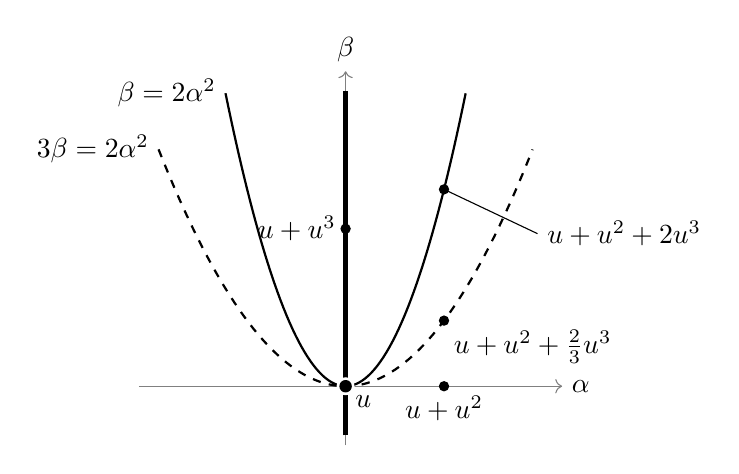
\begin{tikzpicture}[scale=1.25]
 \draw[->,gray] (-2.1,0) -- (2.2,0) node[right,black] {$\alpha$};
 \draw[->,gray] (0,-0.6) -- (0,3.2) node[above,black] {$\beta$};
 \draw[line width=1.6pt] (0,-0.5) -- (0,3.0);
 \draw[thick,domain=-1.22:1.22,samples=80] plot (\x,{2*\x*\x});
 \draw[thick,dashed,domain=-1.9:1.9,samples=80] plot (\x,{2*\x*\x/3});
 \node[left] at (-1.22,2.98) {$\beta=2\alpha^2$};
 \node[left] at (-1.9,2.41) {$3\beta=2\alpha^2$};
 \fill[white] (0,0) circle (2.6pt); \fill (0,0) circle (1.8pt);
 \node[below right] at (0,0) {$u$};
 \fill (0,1.6) circle (1.5pt) node[left] {$u+u^3$};
 \fill (1,0) circle (1.5pt) node[below] {$u+u^2$};
 \fill (1,2) circle (1.5pt);
 \draw[thin] (1,2) -- (1.95,1.55) node[right] {$u+u^2+2u^3$};
 \fill (1,0.6667) circle (1.5pt) node[below right] {$u+u^2+\frac23u^3$};
\end{tikzpicture}
\caption{The coefficient plane for $f=u+\alpha u^2+\beta u^3$. Scaling
moves points along the parabolas $\beta=\lambda\alpha^2$ and along the
$\beta$-axis. For trees of maximum degree at most three the Hilbert series
depends only on the cell (Theorem~\ref{thm:subcubic-strata}): the origin
$f=u$; the punctured $\beta$-axis (thick); the punctured parabola
$\beta=2\alpha^2$, where $[u^3]f^{-1}=0$; and the open complement. The
dashed parabola $3\beta=2\alpha^2$ contains the degree-three truncations
of the exponentials $(e^{cu}-1)/c$, for example $u+u^2+\frac23u^3$ for $c=2$. It
lies in the generic cell for trees but is exceptional for some graphs with
cycles (Proposition~\ref{prop:small-parameter-strata},
Table~\ref{tab:profile-G8} and Section~\ref{sec:exceptional-functions}).}
\label{fig:parameter-plane}
\end{figure}

\begin{table}[htbp]
\centering\renewcommand{\arraystretch}{1.15}
\begin{tabular}{lll}\toprule
$f$ & $\mathrm D_6=T(1,1,3)$ & $\mathrm E_6=T(1,2,2)$\\\midrule
$u$ & $(1+t)^5$ & $(1+t)^5$\\
$u+u^3$ & $1+6t+12t^2+10t^3+3t^4$ & $1+6t+12t^2+10t^3+3t^4$\\
$u+u^2$ & $1+6t+16t^2+9t^3$ & $1+6t+16t^2+9t^3$\\
$u+u^2+2u^3$ & $1+6t+16t^2+9t^3$ & $1+6t+15t^2+10t^3$\\\bottomrule
\end{tabular}
\caption{Hilbert series of the trees $\mathrm D_6$ and $\mathrm E_6$, with arms of
lengths $(1,1,3)$ and $(1,2,2)$, on the four cells of
Theorem~\ref{thmB}(ii). For $f=u+u^3$ the two filtered algebras are
even isomorphic (Proposition~\ref{prop:D6E6}); for $\alpha\ne0$ they are
not (Theorem~\ref{th:Isom-f}). Only $\mathrm E_6$, which has a trivalent vertex
with two non-leaf neighbors, detects the cell $\beta=2\alpha^2$.}
\label{tab:D6E6}
\end{table}

\subsection{Which trees detect the exceptional subcubic cell?}
\label{sec:subcubic-visibility}

An individual tree need not distinguish all four cells of
Theorem~\ref{thm:subcubic-strata}. We now characterize when the two
nonzero-quadratic cells have different Hilbert series. For a subcubic tree
$T$, write
\[
H_T^{\mathrm g}=\hs_T^{\,u+u^2},\qquad
H_T^{\mathrm s}=\hs_T^{\,u+u^2+2u^3}.
\]
The superscripts denote the generic and special nonzero-quadratic cells.
At a vertex of $T$, each incident branch is considered with that vertex
as its open leaf endpoint. Its boundary-state sum is the element of
$\mathcal S$ defined in~\eqref{eq:boundary-state-sum}; it does not
include the generator of the vertex at which the branches meet.

\begin{proposition}[Graphical detection of the exceptional cell]
\label{prop:subcubic-visibility}
Let $T$ be a finite tree of maximum degree at most three. The following
conditions are equivalent:
\begin{enumerate}[(i)]
\item $H_T^{\mathrm g}\ne H_T^{\mathrm s}$;
\item $T$ has a trivalent vertex with at least two neighbors that are not
leaves;
\item $T$ contains as a subtree the six-vertex tree with arm lengths
$1,2,2$ (the tree of type $\mathrm E_6$).
\end{enumerate}
Moreover,
\begin{equation}\label{eq:subcubic-visibility-defect}
H_T^{\mathrm g}-H_T^{\mathrm s}=t^2(1-t)C_T(t),
\qquad C_T(t)\in\Z_{\ge0}[t].
\end{equation}
If the equivalent conditions hold, then $C_T(0)=1$; in particular,
\begin{equation}\label{eq:subcubic-quadratic-drop}
[t^2]H_T^{\mathrm g}-[t^2]H_T^{\mathrm s}=1.
\end{equation}
\end{proposition}

\begin{proof}
The equivalence of (ii) and (iii) follows by extending two of the three
edges at the trivalent vertex by one edge each. In a tree the additional
vertices are distinct and introduce no further edges.

Let $\mathsf B_{\mathrm g}$ and $\mathsf B_{\mathrm s}$ be the two
branching operations in~\eqref{eq:subcubic-branching-table}, and put
$\Delta\mathsf B=\mathsf B_{\mathrm g}-\mathsf B_{\mathrm s}$.
Their only nonzero differences on unordered pairs of basis states are
\begin{align*}
\Delta\mathsf B(e_1,e_2)
 &=e_3-(1+t)e_2+te_1,\\
\Delta\mathsf B(e_2,e_2)
 &=e_3-e_2+t^2(e_0-e_1).
\end{align*}
Since $\mathsf E(e_i,e_j)=1+t^{\min(i,j)}$ by
\eqref{eq:edge-closing}, substitution gives the symmetric identity
\begin{equation}\label{eq:subcubic-local-defect}
\mathsf E\bigl(\Delta\mathsf B(e_i,e_j),e_k\bigr)
=\begin{cases}
 t^2(1-t),&\text{if the multiset }\{i,j,k\}\text{ is }
                   \{1,2,2\}\text{ or }\{2,2,2\},\\
 0,&\text{otherwise},
\end{cases}
\qquad 0\le i,j,k\le3.
\end{equation}
Thus the three incident branches can be treated symmetrically, although
the branching notation designates one outgoing edge.

For this proof, assign to each trivalent vertex a function
$f_v\in\{f_{\mathrm g},f_{\mathrm s}\}$, where
$f_{\mathrm g}=u+u^2$ and $f_{\mathrm s}=u+u^2+2u^3$. These two
functions give the same generators at leaves and bivalent vertices.
The local construction~\eqref{eq:branch-local-columns} still applies,
because its new generator depends only on the choice at that vertex.
Every branch is represented by a polynomial combination of $e_0,e_1,e_2,e_3$
with nonnegative integer coefficients, by induction from $e_1$ using the
path-extension and branching tables. Replacing $f_v=f_{\mathrm s}$ by
$f_v=f_{\mathrm g}$ at a single trivalent vertex, while fixing all
other choices, therefore changes the closed Hilbert series by
\[
t^2(1-t)C_v(t),\qquad C_v(t)\in\Z_{\ge0}[t],
\]
by~\eqref{eq:subcubic-local-defect}. Summing over a succession of such
replacements proves~\eqref{eq:subcubic-visibility-defect}.

First assign $f_{\mathrm s}$ to every trivalent vertex. The constant
term of the boundary-state sum of a branch is $e_1$ if the branch is a
single edge and $e_2$ otherwise. Here the constant term
means evaluation at $t=0$ in the state module. Indeed, the special table
has $T e_1|_{t=0}=T e_2|_{t=0}=e_2$ and
$\mathsf B_{\mathrm s}(e_i,e_j)|_{t=0}=e_2$ for $i,j\in\{1,2\}$.
If $v$ satisfies (ii), at least two of its incident boundary-state sums have constant
term $e_2$, and the third has constant term $e_1$ or $e_2$. Replace
$f_v$ by $f_{\mathrm g}$ first. Equation~\eqref{eq:subcubic-local-defect} gives $C_v(0)=1$.
The nonnegative later contributions cannot cancel it, proving (i).
Conversely, if (ii) fails, every trivalent vertex has at least two leaf
neighbors. At any replacement two of its boundary-state sums are exactly $e_1$, so
\eqref{eq:subcubic-local-defect} gives zero, regardless of the third
boundary-state sum. Hence $H_T^{\mathrm g}=H_T^{\mathrm s}$.

It remains to show that no later replacement contributes to the quadratic
coefficient if $f_v$ is replaced first at a vertex satisfying (ii).
At an intermediate stage, some trivalent vertices carry $f_{\mathrm g}$
and the others still carry $f_{\mathrm s}$. We first determine the
constant terms of the boundary-state sums for these assignments. At
$t=0$ the bivalent rule sends $e_1,e_2$ to $e_2$ and
$e_3$ to $e_3$, while both branching tables send $(e_1,e_1)$ to $e_2$,
send $(e_i,e_3)$ to $e_3$ for $i\ge1$, and send $(e_1,e_2)$ and $(e_2,e_2)$
to $e_3$ in the generic table and to $e_2$ in the special one. By
induction from the leaves, for every such assignment the boundary-state
sum of a branch has a single basis state as its constant term: $e_1$
if the branch is a single edge ending in a leaf, and $e_2$ or $e_3$
otherwise.

Now let $w\ne v$ be another trivalent vertex. By (ii), at most one
neighbor of $v$ is a leaf. Hence, of the two branches at $v$ that do not
contain $w$, at least one has more than one edge, and their constant terms are
$(e_i,e_j)$ with $i,j\in\{1,2,3\}$, not both equal to $1$. Since
$f_v=f_{\mathrm g}$, the table for $f_{\mathrm g}$ sends each such pair
to $e_3$ at $t=0$. Along the path from $v$ to $w$, the bivalent
path-extension rule preserves $e_3$ at $t=0$,
and at an intervening trivalent vertex either table sends $(e_3,e_j)$,
$j\in\{1,2,3\}$, to $e_3$ at $t=0$. Thus, when $f_w$ is replaced by
$f_{\mathrm g}$, one of its three incident boundary-state sums has
constant term $e_3$. Since
\eqref{eq:subcubic-local-defect} is trilinear and vanishes whenever one
index equals $3$, the contribution of degree $2$ comes only from the
constant states and is equal to zero, that is, $C_w(0)=0$.
Consequently $C_T(0)=1$, proving~\eqref{eq:subcubic-quadratic-drop}.
\end{proof}

For the smallest tree satisfying these conditions, the difference is
exactly $t^2(1-t)$:
\[
H_{T(1,2,2)}^{\mathrm g}=1+6t+16t^2+9t^3,\qquad
H_{T(1,2,2)}^{\mathrm s}=1+6t+15t^2+10t^3.
\]
In contrast, the tree with arm lengths $1,1,r$ does not distinguish the
two cells for any $r\ge1$. Other pairs of cells can also merge for a
particular tree. For example the star $S_4$ has only two strata
(Section~\ref{sec:small-strata}).

\subsection{Trees of maximum degree four}
\label{sec:D4-cells}

For $D=4$ the procedure of Theorem~\ref{thm:uniform-tree-strata}
gives eight parts distinguished by three inverse coefficients. Writing
$g=f^{-1}$ and $g_j=[u^j]g$, we have, by~\eqref{eq:inverse-jet},
\[
[u^2]g=-\alpha,\qquad [u^3]g=2\alpha^2-\beta,\qquad [u^4]g=-5\alpha^3+5\alpha\beta-\gamma.
\]

\begin{theorem}[The eight cells for $D=4$; computer-assisted]
\label{thm:D4-strata}
Let $f=u+\alpha u^2+\beta u^3+\gamma u^4$. For every tree $T$ of maximum
degree at most four, $\hs_T^f$ depends only on which of the coefficients
$[u^2]f^{-1}$, $[u^3]f^{-1}$, $[u^4]f^{-1}$ vanish. All eight vanishing
patterns occur, and any two of them are distinguished by some tree with at
most ten vertices.
\end{theorem}

The cells are listed in Table~\ref{tab:D4-cells}. For $D=3$ the
coefficient $[u^4]f^{-1}$ plays no role, and the statement reduces to
Theorem~\ref{thm:subcubic-strata}.

\begin{table}[htbp]
\centering\renewcommand{\arraystretch}{1.15}
\begin{tabular}{clll}\toprule
Cell & Vanishing coefficients of $g$ & Representative & Conditions on $(\alpha,\beta,\gamma)$\\\midrule
1 & $[u^2],[u^3],[u^4]$ & $u$ & $\alpha=\beta=\gamma=0$\\
2 & $[u^2],[u^3]$ & $u+u^4$ & $\alpha=\beta=0$, $\gamma\ne0$\\
3 & $[u^2],[u^4]$ & $u+u^3$ & $\alpha=\gamma=0$, $\beta\ne0$\\
4 & $[u^2]$ & $u+u^3+u^4$ & $\alpha=0$, $\beta\gamma\ne0$\\
5 & none & $u+u^2$ & $\alpha\ne0$, $\beta\ne2\alpha^2$, $\gamma\ne5\alpha\beta-5\alpha^3$\\
6 & $[u^3]$ & $u+u^2+2u^3$ & $\alpha\ne0$, $\beta=2\alpha^2$, $\gamma\ne5\alpha^3$\\
7 & $[u^4]$ & $u+u^2+u^3$ & $\alpha\ne0$, $\beta\ne2\alpha^2$, $\gamma=5\alpha\beta-5\alpha^3$\\
8 & $[u^3],[u^4]$ & $u+u^2+2u^3+5u^4$ & $\alpha\ne0$, $\beta=2\alpha^2$, $\gamma=5\alpha^3$\\\bottomrule
\end{tabular}
\caption{The eight cells of Theorem~\ref{thm:D4-strata}, where
$g=f^{-1}$. The representative of cell~8 is the inverse of $u-u^2$
modulo $u^5$.}
\label{tab:D4-cells}
\end{table}

The following trees distinguish the cells. Their Hilbert series are
computed by the boundary-state algorithm. The path with two edges separates
$\alpha=0$ from $\alpha\ne0$ (series $1+2t+t^2$ and $1+3t$, respectively).
Among the cells with $\alpha=0$, the star $S_4$ separates cells $3,4$ from
$1,2$, the star $S_5$ separates cell~$2$ from cell~$1$, and the
nine-vertex tree with a vertex of degree four adjacent to two leaves and
to two vertices carrying two leaves each separates cell~$4$ from cell~$3$:
\[
1+9t+37t^2+89t^3+88t^4+31t^5+t^6\quad\text{against}\quad
1+9t+37t^2+88t^3+89t^4+31t^5+t^6.
\]
Among the cells with $\alpha\ne0$, the tree $\mathrm E_6$ separates cells $6,8$
from cells $5,7$ (Table~\ref{tab:D6E6}). The star $S_5$ with one edge
subdivided separates cell~$8$ from cells $5,6,7$, with series
$1+6t+15t^2+10t^3$ against $1+6t+16t^2+9t^3$. The ten-vertex tree with edges
\[
12,\ 13,\ 14,\ 15,\ 26,\ 27,\ 28,\ 39,\ 4\,10,
\]
has two adjacent vertices of degree four. It separates cell~$5$ from
cell~$7$, in the following order:
\[
1+10t+47t^2+136t^3+234t^4+84t^5\quad\text{against}\quad
1+10t+47t^2+135t^3+235t^4+84t^5.
\]

\begin{proof}[Proof of Theorem~\ref{thm:D4-strata}]
We follow the proof of Theorem~\ref{thm:uniform-tree-strata}, keeping
track of the parameters. On $\alpha\ne0$ normalize $\alpha=1$ by
scaling and write $f=u+u^2+bu^3+cu^4$.

\emph{Iteration of the local branching rules.} Start from the leaf
state, of gap one. For every
multiset of at most three incoming gaps that has occurred, form the local
columns~\eqref{eq:branch-local-columns} and compute the
ranks~\eqref{eq:local-intersection-rank} by exact elimination over
$\mathbb{Q}(b,c)$, recording every factor by which a pivot is divided.
Add the outgoing gaps and repeat until no new gap appears. This gives the
gaps $0,\ldots,4$, fifty-five local tables, and only three nonconstant
pivot factors:
\[
b-2,\qquad c-5b+5,\qquad c-b^2-b+1 .
\]
The first two are $-[u^3]g$ and $-[u^4]g$.

\emph{Recomputation on the curves.} Over the function field of each
curve, repeat this iteration from the original generators, again
recording every pivot factor. On $b=2$ and on $c=5b-5$ some tables
change; on $c=b^2+b-1$ (equivalently $g_2g_4=g_3^2$) all tables agree
with the generic ones. In each of the three calculations the only pivot
factor is $c-5$ (on $b=2$) or $b-2$ (on the other two curves), and it
vanishes on the curve only at $(b,c)=(2,5)$. As in
Appendix~\ref{app:certificates}, the tables of each curve therefore hold
at all its points except $(2,5)$.

The common point $(2,5)$ is a separate part of the partition. Before
normalization it consists of
$f=u+\alpha u^2+2\alpha^2u^3+5\alpha^3u^4$, $\alpha\ne0$,
a single scaling orbit. Constancy on this part follows from scaling,
not from specializing the generic curve tables.

\emph{The locus $\alpha=0$.} Scaling, after a field extension, reduces
it to $f=u+u^3+\gamma u^4$, to $u+u^4$, and to $u$. Over
$\mathbb{Q}(\gamma)$ the first family has the single pivot factor
$\gamma$, so its local tables are constant for $\gamma\ne0$.
The specialization $\gamma=0$, represented by $u+u^3$, and the
remaining cases $u+u^4$ and $u$ each form a single scaling orbit.
Constancy on each of these parts again follows from scaling.

Field extensions do not change ranks, and Hilbert functions are constant
on scaling orbits. Hence all local tables are constant on each of the
eight cells, and by induction over the tree and the closing
rule~\eqref{eq:edge-closing} so is every Hilbert series of a tree with
$\Delta\le4$. The separating trees above were found by evaluating all
trees with $\Delta\le4$ and at most ten vertices at one point of each cell.
All arithmetic is exact. The corresponding scripts are described in
Appendix~\ref{app:certificates}.
\end{proof}

\begin{remark}[Degree five]\label{rem:D5}
The pattern of Theorem~\ref{thm:D4-strata} does not persist. For $D=5$,
with $f=u+u^2+bu^3+cu^4+du^5$, iteration of the local branching rules
over $\mathbb{Q}(b,c,d)$ produces the gaps $0,\ldots,5$, two hundred
and nine local tables, and nine pivot hypersurfaces. At a general point of each hypersurface, recomputation leaves all tables
unchanged for four and changes some tables for five. Each of the latter
five is detected generically by a tree. Writing
$g_k=[u^k]f^{-1}$:
\begin{enumerate}[(a)]
\item $g_3=0$, by $\mathrm E_6$;
\item $g_4=0$, by the ten-vertex tree above;
\item $g_5=0$, first by a tree with fourteen vertices, which has two
adjacent vertices of degree five;
\item the \emph{star locus} $\alpha^2\delta-3\alpha\beta\gamma+2\beta^3=0$,
by the star $S_6$, whose series drops from $1+6t+16t^2+9t^3$ to
$1+6t+15t^2+10t^3$;
\item the Hankel surface $g_3g_5=g_4^2$, by the tree with a vertex of
degree five carrying two leaves and three arms of length two, whose series
drops from $1+9t+37t^2+93t^3+116t^4$ to $1+9t+37t^2+92t^3+117t^4$.
\end{enumerate}
The star locus follows from a $3\times3$ determinant. By Theorem~\ref{thm:star-hilb} the
series of $S_6$ is determined by the ranks $r^f_{5,d}$, and $r^f_{5,2}$
drops below six exactly when $f$, $xf$ and $f^2$ are linearly dependent
in $\K[x]/(x^6)$ modulo $1,x,x^2$. The corresponding $3\times3$
determinant is $\alpha(\alpha^2\delta-3\alpha\beta\gamma+2\beta^3)$.
This locus is invariant under $f\mapsto f^{-1}$, as
Corollary~\ref{cor:star-inversion} requires, and it contains the inverse
quadratics and $u/(1-u)$. It is not, however, the vanishing locus of an individual coefficient of
$f^{-1}$. We have not recomputed the intersections of these surfaces or
the locus $\alpha=0$, so the complete partition for $D=5$ is open
(Section~\ref{sec:outlook}). The smallest tree detecting $g_5=0$ was found
by an exhaustive search over trees with $\Delta\le5$ and at most fourteen
vertices.
\end{remark}

\subsection{Distinguished functions and graph-dependent exceptionality}
\label{sec:exceptional-functions}

A parameter $f$ is \emph{Hilbert-exceptional} for $G$ if $\hs_G^f$
differs from the generic series of
Theorem~\ref{thm:determinantal-strata}(ii). The exponential and inverse
polynomials are distinguished for different elementary reasons.

Let $g=f^{-1}$. On each connected component the defining relations give
\begin{equation}\label{eq:inverse-component-relation}
\sum_vg(Y_v)=0.
\end{equation}
If $g$ is a polynomial of degree $s$, this is a relation of filtration
degree at most $s$, regardless of the vertex degrees. In particular,
$g(u)=u+cu^2$ gives $\sum_vY_v+c\sum_vY_v^2=0$.
Whether such a short relation lowers a Hilbert value depends on the
graph. For the inverse-quadratic
truncation through degree three on subcubic trees,
Proposition~\ref{prop:subcubic-visibility}
gives the exact test.

\begin{proposition}[Inverse degree and boundary gaps]
\label{prop:inverse-degree-gap}
If $f^{-1}$ is a polynomial of degree at most $s$, then every boundary
state of every marked graph satisfies $q-p\le s$.
In particular, for an inverse quadratic $f^{-1}(u)=u+cu^2$, $c\ne0$,
every long-neck family with arbitrary side graphs satisfies
\begin{equation}\label{eq:inverse-quadratic-neck}
L(H_n)=0\qquad(n\ge5).
\end{equation}
For a fixed graph, the same gap bound holds whenever the relevant
truncation of $f^{-1}$ through the maximum vertex degree has degree at most $s$.
\end{proposition}
\begin{proof}
At a marked leaf $a$ with edge variable $r$, the identity
$X_a=-\sum_{v\ne a}X_v=-\sum_{v\ne a}g(Y_v)$ gives $r\in P_s$.
Multiplying a lift of $u\in Q_i$ by $r$ then gives
$ru\in P_{i+s}$, so $Q_i\subseteq R_{i+s}$.
The bound follows from a simultaneous adapted basis.
For an inverse quadratic, both side graphs in the neck construction
have no gap greater than two. Theorem~\ref{thm:longneck} gives
\eqref{eq:inverse-quadratic-neck}.
\end{proof}

For the exponential parameter $f(u)=(\exp(cu)-1)/c$, $c\ne0$, the
simplification instead concerns addition:
\[
1+cf(x+x')=(1+cf(x))(1+cf(x')).
\]
Internal edge contributions cancel across a cut, so
\begin{equation}\label{eq:exponential-cut-relations}
\left(\prod_{v\in I}(1+cY_v)-1\right)^{D_I+1}=0,
\qquad \prod_{v\in V(C)}(1+cY_v)=1
\end{equation}
for each connected component $C$. These are the multiplicative cut
relations of \cite[Theorem~3]{NSh}, after normalization. The inverse
series is logarithmic, not polynomial. At a square-zero boundary $r$,
\[
f(x+r)=f(x)+r(1+cf(x)),
\]
so coefficient extraction gives $\delta_r(P_i)\subseteq Q_i$ and
hence $R_i\subseteq Q_i$. All exponential boundary gaps are therefore
nonnegative, rather than bounded above by two.

The contrast is already visible in the examples. The normalized cubic
ratio $\lambda=\beta/\alpha^2$ is $2$ for the inverse quadratic and
$2/3$ for the exponential (Figure~\ref{fig:parameter-plane}). The first
is detected by subcubic trees. The exponential, in contrast, lies in the
generic cell for every tree of maximum degree at most four: its inverse
$\log(1+u)$ has $[u^3]=1/3$ and $[u^4]=-1/4$, so
Theorem~\ref{thm:D4-strata} applies. It also avoids the five loci of
Remark~\ref{rem:D5}. By Proposition~\ref{prop:star-exponential} and
Corollary~\ref{cor:star-inversion}, the exponential is generic on every
star, while an inverse quadratic is exceptional on every star with at
least six vertices.

The exponential is exceptional, however, for small graphs with cycles.
The first examples are the multigraphs of \cite[Example~2]{NSh}: for the
$4$-cycle with two opposite edges doubled and for the $4$-cycle with two
adjacent edges doubled, the exponential gives
$1+4t+10t^2+14t^3+3t^4$ and $1+4t+10t^2+15t^3+2t^4$, while the generic
series are $1+4t+10t^2+15t^3+2t^4$ and $1+4t+10t^2+16t^3+t^4$. We
confirmed these values by exact computation.
Besides the doubled triangle (Proposition~\ref{prop:small-parameter-strata})
and the unicycles $G8$ (Table~\ref{tab:profile-G8}), four simple graphs
with five vertices and maximum degree three have this property: the
triangle with a path of length two attached at one endpoint, the house,
the kite ($K_4$ minus an edge, with a leaf edge) and $K_{2,3}$. For the
first of them the series at $u+u^2$ and at $e^u-1$ are
\[
1+5t+13t^2+8t^3+t^4\qquad\text{and}\qquad 1+5t+13t^2+7t^3+2t^4.
\]
Six graphs with five vertices and $\Delta=4$ are added in
Proposition~\ref{prop:exp-small}.
For \cite[Problem~3]{NSh}, which asks for which graphs the exponential
is generic, the answer therefore depends on the graph: it is affirmative
for stars and for all trees with $\Delta\le4$, and negative for these
graphs with cycles. Functional
identities single out parameter loci, but the graph determines which of
them are Hilbert-exceptional.

\begin{remark}[Complete profiles of small graphs]
\label{rem:small-complete-profiles}
For each of the eighteen graphs of maximum degree three with four or
five vertices in Tables~B1--B3 of \cite[\texttt{tables/}]{Cert}, the complete
Hilbert partition of the cubic parameter plane was computed exactly: the
generic ranks over $\mathbb{Q}(\lambda)$ with all pivot factors recorded,
then a recomputation over the residue field of every factor, and
separately the two orbits with $\alpha=0$. In every case the only
exceptional values are $\lambda=2$ (for twelve of the graphs) and
$\lambda=2/3$ (for six graphs, all of which contain a cycle and are also
exceptional at $\lambda=2$). On these graphs the inverse quadratic and the
exponential therefore give the only exceptional parameters with
$\alpha\ne0$, after truncation through degree three. The full profiles
are listed in those tables.
\end{remark}

\subsection{Universal Hilbert equivalence and exact collisions}
\label{sec:universal-collisions}

Recall that universal Hilbert equivalence means equality of the
nondegenerate profiles at the same parameter. We compare the profiles
on a common space $\cA_D$, with
$D\ge\max\{1,\Delta(G),\Delta(G')\}$.

\begin{proposition}[A determinantal criterion]\label{prop:universal-minors}
Over an algebraically closed field, universal Hilbert equivalence is
equivalent to
\begin{equation}\label{eq:universal-radicals}
\sqrt{I_{r+1}(M_{G,i})}=\sqrt{I_{r+1}(M_{G',i})}
\quad\text{for every }i,r.
\end{equation}
Only finitely many $i,r$ are needed.
\end{proposition}
\begin{proof}
We view the entries of $M_{G,i}$ and $M_{G',i}$ as polynomials on the common space $\cA_D$. The ones in $M_{G,i}$ involve only $a_j$ with
$j\le\Delta(G)$. By~\eqref{eq:universal-rank}, the zero set of
$I_{r+1}(M_{G,i})$ in $\cA_D(\K)$ is the set of $f$ with
$\dim\CC_G^{f,i}\le r$. The Hilbert series $\hs^f_G$ is determined by
the cumulative dimensions $\dim\CC_G^{f,i}$, $i\ge0$, and conversely.
Hence $\hs_G^f=\hs_{G'}^f$ for all $f$ if and only if, for every $i$
and $r$, the two determinantal loci have the same $\K$-points. Over an
algebraically closed field this is equivalent to~\eqref{eq:universal-radicals},
by the Nullstellensatz. Let $N$ and $N'$ be the numbers of non-loop edges of $G$ and $G'$.
For $i\ge\max(N,N')$ both cumulative dimensions are the total
dimensions, so these conditions coincide with the one for
$i=\max(N,N')$. For $r\ge\max(\dim\CC_G,\dim\CC_{G'})$ both ideals are
zero. Thus only finitely many pairs $(i,r)$ give distinct conditions.
\end{proof}

The following examples show that even this pointwise profile is not a
complete invariant. Use the notation $ij=\{i,j\}$ in the edge sets
\begin{equation}\label{eq:collision-edge-lists}
\begin{aligned}
G8_1&=\{12,23,34,41,15,56,27,38\},&
G8_2&=\{12,23,34,41,15,56,27,48\},\\
T1_1&=\{12,23,34,45,56,27,48,29,8\,10\},&
T1_2&=\{12,23,34,45,56,27,48,29,1\,10\},\\
T2_1&=\{12,23,34,45,56,27,38,89,9\,10\},&
T2_2&=\{12,23,34,45,56,27,38,19,9\,10\},\\
T3_1&=\{12,13,14,25,26,37,38,49,9\,10\},&
T3_2&=\{12,13,14,25,26,37,38,59,9\,10\}.
\end{aligned}
\end{equation}
The notation $8\,10$, for example, denotes the edge $\{8,10\}$.
The graphs are drawn in Figure~\ref{fig:collisions}.

\begin{figure}[htbp]
\centering
\tikzset{cv/.style={circle,fill,inner sep=1.2pt},
  lab/.style={font=\tiny,inner sep=1.5pt}}
\begin{tabular}{c@{\qquad}c}
\begin{tikzpicture}[scale=.62]
 \foreach \n/\x/\y/\p in {1/0/0/below,2/1/0/below,3/1/1/above,4/0/1/above,5/-1/0/below,6/-2/0/below,7/2/0/below,8/2/1/above}
   \node[cv,label={[lab]\p:\n}] (v\n) at (\x,\y) {};
 \draw (v1)--(v2)--(v3)--(v4)--(v1) (v1)--(v5)--(v6) (v2)--(v7) (v3)--(v8);
\end{tikzpicture}
&
\begin{tikzpicture}[scale=.62]
 \foreach \n/\x/\y/\p in {1/0/0/below,2/1/0/below,3/1/1/above,4/0/1/above,5/-1/0/below,6/-2/0/below,7/2/0/below,8/-1/1/above}
   \node[cv,label={[lab]\p:\n}] (v\n) at (\x,\y) {};
 \draw (v1)--(v2)--(v3)--(v4)--(v1) (v1)--(v5)--(v6) (v2)--(v7) (v4)--(v8);
\end{tikzpicture}
\\[-1pt]
$G8_1$ & $G8_2$\\[6pt]
\begin{tikzpicture}[scale=.62]
 \foreach \n/\x/\y/\p in {1/0/0/below,2/1/0/below right,3/2/0/below,4/3/0/below,5/4/0/below,6/5/0/below,7/1/1/above,9/1/-1/below,8/3/1/right,10/3/2/right}
   \node[cv,label={[lab]\p:\n}] (v\n) at (\x,\y) {};
 \draw (v1)--(v2)--(v3)--(v4)--(v5)--(v6) (v2)--(v7) (v2)--(v9) (v4)--(v8)--(v10);
\end{tikzpicture}
&
\begin{tikzpicture}[scale=.62]
 \foreach \n/\x/\y/\p in {10/-1/0/below,1/0/0/below,2/1/0/below right,3/2/0/below,4/3/0/below,5/4/0/below,6/5/0/below,7/1/1/above,9/1/-1/below,8/3/1/right}
   \node[cv,label={[lab]\p:\n}] (v\n) at (\x,\y) {};
 \draw (v10)--(v1)--(v2)--(v3)--(v4)--(v5)--(v6) (v2)--(v7) (v2)--(v9) (v4)--(v8);
\end{tikzpicture}
\\[-1pt]
$T1_1$ & $T1_2$\\[6pt]
\begin{tikzpicture}[scale=.62]
 \foreach \n/\x/\y/\p in {1/0/0/below,2/1/0/below,3/2/0/below,4/3/0/below,5/4/0/below,6/5/0/below,7/1/1/left,8/2/1/right,9/2/2/right,10/2/3/right}
   \node[cv,label={[lab]\p:\n}] (v\n) at (\x,\y) {};
 \draw (v1)--(v2)--(v3)--(v4)--(v5)--(v6) (v2)--(v7) (v3)--(v8)--(v9)--(v10);
\end{tikzpicture}
&
\begin{tikzpicture}[scale=.62]
 \foreach \n/\x/\y/\p in {1/0/0/below,2/1/0/below,3/2/0/below,4/3/0/below,5/4/0/below,6/5/0/below,7/1/1/right,8/2/1/right,9/0/1/left,10/0/2/left}
   \node[cv,label={[lab]\p:\n}] (v\n) at (\x,\y) {};
 \draw (v1)--(v2)--(v3)--(v4)--(v5)--(v6) (v2)--(v7) (v3)--(v8) (v1)--(v9)--(v10);
\end{tikzpicture}
\\[-1pt]
$T2_1$ & $T2_2$\\[6pt]
\begin{tikzpicture}[scale=.62]
 \foreach \n/\x/\y/\p in {1/0/0/below,2/-1.2/0/below,3/1.2/0/below,4/0/1/right,9/0/2/right,10/0/3/right,5/-2/.7/left,6/-2/-.7/left,7/2/.7/right,8/2/-.7/right}
   \node[cv,label={[lab]\p:\n}] (v\n) at (\x,\y) {};
 \draw (v2)--(v1)--(v3) (v1)--(v4)--(v9)--(v10) (v2)--(v5) (v2)--(v6) (v3)--(v7) (v3)--(v8);
\end{tikzpicture}
&
\begin{tikzpicture}[scale=.62]
 \foreach \n/\x/\y/\p in {1/0/0/below,2/-1.2/0/below,3/1.2/0/below,4/0/1/right,5/-1.2/1/right,9/-1.2/2/right,10/-1.2/3/right,6/-2/-.7/left,7/2/.7/right,8/2/-.7/right}
   \node[cv,label={[lab]\p:\n}] (v\n) at (\x,\y) {};
 \draw (v2)--(v1)--(v3) (v1)--(v4) (v2)--(v5)--(v9)--(v10) (v2)--(v6) (v3)--(v7) (v3)--(v8);
\end{tikzpicture}
\\[-1pt]
$T3_1$ & $T3_2$
\end{tabular}
\caption{The four pairs of universally Hilbert equivalent graphs of
Proposition~\ref{prop:universal-collisions}, numbered as
in~\eqref{eq:collision-edge-lists}. The two graphs in each row are not
isomorphic. In $G8_1$ there are two leaves attached to adjacent vertices and in $G8_2$ there are none.
In $T1_1$ the degree-four vertex has three leaf neighbors and in $T1_2$ it has only two.
In $T2_1$ there is a vertex with two attached leaves and in $T2_2$ there is no such vertex.
 In $T3_1$ there are two vertices with two leaves attached and $T3_2$ has only one such vertex.}
\label{fig:collisions}
\end{figure}

\begin{proposition}[Universal collisions]\label{prop:universal-collisions}
Each pair in~\eqref{eq:collision-edge-lists} consists of nonisomorphic
universally Hilbert equivalent graphs over every characteristic-zero
field. Their complete pointwise Hilbert profiles are given in
Tables~\ref{tab:profile-G8}--\ref{tab:profile-T3}.
Unspecified coefficients in the conditions are arbitrary, and all
coefficients beyond the maximum vertex degree are irrelevant.
\end{proposition}

\begin{table}[htbp]
\centering\renewcommand{\arraystretch}{1.17}
\begin{tabular}{ll}\toprule
Condition on $f=u+\alpha u^2+\beta u^3$&Hilbert function of $G8_1,G8_2$\\\midrule
$\alpha=\beta=0$&$(1,7,24,50,66,55,28,8,1)$\\
$\alpha=0,\ \beta\ne0$&$(1,8,32,72,81,40,6)$\\
$\alpha\ne0,\ \beta=2\alpha^2$&$(1,8,31,77,111,12)$\\
$\alpha\ne0,\ 3\beta=2\alpha^2$&$(1,8,32,84,107,8)$\\
$\alpha\ne0,\ \beta\ne2\alpha^2,\ 3\beta\ne2\alpha^2$
 &$(1,8,32,84,111,4)$\\\bottomrule
\end{tabular}
\caption{Complete nondegenerate Hilbert profile of the eight-vertex unicycle pair.}
\label{tab:profile-G8}
\end{table}

\begin{table}[htbp]
\centering\renewcommand{\arraystretch}{1.17}
\begin{tabular}{ll}\toprule
Condition on $f=u+\alpha u^2+\beta u^3+\gamma u^4$&Hilbert function of $T1_1,T1_2$\\\midrule
$\alpha=\beta=\gamma=0$&$(1,9,36,84,126,126,84,36,9,1)$\\
$\alpha=\beta=0,\ \gamma\ne0$&$(1,10,41,94,135,126,75,26,4)$\\
$\alpha=0,\ \beta\ne0$&$(1,10,47,115,157,122,51,9)$\\
$\alpha\ne0,\ \beta\ne2\alpha^2$&$(1,10,48,143,229,81)$\\
$\alpha\ne0,\ \beta=2\alpha^2,\ \gamma\ne5\alpha^3$&$(1,10,48,138,225,90)$\\
$\alpha\ne0,\ \beta=2\alpha^2,\ \gamma=5\alpha^3$&$(1,10,47,134,220,100)$\\\bottomrule
\end{tabular}
\caption{Complete nondegenerate Hilbert profile of the first ten-vertex tree pair.}
\label{tab:profile-T1}
\end{table}

\begin{table}[htbp]
\centering\renewcommand{\arraystretch}{1.17}
\begin{tabular}{ll}\toprule
Condition on $f=u+\alpha u^2+\beta u^3$&Hilbert function of $T2_1,T2_2$\\\midrule
$\alpha=\beta=0$&$(1,9,36,84,126,126,84,36,9,1)$\\
$\alpha=0,\ \beta\ne0$&$(1,10,44,106,150,126,60,14,1)$\\
$\alpha\ne0,\ \beta=2\alpha^2$&$(1,10,48,138,234,81)$\\
$\alpha\ne0,\ \beta\ne2\alpha^2$&$(1,10,49,146,225,81)$\\\bottomrule
\end{tabular}
\caption{Complete nondegenerate Hilbert profile of the second ten-vertex tree pair.}
\label{tab:profile-T2}
\end{table}

\begin{table}[htbp]
\centering\renewcommand{\arraystretch}{1.17}
\begin{tabular}{ll}\toprule
Condition on $f=u+\alpha u^2+\beta u^3$&Hilbert function of $T3_1,T3_2$\\\midrule
$\alpha=\beta=0$&$(1,9,36,84,126,126,84,36,9,1)$\\
$\alpha=0,\ \beta\ne0$&$(1,10,46,117,165,124,44,5)$\\
$\alpha\ne0,\ \beta=2\alpha^2$&$(1,10,48,138,234,81)$\\
$\alpha\ne0,\ \beta\ne2\alpha^2$&$(1,10,49,146,225,81)$\\\bottomrule
\end{tabular}
\caption{Complete nondegenerate Hilbert profile of the third ten-vertex tree pair. For
  $\alpha\ne0$ it agrees with Table~\ref{tab:profile-T2}. The only cell separating $T2$ from $T3$ is $\alpha=0\ne\beta$.}
\label{tab:profile-T3}
\end{table}

\begin{proof}
Each unicyclic graph has a unique four-cycle and a unique path of
length two attached to that cycle at one endpoint. Relative to this
attachment point, the other two leaf edges are
on adjacent cycle vertices for $G8_1$ and on the two neighbors for
$G8_2$. Thus they are nonisomorphic.
In $T1$, the degree-four and degree-three vertices are joined by a
length-two path. The remaining arm lengths are respectively
$(1,1,1)\mid(2,2)$ and $(2,1,1)\mid(2,1)$.
In $T2$, the two trivalent vertices are adjacent, with arm lengths
$(1,1)\mid(3,3)$ and $(1,3)\mid(1,3)$. In $T3_1$ two vertices have two
leaf neighbors each, whereas $T3_2$ has only one such vertex. These descriptions prove
nonisomorphism of the trees as well.

We specify the complete rank certificates, including all exceptional
loci, in Appendix~\ref{app:certificates}. For $T2$ and $\alpha\ne0$,
the calculation can also be displayed directly. An arm of length three
has states $T^2e_1=e_2+3te_1$. Write
$\mathsf B_{ij}=\mathsf B_\lambda(e_i,e_j)$. The two series are
\[
\mathsf E(\mathsf B_{11},\mathsf B_{22}+6t\mathsf B_{12}
                                      +9t^2\mathsf B_{11}),
\qquad
\mathsf E(\mathsf B_{12}+3t\mathsf B_{11},
          \mathsf B_{12}+3t\mathsf B_{11}).
\]
Symmetry and bilinearity reduce their equality to
$\mathsf E(\mathsf B_{11},\mathsf B_{22})
 =\mathsf E(\mathsf B_{12},\mathsf B_{12})$,
which follows by substituting either column of
\eqref{eq:subcubic-branching-table}. The resulting coefficients are given in Table~\ref{tab:profile-T2}.

For $T3$, Theorem~\ref{thm:subcubic-strata} reduces the claim to the four
representatives $u$, $u+u^3$, $u+u^2+2u^3$, $u+u^2$. The boundary-state
algorithm gives Table~\ref{tab:profile-T3} for both trees, and a direct
computation in the $512$-dimensional edge algebra confirms the three
values with $f\ne u$.

For $T1$, the local edge algebras have dimensions eight and sixteen.
With $\alpha=1$, exact elimination over $\mathbb{Q}(\beta,\gamma)$ excludes
only the three curves
\begin{equation}\label{eq:T1-pivot-curves}
\beta=2,\qquad \gamma=5\beta-5,\qquad
\gamma=\beta^2+\beta-1.
\end{equation}
Recomputing over the rational-function field of each curve records a
single further factor, $\gamma-5$ on $\beta=2$ and $\beta-2$ on the
other two curves. It vanishes on the curve only at the common point
$(\beta,\gamma)=(2,5)$, where we compute over $\mathbb{Q}$. Away from
this point the last two curves have the generic ranks, and the first
has the middle special row of Table~\ref{tab:profile-T1}.
On $\alpha=0$, scaling reduces to $\beta=1$ with $\gamma$ arbitrary,
$\beta=0,\gamma=1$, or the origin, with no further excluded factors.
This proves the whole table, not only its generic case.

For the unicycles, work in the $256$-dimensional edge algebra over
$\mathbb{Q}(\lambda)$, where $f=u+u^2+\lambda u^3$.
Over $\mathbb{Q}(\lambda)$, the matrix ranks give the Hilbert series
in the last row of Table~\ref{tab:profile-G8}. All factors excluded by
the elimination divide
\begin{equation}\label{eq:G8-pivot-polynomial}
(\lambda-2)(3\lambda-2)(3\lambda-4)(3\lambda-8)(3\lambda-10)
(9\lambda^2-30\lambda+8) (9\lambda^2-24\lambda-4).
\end{equation}
Starting again from the original generators, compute over the residue
field of every irreducible factor, including the two quadratic number
fields. Only $\lambda=2,2/3$ change the ranks. The cases
$\alpha=0,\beta=0$ and $\alpha=0,\beta\ne0$ are checked separately
over $\mathbb{Q}$ after scaling. This exhausts the parameter line.
All computations use exact arithmetic. Extending a  characteristic-zero field does not change the resulting ranks. The sums of the table entries are
$240$ for each unicycle and $512$ for each tree, as also required by
Theorem~\ref{th:forests}.
\end{proof}

We return to the degenerate functions of Section~\ref{sec:degenerate},
which enter \cite[Problem~5]{NSh}.

\begin{proposition}[Degenerate functions]\label{prop:degenerate-collisions}
\leavevmode
\begin{enumerate}[(i)]
\item The trees $T3_1$ and $T3_2$ have the same Hilbert series for every
polynomial $f$.
\item For $f=u^2$ the two graphs of the pairs $G8$, $T1$ and $T2$ have the
Hilbert functions
\[
(1,5,10,9,1),\ (1,5,10,10,1);\qquad
(1,5,11,10,4),\ (1,5,11,11,4);\qquad
(1,6,13,11,3),\ (1,6,13,12,3),
\]
respectively.
\end{enumerate}
In particular, the Hilbert series for all polynomials $f$ together do not
determine a tree up to isomorphism.
\end{proposition}
\begin{proof}
First subtract $f(0)$, which does not change the filtered algebra.
Both trees in $T3$ have maximum degree three. If $f'(0)\ne0$, part~(i)
is Proposition~\ref{prop:universal-collisions}. If the resulting series
is zero, the subalgebra is $\K$. Otherwise it has some order $k\ge2$, and by
Theorem~\ref{thm:degenerate-forests} its Hilbert series is $s_k(T3_i;t)$,
which is $1$ for $k\ge4$. Listing the partial score vectors gives
\[
 s_2(T3_i;t)=1+5t+9t^2+7t^3+2t^4,\qquad s_3(T3_i;t)=1+3t+t^2,
 \qquad i=1,2.
\]
In part~(ii) the series of $T1$ and $T2$ are $s_2$ by the same theorem,
and those of $G8$ are computed exactly in the $256$-dimensional edge
algebra (Appendix~\ref{app:certificates}). All values in (i) and (ii)
were also confirmed by direct exact computation in the edge algebras.
\end{proof}

\begin{remark}[Bizonotopal Hilbert series]\label{rem:bizonotopal-pairs}
The Hilbert series of the external bizonotopal algebra counts partial
score vectors by weight \cite[Corollary~2.6]{KNSV}. It separates the two
graphs of each pair in~\eqref{eq:collision-edge-lists}: the coefficients
of $t^5$ are $330$ and $329$ for $G8$, and the coefficients of $t^4$ are
$403$ and $402$ for $T1$, $436$ and $437$ for $T2$, and $411$ and $412$
for $T3$. Thus the external bizonotopal Hilbert series separates $T3$, whereas
no Hilbert series obtained from generators $f(X_v)$ does. The
bizonotopal algebra uses opposite-arrow variables whose product is zero;
it is not obtained by ordinary parallel-edge doubling. In the terms of
Theorem~\ref{thm:degenerate-forests}: for the two trees of $T3$ the
numbers of partial score vectors with all entries divisible by $2$, and
by $3$, agree in each weight, while the numbers of all partial score
vectors differ.
\end{remark}

\begin{proposition}[Collisions among small graphs]
\label{prop:small-collisions}
\leavevmode
\begin{enumerate}[(i)]
\item No two nonisomorphic trees with at most nine vertices are
universally Hilbert equivalent. Among the $106$ trees with ten vertices,
the pairs $T1$, $T2$, $T3$ are the only universally Hilbert equivalent
pairs.
\item Among connected unicyclic simple graphs with at most eight
vertices, $G8$ is the only universally Hilbert equivalent pair.
\end{enumerate}
\end{proposition}
\begin{proof}
Two graphs whose Hilbert series differ at a single nondegenerate $f$ are
not universally Hilbert equivalent. Enumerate up to isomorphism all
$201$ trees with at most ten vertices and all $143$ connected unicyclic
simple graphs with at most eight vertices, and compute their Hilbert
series exactly at the six functions
\[
u,\quad u+u^2,\quad u+u^2+u^3,\quad u+u^2+2u^3,\quad u+u^3,\quad u+u^4.
\]
Any two nonisomorphic graphs with the same number of vertices are
separated by one of them, except the two graphs in each of the pairs
$T1$, $T2$, $T3$ and $G8$. These pairs are universally Hilbert
equivalent by Proposition~\ref{prop:universal-collisions}. For trees the
Hilbert series were computed twice, by the boundary-state calculus and
directly in the edge algebra, with identical results. For unicyclic
graphs they were computed directly. The enumeration reproduces the
known numbers of trees and of connected unicyclic graphs (sequences
A000055 and A001429 of \cite{OEIS}).
\end{proof}

In this particular six-function separating set, $u+u^4$ is needed
to distinguish some trees with a vertex of degree at least four. Without it the remaining five functions do not separate, for
example, the star with four leaves from the tree with five vertices and
a vertex of degree three.

For subcubic trees, Theorem~\ref{thm:subcubic-strata} turns comparison at
four points into a complete test of universal Hilbert equivalence, and
Theorem~\ref{thm:D4-strata} does the same with eight points for
$\Delta\le4$. These complete tests give the statistics in
Table~\ref{tab:collision-stats}.
The table records the frequency of collisions in these finite ranges.
Among the enumerated subcubic trees, classes of three first appear at
sixteen vertices.

\begin{table}[htbp]
\centering\renewcommand{\arraystretch}{1.12}\small
\begin{tabular}{r@{\quad}rrrrr@{\qquad}rrr}\toprule
&\multicolumn{5}{c}{$\Delta\le3$}&\multicolumn{3}{c}{$\Delta\le4$}\\
\cmidrule(lr){2-6}\cmidrule(l){7-9}
$n$ & trees & classes & colliding & largest & $u+u^2$ & trees & classes & colliding\\\midrule
10 & 37 & 35 & 4 & 2 & 8 & 75 & 72 & 6\\
11 & 66 & 65 & 2 & 2 & 16 & 159 & 158 & 2\\
12 & 135 & 133 & 4 & 2 & 31 & 355 & 353 & 4\\
13 & 265 & 259 & 12 & 2 & 65 & 802 & 795 & 14\\
14 & 552 & 542 & 20 & 2 & 134 & 1858 & 1843 & 30\\
15 & 1132 & 1108 & 48 & 2 & 270 &&&\\
16 & 2410 & 2368 & 83 & 3 & 553 &&&\\
17 & 5098 & 5005 & 185 & 3 & 1117 &&&\\
18 & 11020 & 10850 & 339 & 3 & 2298 &&&\\\bottomrule
\end{tabular}
\caption{Universal Hilbert equivalence among trees with $n$ vertices:
the number of trees, of equivalence classes, of trees lying in a class of
size at least two, the size of the largest class, and (for $\Delta\le3$)
the number of distinct series at the single generic point $f=u+u^2$.
Classes are computed with the complete four-point and eight-point tests of
Theorems~\ref{thm:subcubic-strata} and~\ref{thm:D4-strata}. There are no
collisions for $n\le9$. The numbers of trees are the sequences A000672
and A000602 of \cite{OEIS}.}
\label{tab:collision-stats}

\medskip
\centering\renewcommand{\arraystretch}{1.12}\small
\begin{tabular}{lr@{\qquad\qquad}lr}\toprule
\multicolumn{2}{c}{$\Delta\le3$, $n=18$}&\multicolumn{2}{c}{$\Delta\le4$, $n=14$}\\\midrule
trees & 11020 & trees & 1858\\
nondegenerate profile & 10850 & nondegenerate profile & 1843\\\midrule
$u$ & 1 & $u$, $u+u^4$ & 1, 19\\
$u+u^3$ & 805 & $u+u^3$, $u+u^3+u^4$ & 151, 151\\
$u+u^2+2u^3$ & 3202 & cells 6, 8 & 634, 312\\
$u+u^2$ & 2298 & cells 5, 7 & 245, 245\\\bottomrule
\end{tabular}
\caption{Number of distinct Hilbert series at a single parameter, compared
with the number of classes for the complete nondegenerate profile. The cells for
$\Delta\le4$ are numbered as in Table~\ref{tab:D4-cells}.}
\label{tab:single-point}
\end{table}

In the enumerated classes, the complete nondegenerate profile
distinguishes more graphs than any individual tested parameter. The
largest numbers of distinct Hilbert series in these tests occur at
exceptional parameters (Table~\ref{tab:single-point}). For example, among the $11020$
subcubic trees with eighteen vertices the generic point separates $2298$
classes and the inverse-quadratic point $u+u^2+2u^3$ separates $3202$,
while the complete nondegenerate profile separates $10850$.

Up to fifteen vertices, every subcubic collision pair differs by
exchanging two paths of different lengths, each attached to the rest
of the tree at one endpoint. No single tested exchange type preserves
the nondegenerate profile in general. For example, the exchange relating
the two trees $T2$ swaps a leaf edge and a path of length three attached
at opposite ends of an edge. It preserves the profile in only $16$ of
the $250$ cases with at most fourteen vertices. At sixteen vertices,
four pairs require more than one exchange.

\begin{remark}[Consequences of the profiles]\label{rem:profile-consequences}
Along the locus $3\beta=2\alpha^2$, $\alpha\ne0$, every subcubic tree
has its generic Hilbert series, whereas either graph of the pair $G8$
has a nongeneric series.
For $T1$, the nested exceptional conditions are exactly
$[u^3]f^{-1}=0$ and then $[u^4]f^{-1}=0$, as
Theorem~\ref{thm:D4-strata} predicts.
For either graph of the unicyclic pair $G8$, the cumulative dimensions
at $f=u+u^2+2u^3$ and $f=u+u^3$ are respectively $40$ and $41$ in
filtration degree two, and $117$ and $113$ in degree three. The two
Hilbert functions are therefore incomparable under $\preceq_{\rm cum}$.
Inspection of Table~\ref{tab:profile-G8} shows that the projectivized
partition has no least Hilbert function under this order.

Universal Hilbert equivalence also need not be preserved by attaching
a leaf at corresponding marked vertices. Attach one edge at vertex $6$
of the two trees $T2$. At $f=u+u^2+2u^3$ their Hilbert functions are
\[
(1,11,59,192,392,369),\qquad(1,11,59,192,386,375),
\]
as follows from the same branching algorithm. Their difference is
$6t^4(1-t)$. Thus equality of nondegenerate Hilbert profiles does not
imply equality of the boundary-state sums at specified vertices.
For $\alpha\ne0$ the filtered algebras in each pair are not isomorphic,
by Theorem~\ref{th:Isom-f}.
\end{remark}


\subsection{The exponential and the generic series of small graphs}
\label{sec:exp-small}

We return to \cite[Problem~3]{NSh}: for which graphs does the exponential
have the generic Hilbert series? Exact rational and symbolic calculations,
and modular ranks attaining a proved upper bound, give the
computer-assisted results below. The remaining finite-field scans are
experimental; unproved generic values are called candidates, and unproved exceptional loci  proposed.
Appendix~\ref{app:certificates} specifies these distinctions.

For a normalized nondegenerate series, write
$f=u+\alpha u^2+\beta u^3+\gamma u^4+\cdots$, $g=f^{-1}$, and put
\begin{equation}\label{eq:velocity-series}
 v_f(u)=f'\bigl(g(u)\bigr)=\frac1{g'(u)}
       =1+v_1u+v_2u^2+v_3u^3+\cdots.
\end{equation}
Thus $v_1=2\alpha$, $v_2=3\beta-2\alpha^2$ and
$v_3=4(\alpha^3-2\alpha\beta+\gamma)$. These $v_j$ are coefficients
of a formal series, not Hilbert coefficients. We reserve $h_j$ for
$[t^j]\hs_G^f$. The equation $v_f(u)=1+cu$ is equivalent to
$f'(u)=1+cf(u)$, $f(0)=0$, and hence characterizes
$f=(e^{cu}-1)/c$ for $c\ne0$. An inverse quadratic
$g(u)=u+cu^2$ instead has $1/v_f=g'=1+2cu$.

\begin{proposition}[Exact exponential exceptions on five vertices; computer-assisted]
\label{prop:exp-small}
The exponential $f=e^u-1$ is Hilbert-exceptional for the following six
simple graphs with five vertices and $\Delta=4$: $K_4$ minus an edge
with a leaf edge at a vertex of degree three (the dart), $K_4$ with a
leaf edge, the wheel (a $4$-cycle together with a vertex joined to all
of its vertices), the house with both diagonals of its square, $K_5-e$
and $K_5$. Its Hilbert functions on these graphs are those of
Table~\ref{tab:exp-small}.
\end{proposition}
\begin{proof}
The Hilbert functions at $f=e^u-1$ (truncated at $u^4$) and at
$f_5=u+u^2+u^4$ (Table~B4 of \cite[\texttt{tables/}]{Cert}) were computed by exact rational
arithmetic in the square-free edge algebra. In each case the cumulative
dimensions at the exponential are smaller than those at $f_5$ in some
degree, so the exponential does not lie in the open stratum of
Theorem~\ref{thm:determinantal-strata}.
\end{proof}

Together with the exact examples in
Section~\ref{sec:exceptional-functions}, this proves exceptionality for
at least ten of the thirty connected simple graphs on two to five
vertices. Genericity is proved for sixteen others: the graphs with
$\Delta\le2$, the three additional trees, and the six remaining graphs
with $\Delta=3$, by Proposition~\ref{prop:max-degree-two},
Theorem~\ref{thm:D4-strata} and
Remark~\ref{rem:small-complete-profiles}, respectively.
For four graphs---the triangle with two leaf edges at one vertex,
two triangles sharing a vertex, the cone over the four-vertex path, and $K_{1,1,3}$---the
exponential agrees with the candidate generic value in
Table~\ref{tab:exp-small}, and the scans below found no larger cumulative
ranks. The one-vertex graph has series $1$ for every $f$.

For the multigraphs with four vertices and $\Delta=3$ (Table~B2
of \cite[\texttt{tables/}]{Cert}), the previously
established profiles identify the exponential exceptions as the
$4$-cycles with one doubled edge and with two opposite doubled edges.
The exponential is generic on $E_2,E_3,E_4$
(Section~\ref{sec:small-strata}). The last row of
Table~\ref{tab:exp-small} also includes the adjacent-doubled-edge example
from \cite[Example~2]{NSh}.

\begin{table}[t]
\centering\small
\setlength{\tabcolsep}{4pt}
\renewcommand{\arraystretch}{1.15}
\begin{tabular}{@{}lllp{3.6cm}@{}}
\toprule
$G$ & candidate generic & $f=e^u-1$ & proposed loci, $\alpha\ne0$\\\midrule
$S_5$ & $(1,5,10)$ & $(1,5,10)$ & none\\
$K_3$, two leaf edges at a vertex & $(1,5,13,8,1)$ & $(1,5,13,8,1)$ & $K$\\
two triangles sharing a vertex & $(1,5,15,21,7)$ & $(1,5,15,21,7)$ & $A$; $K$\\
dart & $(1,5,14,25,3)$ & $(1,5,14,23,5)$ & $A\cup C$; $K$\\
\shortstack[l]{cone over the\\four-vertex path} & $(1,5,15,33,28)$ & $(1,5,15,33,28)$ & $A$; $B$; $K$\\
$K_{1,1,3}$ & $(1,5,15,32,28)$ & $(1,5,15,32,28)$ & $A$; $B$; $K$\\
$K_4$ with a leaf edge & $(1,5,14,29,21,5,1)$ & $(1,5,14,28,20,6,2)$ & $A$; $B\cup C$; $Q$; $E$; $K$\\
wheel & $(1,5,15,35,56,18,4)$ & $(1,5,15,35,51,20,7)$ & $A\cup B$; $Q$; $E$; $K$\\
house with diagonals & $(1,5,15,34,53,19,1)$ & $(1,5,15,34,49,20,4)$ & $B$; $Q$; $E$; $K$\\
$K_5-e$ & $(1,5,15,35,65,64,13)$ & $(1,5,15,35,60,59,23)$ & $B$; $Q$; $E$; $K$\\
$K_5$ & $(1,5,15,35,67,91,48,$ & $(1,5,15,35,63,84,59,$ & $B$; $W$; $E$; $K$\\
 & $\quad15,9,4,1)$ & $\quad15,9,4,1)$ & \\\midrule
$C_4$, two adjacent & $(1,4,10,16,1)$ & $(1,4,10,15,2)$ & $L$; $K$\\
\quad edges doubled &&&\\\bottomrule
\end{tabular}
\caption{Candidate generic and exponential Hilbert functions, with the
proposed exceptional loci of Remark~\ref{rem:D4-small-strata}. The order
follows Table~B4 of \cite[\texttt{tables/}]{Cert}; the last row is the
second graph of \cite[Example~2]{NSh}. Semicolons separate distinct
observed Hilbert values, while a union denotes the same observed value. The special points $E,K$
take precedence over curves containing them.}
\label{tab:exp-small}
\end{table}

\begin{remark}[Proposed loci from complete finite-field scans]
\label{rem:D4-small-strata}
For the graphs of Table~\ref{tab:exp-small}, the normalized parameter
space was scanned completely over $\mathrm{GF}(101)$ and over
$\mathrm{GF}(61)$: all $f=u+u^2+\lambda u^3+\mu u^4$, all
$u+bu^3+\nu u^4$ for both square classes of $b$, and $u+u^4$, $u$.
In each of these two scans, every point with $\alpha\ne0$ at which the
cumulative ranks differ from the largest values observed in the scan
lies on one of the following loci. In each scan, the Hilbert function
is constant on each locus apart from the listed special points:
\[
\begin{array}{lll}
A:& v_2=v_1^2, & \text{i.e. } [u^3]g=0,\ \beta=2\alpha^2,\\
B:& v_3=2v_1v_2-v_1^3, & \text{i.e. } [u^4]g=0,\\
C:& v_2=0, & \text{i.e. } 3\beta=2\alpha^2,\\
Q:& v_1v_3=v_2^2,&\\
L:& v_3=v_1v_2,&\\
W:& \multicolumn{2}{l}{v_1^2v_3^2+2v_1v_2^2v_3-4v_2^4+8v_1^2v_2^3
     -6v_1^3v_2v_3-3v_1^4v_2^2+2v_1^5v_3=0,}\\
E:& v_2=v_3=0,& \text{the exponential},\\
K:& v_2=v_1^2,\ v_3=v_1^3,& \text{the inverse quadratic}.
\end{array}
\]
In the chart $f=u+u^2+\lambda u^3+\mu u^4$ these are $\lambda=2$,
$\mu=5\lambda-5$, $\lambda=2/3$, $8\mu=9\lambda^2+4\lambda-4$,
$2\mu=7\lambda-4$,
\[
81\lambda^4-360\lambda^3-36\lambda^2\mu+272\lambda^2+256\lambda\mu
+80\lambda-16\mu^2-208\mu-64=0,
\]
and the points $(\lambda,\mu)=(2/3,1/3)$ and $(2,5)$. The curves $C,Q,L,W$ pass through $E$, and $A,B,Q,L,W$ pass through
$K$. These incidences follow by substitution in the displayed equations.
The three individual $2\times2$ minors of
$\left(\begin{smallmatrix}1&v_1&v_2\\v_1&v_2&v_3\end{smallmatrix}\right)$
define $A,L,Q$, respectively. Using instead the coefficients of
$1/v_f=g'$ gives $C,L,Q$.
The scans found the quartic $W$ only for $K_5$, and found smaller
cumulative ranks on the zero-quadratic locus for every graph in the table.

The displayed equations describe the observed loci in both scans, with
the same Hilbert values. Exact rational evaluations at two points of each of $A,B,C,Q,L$, at four rational points
of $W$, at $E,K$ and at two further parameters agree with them
\cite[\texttt{search/exp\_small.py}]{Cert}. A component or an isolated
point defined over a number field could be missed by both scans, so the
list is not proved to be complete.

In the proposed description, the cubic line $C$ accounts for the dart's
exponential value, as for the four graphs with $\Delta=3$ classified
earlier. For the wheel, the house with diagonals and $K_5-e$, the conic $Q$ changes
the Hilbert series and $C$ does not, and for $K_5$ the quartic $W$ does.
Proposition~\ref{prop:exp-small} does not depend on this description.
\end{remark}

\begin{remark}[Two algebraic features of the proposed loci]
\label{rem:proposed-loci-algebra}
The equations themselves have two useful properties. On $v_1\ne0$, the conic $Q$,
$v_1v_3=v_2^2$, is equivalent to
\[
 v_f(u)\equiv\frac{1+\sigma u}{1+\tau u}\pmod{u^4},\qquad
 \sigma=v_1-\frac{v_2}{v_1},\quad \tau=-\frac{v_2}{v_1}.
\]
Indeed, the first three nonconstant coefficients of the fraction are
$\sigma-\tau,-\tau(\sigma-\tau),\tau^2(\sigma-\tau)$.
Taking its reciprocal and integrating yields
\[
 g(u)\equiv
 \begin{cases}
 \displaystyle\frac{\tau}{\sigma}u+
       \frac{\sigma-\tau}{\sigma^2}\log(1+\sigma u),&\sigma\ne0,\\[6pt]
 u+\dfrac{\tau}{2}u^2,&\sigma=0,
 \end{cases}\pmod{u^5}.
\]
The quadratic limiting case is essential: it includes $K$ and cannot
be omitted in favor of a logarithmic expression with finite coefficients.

The quartic $W$ is absolutely irreducible. Set
$a=v_2/v_1^2$ and $b=v_3/v_1^3$. Its equation, divided by $v_1^8$, is
\[
 b^2+(2a^2-6a+2)b-4a^4+8a^3-3a^2=0.
\]
Its discriminant as a quadratic in $b$ is
$4(a-1)^2(5a^2-4a+1)$. The last factor has two distinct roots in
characteristic zero, so this is not a square even in
$\overline\K(a)$. The monic quadratic is therefore irreducible over
that field and in $\overline\K[a,b]$. In the chart $\alpha=1$,
$(a,b)$ are an invertible affine change of $(\lambda,\mu)$, proving
the assertion for the displayed plane curve.
\end{remark}


\begin{remark}[Six vertices]
\label{rem:exp-six}
For all $112$ connected simple graphs with six vertices, we computed the
Hilbert functions at the exponential and at two sample parameters
modulo $1048573$ \cite[\texttt{checks/generic\_exp/}]{Cert}. The two
sample values agree in every case and are treated as candidate generic
Hilbert functions. The modular Hilbert function at the exponential
differs for $85$ graphs, first at $h_3$ for $12$, at $h_4$ for $59$ and
at $h_5$ for $14$. It agrees for the six trees, $C_6$, and twenty
further graphs, all with at most eight edges.

For example, for $K_6$ the sample and
exponential modular Hilbert functions are respectively
\[
  (1,6,21,56,126,251,445,680,717,403,128,49,29,14,5,1)
\]
and
\[
  (1,6,21,56,126,245,417,617,662,479,204,49,29,14,5,1).
\]
Their cumulative sums are lower bounds for the corresponding
ranks over $\mathbb Q$. The count $85$ remains experimental evidence.

For two
of the $85$ graphs, exceptionality of the exponential is proved in
Proposition~\ref{prop:low-coefficients-small}.
\end{remark}

Local relations give graphical upper bounds for the low Hilbert
coefficients. Their completeness is a separate question. For a connected
simple graph $G$ that is not a tree, let $p(G)$ be the
number of leaves plus the number of leaves whose neighbor has degree two.
Let $d_2(G)$ be the number of vertices of degree two and $e_{22}(G)$
the number of edges whose two endpoints have degree two.

\begin{proposition}[Quadratic and cubic relations]
\label{prop:low-relations}
Let $G$ be a connected simple graph with $n$ vertices, and let
$f=u+\alpha u^2+\beta u^3+\cdots$ be normalized and nondegenerate.
Write $h_j=[t^j]\hs_G^f$. The following relations hold in $\CC_G^f$.
\begin{enumerate}[(i)]
\item $Y_\ell^2=0$ for every leaf $\ell$, and
$Y_w^2+2Y_\ell Y_w=0$ if the neighbor $w$ of $\ell$ has degree two.
\item $Y_v^3=0$ for every vertex $v$ of degree two, and
$Y_vY_w(Y_v+Y_w)=0$ for adjacent vertices $v,w$ of degree two.
\item If $\Delta(G)\le3$, then
$\sum_vY_v-\alpha\sum_vY_v^2+(2\alpha^2-\beta)\sum_{\deg v=3}Y_v^3=0$.
\end{enumerate}
Consequently, if $G$ is not a tree,
\begin{equation}\label{eq:low-bounds}
h_2\le\binom{n+1}2-p(G)-\epsilon_2,\qquad
h_3\le\binom{n+2}3-d_2(G)-e_{22}(G)-\epsilon_3,
\end{equation}
where $\epsilon_2=1$ if $G$ is a cycle and $\alpha\ne0$, $\epsilon_3=1$ if
$\Delta(G)=3$ and $\beta\ne2\alpha^2$, and $\epsilon_2=\epsilon_3=0$
otherwise.
\end{proposition}
\begin{proof}
  Write $X_v=\sum_e c_{v,e}\varphi_e$ with $c_{v,e}=-c_{v',e}$ at the two ends of an edge.
  If $\deg v=k$ then $X_v^{k+1}=0$, and so
$Y_v\equiv X_v+\alpha X_v^2\pmod{X_v^3}$. In particular
$Y_v^2=X_v^2$ when $\deg v\le2$, and $Y_v^3=X_v^3=0$ when $\deg v=2$.

(i) For a leaf $\ell$ with edge $a$ we have $Y_\ell=X_\ell=\pm\varphi_a$,
so $Y_\ell^2=0$. If $w$ has the edges $a$ and $b$, then
$X_\ell X_w^2=0$, so $Y_\ell Y_w=X_\ell X_w$, and a direct expansion gives
$X_w^2=-2X_\ell X_w$.

(ii) Let $v,w$ be joined by the edge $e$, and let $a\ne e$ and $b\ne e$ be
their other edges. Since $\varphi_e^2=0$, $X_v^2X_w^2=0$, hence
$Y_v^2Y_w=X_v^2X_w$ and $Y_vY_w^2=X_vX_w^2$. Now
$X_v+X_w=c_{v,a}\varphi_a+c_{w,b}\varphi_b$, and
$X_vX_w(X_v+X_w)=0$: the two surviving terms are multiples of
$\varphi_a\varphi_e\varphi_b$ with opposite signs.

(iii) This is~\eqref{eq:inverse-component-relation}, since
$g(u)=u-\alpha u^2+(2\alpha^2-\beta)u^3+\cdots$ and $Y_v^k=0$ for
$k>\deg v$ (see~\eqref{eq:inverse-cubic-relation}).

The graded piece $\CC^{f,i}_G/\CC^{f,i-1}_G$ is spanned by the images
of the monomials of degree $i$ in the $Y_v$, and each relation above
shows that its part of top degree lies in $\CC^{f,i-1}_G$. The quadratic
parts in (i), together with $-\alpha\sum_vY_v^2$ from (iii) when $G$ is a
cycle, are linearly independent: $p(G)$ of them involve distinct
monomials $Y_\ell^2$ and $Y_w^2$, and a cycle has no leaves. The cubic
parts in (ii) and $(2\alpha^2-\beta)\sum_{\deg v=3}Y_v^3$ from (iii) are
linearly independent for the same reason. This gives~\eqref{eq:low-bounds}.
\end{proof}

If $\Delta(G)=3$, $\alpha\ne0$ and $\beta=2\alpha^2$, the top part of
relation (iii) is $-\alpha\sum_vY_v^2$, and the same argument lowers the
bound for $h_2$ in~\eqref{eq:low-bounds} by one more, as for cycles.

The cubic bound counts only the displayed cubic initial relations. It
does not include every multiple of a quadratic initial relation. For
cycles, those multiples account for the further reduction in the exact
formula of Theorem~\ref{thm:cycle-low-coefficients}.

\begin{conjecture}\label{conj:low-coefficients}
Let $G$ be a connected simple graph that is not a tree, and let $f$ be
generic.
\begin{enumerate}[(i)]
\item If $G$ has at least four vertices and is neither the $4$-cycle
nor the triangle with a leaf edge, then equality holds for $h_2$
in~\eqref{eq:low-bounds}.
\item If $G$ is bridgeless, with $|E(G)|-|V(G)|+1\ge3$, and
$G\ne K_4$, then equality holds for $h_3$ in~\eqref{eq:low-bounds}.
\end{enumerate}
\end{conjecture}

In these ranges, the highest-degree parts of the displayed relations
would span all initial relations in the indicated degree. This concerns
the associated graded algebra: an initial relation need not itself be
an exact homogeneous relation among the $Y_v$.

\begin{proposition}[Conjecture~\ref{conj:low-coefficients} for at most seven vertices; computer-assisted]
\label{prop:low-coefficients-small}
Conjecture~\ref{conj:low-coefficients} holds for all graphs with at most
seven vertices: part~(i) for the $968$ graphs to which it applies, and
part~(ii) for the $557$ graphs to which it applies. For $f=e^u-1$,
equality holds in part~(i) for all $968$ graphs and in part~(ii) for
$555$ of the $557$ graphs. The two exceptions are (a) a diamond and a triangle sharing a vertex
of degree two of the diamond, and (b) the triangular prism with one of
the three edges between its triangles removed. On each, $h_3$ at the
exponential is one less than the bound, so the exponential is
Hilbert-exceptional.
\end{proposition}
\begin{proof}
Let $F_d$ be the span of the products of at most $d$ of the $Y_v$, and put
$U_1=n+1$, $U_2=U_1+\binom{n+1}2-p(G)-\epsilon_2$ and
$U_3=U_2+\binom{n+2}3-d_2(G)-e_{22}(G)-\epsilon_3$. By
Proposition~\ref{prop:low-relations}, $\dim F_d\le U_d$ for $d\le3$, and
$\dim F_3=U_3$ forces $\dim F_2=U_2$ and equality for $h_3$
in~\eqref{eq:low-bounds}; likewise $\dim F_2=U_2$ forces equality for
$h_2$. Let $M_d$ be the matrix of these products in the square-free edge
basis, at a parameter whose coefficients are rational with denominators
prime to~$p$. Then
\begin{equation}\label{eq:modular-rank-certificate}
 \rank_{\mathbb F_p}\overline{M}_d
 \le\rank_{\mathbb Q}M_d
 \le U_d,
\end{equation}
so attaining $U_d$ modulo $p$ proves $\dim F_d=U_d$ at that parameter.
For generic $f$ the rank is at least the rank at any parameter and at most
the bound for generic $f$, which is at most the bound at the parameter;
so equality then also holds for generic $f$.

The script \texttt{low\_certificate.py} \cite{Cert} computes these ranks
modulo $p=1048573$ for all $970$ connected simple graphs with four to seven
vertices that are not trees, at a random integer parameter and at the
exponential, whose coefficients $1/k!$ ($k\le6$) have denominators prime
to $p$. At the random parameter the modular ranks attain $U_2$ for all
$968$ graphs of part~(i) and $U_3$ for all $557$ graphs of part~(ii); at
the exponential they do so except for $U_3$ on the two graphs named in the
statement. For these two graphs an exact rational computation at the
exponential gives $\dim F_3=U_3-1$. The triangle, the only connected graph
with at most three vertices that is not a tree, satisfies neither
hypothesis.
\end{proof}

For a connected graph, its cyclomatic number is $|E|-|V|+1$.
The listed exclusions are necessary. For $C_4$ and the triangle with a
leaf edge, $h_2=7$ rather than $9$, and the cubic bound is not attained
for $K_4$ or for cycles. Modular computations suggest that it is also not
attained for eight of the fourteen bridgeless graphs of cyclomatic number
two with at most seven vertices, nor for the tested graphs with a bridge.
On the doubled triangle and on the $4$-cycle with one doubled edge, the
exponential's smaller quadratic value is part of the earlier exact
profiles.


\section{Cycle graphs}
\label{sec:cycles}

For graphs of maximum degree two, all normalized nondegenerate series
with nonzero quadratic coefficient give the same Hilbert series. The
linear case is separate, as are the degenerate cases of
Proposition~\ref{prop:degenerate-cycles}.

Let $C_n$ be the $n$-cycle, $n\ge3$, and let
$f=u+\alpha u^2+\cdots$, with $\alpha\ne0$.
By Proposition~\ref{prop:max-degree-two} we may take $\alpha=1/2$. With the cycle oriented
so that $X_i=\varphi_{i+1}-\varphi_i$, this gives
\begin{equation}\label{eq:cycle-normalization}
Y_i=\varphi_{i+1}-\varphi_i-\varphi_i\varphi_{i+1},
\qquad i\in\Z/n\Z,
\end{equation}
in $\Phi_n=\K[\varphi_0,\ldots,\varphi_{n-1}]/(\varphi_i^2)$.
Put $F_d=\langle Y_0,\ldots,Y_{n-1}\rangle^d$ and
$H_n=\hs_{C_n}^f$.

\subsection{The coefficients through degree three}
\label{sec:cycle-low-coefficients}

The low-degree calculation can be made independently of the more
involved closing argument for the top term. We prove completeness of the
relations of word degree at most three, rather than infer their ranks
from finite computations. In this subsection write $x_i=\varphi_i$,
$\ell_i=x_{i+1}-x_i$ and $q_i=x_ix_{i+1}$; thus
$Y_i=\ell_i-q_i$. All indices are taken modulo $n$.

\begin{theorem}[The first three coefficients]\label{thm:cycle-low-coefficients}
For every $n\ge7$,
\begin{equation}\label{eq:cycle-low-coefficients}
 H_n(t)=1+nt+\left(\binom{n+1}{2}-1\right)t^2
              +\left(\binom{n+2}{3}-3n\right)t^3+O(t^4).
\end{equation}
In particular,
$H_n(t)\equiv\operatorname{tr}M(t)^n-t^2\pmod{t^4}$ for every $n\ge7$,
where $M(t)$ is the transfer matrix of~\eqref{eq:propagation-matrix}.
\end{theorem}

Let $S=\K[z_0,\ldots,z_{n-1}]$, with homogeneous component $S_j$, and
let $\operatorname{ev}:S\to\Phi_n$ send $z_i$ to $Y_i$. This map is
not homogeneous for ordinary edge degree. The distinction between a
homogeneous polynomial in the $z_i$ and its possibly inhomogeneous image
will be used throughout the proof.

\begin{lemma}[The homogeneous cubic kernel]\label{lem:cycle-cubic-kernel}
For $n\ge7$, the kernel of $\operatorname{ev}|_{S_3}$ is the
$2n$-dimensional space
\begin{equation}\label{eq:cycle-cubic-kernel}
 \Span\{z_i^3,\ z_i^2z_{i+1}+z_iz_{i+1}^2:i\in\Z/n\Z\}.
\end{equation}
\end{lemma}
\begin{proof}
The displayed polynomials are independent in $S_3$. They vanish under
evaluation because
\begin{equation}\label{eq:cycle-cubic-products}
 Y_i^2=-2q_i,\qquad
 Y_iY_{i+1}=q_i-x_ix_{i+2}+q_{i+1}.
\end{equation}
We prove that they account for every cubic relation by comparing ordinary
edge degrees, starting with the highest one.

A product $Y_iY_jY_k$ with distinct, pairwise nonadjacent indices has
edge-degree-six term $-q_iq_jq_k$. These monomials are distinct: their
supports are proper subsets of the cycle, since $n\ge7$, and each run
of consecutive vertices in such a support has a unique covering by
disjoint adjacent pairs. Every other cubic word contains a square or
an adjacent pair, and has edge degree at most four
by~\eqref{eq:cycle-cubic-products}. Thus the coefficients of all the
pairwise nonadjacent triples vanish in a relation.

Modulo~\eqref{eq:cycle-cubic-kernel}, the remaining words are represented
by adjacent doubles $Y_i^2Y_{i+1}$ and by
\[
 D_{ij}=Y_i^2Y_j\quad(i,j\text{ nonadjacent}),\qquad
 A_i=Y_iY_{i+1}Y_{i+2},\qquad
 B_{ij}=Y_iY_{i+1}Y_j,
\]
where $j\notin\{i-1,i,i+1,i+2\}$ in the last expression. Thus $B_{ij}$
has exactly one adjacent pair of generator indices. Its edge-degree-four
part is
\[
 -q_iq_j+x_ix_{i+2}q_j-q_{i+1}q_j.
\]
The middle monomial determines $(i,j)$ uniquely and does not occur in
any of the other types of words. To see this, its four-element support
has either one adjacent pair, or a run of three and an isolated vertex.
In the first case the pair $\{j,j+1\}$ is determined. In the second,
two descriptions would require the isolated vertex to be at distance
two from both endpoints of the run of three, which is possible only on
a cycle of length six. Neither type of support is a union of two
disjoint adjacent pairs. Comparing these monomials eliminates all
$B_{ij}$.

The edge-degree-four terms of $D_{ij}$ and $D_{ji}$ are both $2q_iq_j$;
that of $A_i$ is $-q_iq_{i+2}$. Different unordered nonadjacent pairs
give different supports, again by uniqueness of a covering by adjacent
pairs. Therefore all remaining cancellations in degree four are
spanned by $D_{ij}-D_{ji}$ and
$A_i+\tfrac12D_{i,i+2}$, together with the adjacent doubles, whose
images already have degree three. Direct multiplication identifies
their images, up to nonzero scalar multiples, with
\begin{equation}\label{eq:cycle-residual-cubics}
 \tau_i=x_ix_{i+1}x_{i+2},\qquad
 E_{ij}=q_i\ell_j-q_j\ell_i,\qquad
 Z_i=q_{i+2}\ell_i.
\end{equation}
Here one $E_{ij}$ is used for each unordered nonadjacent pair. Indeed,
$D_{ij}-D_{ji}=-2E_{ij}$ and
$A_i+\tfrac12D_{i,i+2}=Z_i$. It remains to prove the independence of
these ordinary homogeneous cubics.

Encode the coefficients of the $E_{ij}$ by numbers $c_{ij}=-c_{ji}$,
with $c_{ij}=0$ when $i,j$ are equal or adjacent. Let $b_i$ be the
coefficient of $Z_i$ in a proposed relation. For fixed $i$ and
$k\notin\{i-1,i,i+1,i+2\}$, the monomial $x_ix_{i+1}x_k$ has exactly
one adjacent pair. Its coefficient gives
\begin{equation}\label{eq:cycle-residual-coefficients}
 c_{i,k-1}-c_{i,k}-b_{i-2}\mathbf1_{\{k=i-2\}}=0.
\end{equation}
Taking successively $k=i+3,\ldots,i+n-3$ yields
\[
 c_{i,i+2}=c_{i,i+3}=\cdots=c_{i,i+n-3}=:u_i.
\]
If the cyclic distance between $i$ and $j$ is at least three, then
$u_i=-u_j$ by antisymmetry. The graph on $\Z/n\Z$ joining all such
pairs is connected and has an odd cycle. For $n=7$ its distance-three
edges form a seven-cycle. For $n=8$ they form a spanning cycle and the
vertices $0,3,6,1,4,0$ form an odd cycle. For $n\ge9$, steps of lengths
three and four give connectivity, and $0,3,6,0$ is a triangle. It follows
that every $u_i=0$. The distance-two coefficients vanish as well, since
$c_{i,i+2}=u_i$ and $c_{i,i-2}=-u_{i-2}$. Thus all $c_{ij}=0$.
Taking $k=i-2$ in~\eqref{eq:cycle-residual-coefficients} gives
$b_{i-2}=0$. Finally, the $\tau_i$ are distinct monomials. This proves
the independence in~\eqref{eq:cycle-residual-cubics} and the lemma.
\end{proof}

\begin{proof}[Proof of Theorem~\ref{thm:cycle-low-coefficients}]
Put $\ell=\sum_i z_i$, $q=\sum_i z_i^2$ and
$R_0=\ell-\tfrac12q$. Since $\sum_i\ell_i=0$ and $Y_i^2=-2q_i$,
we have $R_0(Y)=0$.

The $\ell_i$ span the $(n-1)$-dimensional space $W$ of linear forms
in the $x_i$ whose coefficient sum is zero. The ordinary multiplication
map $\operatorname{Sym}^2W\to\Phi_n^{(2)}$ is an isomorphism: the
squares $(x_i-x_j)^2=-2x_ix_j$ span its target and both spaces have
dimension $\binom n2$. Hence the kernel of the homogeneous evaluation
$S_2\to\Phi_n^{(2)}$, $z_i\mapsto\ell_i$, is $\ell S_1$.

Consider a relation of word degree at most three. Its constant term is
zero, and its linear part is a multiple of $\ell$. Subtract the
corresponding multiple of $R_0$. Its remaining quadratic part belongs
to $\ell S_1$, so subtract a linear multiple of $R_0$ to remove it.
The remaining relation is a homogeneous cubic and is described by
Lemma~\ref{lem:cycle-cubic-kernel}. The three resulting spaces are
independent, by their lowest polynomial degrees. Thus
\[
 \ker(\operatorname{ev}|_{S_{\le3}})
 =\K R_0\oplus S_1R_0\oplus\ker(\operatorname{ev}|_{S_3}),
 \qquad
 \dim F_3=\binom{n+3}{3}-3n-1.
\]

For completeness, $R_0$ is the only relation of word degree at most
two. After subtracting its linear part as above, any further relation
would be $\ell A$ with $A\in S_1$. Since $\ell(Y)=q(Y)/2$, the cubic
$qA$ would belong to~\eqref{eq:cycle-cubic-kernel}. For every $j$, choose
an index $i$ nonadjacent to $j$. The coefficient of $z_i^2z_j$ in $qA$
is the coefficient of $z_j$ in $A$, whereas every element
of~\eqref{eq:cycle-cubic-kernel} has coefficient zero there. Hence
$A=0$ and $\dim F_2=\binom{n+2}{2}-1$. There is no linear relation
among the $Y_i$: the only possible one is their sum, which equals
$-\sum_iq_i\ne0$. Therefore $\dim F_1=n+1$.
Subtracting successive cumulative dimensions proves
\eqref{eq:cycle-low-coefficients}.

Finally put $\mathrm{tr}_n=\operatorname{tr}M^n$. The matrix in
\eqref{eq:propagation-matrix} gives
$\mathrm{tr}_3=1+3t$, $\mathrm{tr}_5=1+5t+15t^2$ and
$\mathrm{tr}_7=1+7t+28t^2+63t^3$. The recurrence $L(\mathrm{tr}_n)=0$ implies
$[t]\mathrm{tr}_n=n$ for $n\ge3$ and $[t^2]\mathrm{tr}_n=\binom{n+1}{2}$ for $n\ge5$.
For $n\ge8$, the first difference of $[t^3]\mathrm{tr}_n$ is
$3\binom{n-1}{2}-2\binom{n-2}{2}$, the first difference of
$\binom{n+2}{3}-3n$. The value at $n=7$ proves the trace comparison.
\end{proof}

This proves the trace comparison through degree three, uniformly in
$n\ge7$. Conjecture~\ref{conj:cycles} in full requires every degree $d<n/2$.

\subsection{The top term}
\label{sec:cycle-top}

\begin{theorem}[The top term for cycles]\label{thm:cycle-top}
For every $n\ge3$,
\[
\deg H_n=\left\lceil\frac n2\right\rceil+1.
\]
More precisely, the highest-degree terms are
\begin{equation}\label{eq:cycle-top-terms}
\operatorname{lt}_tH_{2m+1}=t^{m+2}\quad(m\ge1),\qquad
\operatorname{lt}_tH_{2m}=(2^{m-1}+1)t^{m+1}\quad(m\ge2).
\end{equation}
\end{theorem}

The proof uses coefficient extraction to cut the cycle. The path
boundary calculation then describes the annihilators of its penultimate
filtration spaces. We give these annihilators explicitly.

\subsection{Dual boundary filtrations on paths}
\label{sec:dual-paths}

In $A_N=\K[x_0,\ldots,x_{N-1}]/(x_i^2)$ use the nondegenerate pairing
\begin{equation}\label{eq:coefficient-pairing}
\langle g,h\rangle_N=[x_0\cdots x_{N-1}]gh.
\end{equation}
For a subspace $U\subseteq A_N$, write $U^\perp$ for its annihilator.
For each $i$, put $A_{N-1}^{(i)}=\K[x_j:j\ne i]/(x_j^2)$ and
write $\partial_{x_i}:A_N\to A_{N-1}^{(i)}$ for coefficient extraction.
It satisfies
\[
 \partial_{x_i}(ab)=\partial_{x_i}(a)\,\bar b+
                  \bar a\,\partial_{x_i}(b),\qquad \bar a=a|_{x_i=0}.
\]
As in Section~\ref{sec:exact}, this is a derivation relative to
evaluation at $x_i=0$. When the target is included in $A_N$, it is not
an ordinary $A_N$-valued derivation. Set
\[
y_i=x_{i+1}-x_i-x_ix_{i+1},\qquad
B_N^d=\langle x_0,y_0,\ldots,y_{N-2},x_{N-1}\rangle^d,\qquad
P_N^d=\langle y_0,\ldots,y_{N-2}\rangle^d.
\]
For $N=1$, these mean $B_1^d=\langle x_0\rangle^d$ and $P_1^d=\K$.
The first filtration is closed at both endpoints; the second is open
at both. Let
\[
\Omega_{N-1}=\sum_{i=0}^{N-1}\prod_{j\ne i}x_j.
\]
The unfiltered algebra generated by the $y_i$ is
\begin{equation}\label{eq:open-path-algebra}
C_N=\K\oplus
\left\{\sum c_ix_i:\sum c_i=0\right\}
\oplus\bigoplus_{j\ge2}A_N^{(j)},
\qquad C_N^\perp=\K\Omega_{N-1}.
\end{equation}
Indeed, replacing the $y_i$ by the invertible series giving
$x_{i+1}-x_i$ does not change their algebra. These differences span all
linear forms of coefficient sum zero. Their squares yield every
$x_ix_j$, $i\ne j$, and multiplication by further differences gives all
higher square-free monomials. This also proves the last assertion.
The same description, with $x_i=\varphi_i$, applies to $\CC_{C_N}$.

For $N=2r-1$, define
\begin{equation}\label{eq:dual-path-V}
\mathcal V_r=\Span\left\{
 \prod_{j=0}^{r-2}u_j:
 u_j\in\{1,x_{2j+1},x_{2j}-x_{2j+2}-x_{2j}x_{2j+2}\}
\right\};
\end{equation}
empty products give $\mathcal V_1=\K$.

\begin{lemma}[Dual path calculation]\label{lem:dual-path}
For $r\ge1$,
\begin{equation}\label{eq:dual-closed-path}
(B_{2r-1}^{r-1})^\perp=\mathcal V_r,
\qquad \dim\mathcal V_r=3^{r-1}.
\end{equation}
For $r\ge2$,
\begin{equation}\label{eq:dual-odd-open-path}
(P_{2r-1}^{r})^\perp
 =\K\Omega_{2r-2}\oplus
 (1-x_1)(1+x_{2r-3})\mathcal V_{r-1},
\end{equation}
where the second summand uses the interior variables
$x_1,\ldots,x_{2r-3}$. Moreover, $P_{2r-1}^{r+1}=C_{2r-1}$
and $P_{2r}^{r+1}=C_{2r}$; in particular
\begin{equation}\label{eq:dual-even-open-path}
(P_{2r}^{r+1})^\perp=\K\Omega_{2r-1}.
\end{equation}
\end{lemma}

\begin{proof}
First compute dimensions from the transfer matrix
$M$ in~\eqref{eq:propagation-matrix}. Besides the closed evaluation
$\mathsf c$, use
\[
\tau(e_0)=2,\qquad \tau(e_1)=1+t,\qquad \tau(e_2)=1+t^2.
\]
Then
\begin{equation}\label{eq:dual-path-series}
H(B_N)=\mathsf c(M^{N-1}e_1),\qquad
H(P_N)=1+t\sum_{j=0}^{N-2}\tau(M^je_1).
\end{equation}
For the second formula, use $[0,\infty]$ as an auxiliary symbol:
$1$ is present, but its boundary multiple never occurs in the open
filtration. This is not an element of $\mathcal S$, whose states have
two finite births. For this calculation only, extend the shift convention
by $t^a[p,\infty]=[p+a,\infty]$.
The same two-variable calculation as in
Lemma~\ref{lem:boundary-transition} gives
$T[0,\infty]=[0,\infty]+te_1$.
Iterating and evaluating an open state by $t^p+t^q$, with
$t^\infty=0$, proves the formula.
Write $M^{2j}e_1=A_je_0+B_je_1+C_je_2$. From
\[
M^2e_0=2te_0+2e_2,\qquad M^2e_1=3te_1+e_2,\qquad
M^2e_2=t^2e_0+te_1+(1+t)e_2
\]
we get $(A_0,B_0,C_0)=(0,1,0)$ and
\[
A_{j+1}=2tA_j+t^2C_j,\qquad
B_{j+1}=3tB_j+tC_j,\qquad
C_{j+1}=2A_j+B_j+(1+t)C_j.
\]
Induction on $j$ therefore gives
\[
\deg A_j\le j,\quad \deg C_j\le j-1,\quad
B_j=3^jt^j+\text{terms of lower degree};
\]
in the inductive step, $tC_j$ has degree at most $j$, so it does not
affect the leading term of $B_{j+1}$.
Since $H(B_{2r-1})=\mathsf c(M^{2r-2}e_1)$ by~\eqref{eq:dual-path-series},
and $H(P_N)$ involves in addition the odd powers $M^{2j+1}e_1$, this gives
\[
\deg H(B_{2r-1})=r,\quad [t^r]H(B_{2r-1})=3^{r-1},
\]
and, for $r\ge2$,
\[
\deg H(P_{2r-1})=r+1,\quad
[t^{r+1}]H(P_{2r-1})=3^{r-2},\qquad
\deg H(P_{2r})\le r+1.
\]
Together with~\eqref{eq:open-path-algebra}, these give the needed
annihilator dimensions and the exhaustion assertions.

To identify the subspace in~\eqref{eq:dual-closed-path}, append two
variables $b,c$ to a path whose last variable is $a$.
The three new factors in~\eqref{eq:dual-path-V} are
$1,b,a-c-ac$. For a single terminal generator one has
\begin{equation}\label{eq:path-extraction-table}
\left([bc]u\ell\right)_{
 u=1,b,a-c-ac;\ \ell=y(a,b),y(b,c),c}
 =\begin{pmatrix}0&-1&0\\0&1&1\\-1&1&0\end{pmatrix}.
\end{equation}
With no terminal generator, extraction is zero; with one, it is a
constant, by~\eqref{eq:path-extraction-table}. With two or more, it
involves only the variable $a$, so it lies in $\Span\{1,a\}$, and $a$ is
the closing generator of the shorter path. In each case extraction lowers
the closed-path filtration bound by at least one. Starting with
$(B_1^0)^\perp=\K$, induction proves that every element of $\mathcal V_r$
annihilates $B_{2r-1}^{r-1}$.
The three copies of $\mathcal V_{r-1}$ are independent: in
$h_0+bh_1+(a-c-ac)h_2$, the coefficient of $c$ is $-(1+a)h_2$;
the factor $1+a$ is a unit. Then the coefficient of $b$ gives $h_1=0$,
and finally $h_0=0$. Thus $\dim\mathcal V_r=3^{r-1}$, which is the
full annihilator dimension.

For~\eqref{eq:dual-odd-open-path}, let
$g=(1-x_1)(1+x_{2r-3})h$, with $h\in\mathcal V_{r-1}$.
A product contributing to the pairing must use both outer generators.
Extracting $x_0$ from $(1-x_1)y_0$ and $(1-x_1)y_0^2$ gives
$-1$ and $-2x_1$, respectively; extracting $x_{2r-2}$ from
$(1+x_{2r-3})y_{2r-3}$ and its square gives $1$ and $-2x_{2r-3}$.
Thus the two extractions reduce the filtration bound by two, and
\eqref{eq:dual-closed-path} shows that $g$ annihilates $P_{2r-1}^r$.
This gives a space of dimension $3^{r-2}$, supported on the interior
variables. It is independent of $\Omega_{2r-2}$, which annihilates the
entire open-path algebra. The dimensions already computed prove equality.
\end{proof}

\subsection{Odd cycles}
\label{sec:odd-cycles}

Use the pairing~\eqref{eq:coefficient-pairing} in the cyclic variables.
For $n=2m+1$ and $g\in F_{m+1}^\perp$, omit the two generators
$Y_{i-1},Y_i$ involving $\varphi_i$. The remaining generators form the
doubly-open path on the other $2m$ variables. Hence
Lemma~\ref{lem:dual-path} implies
\[
\partial_{\varphi_i}g\in\K\Omega_{2m-1}^{(i)},
\]
where the superscript means that $\varphi_i$ is omitted.
For all $i$, these conditions force every nonconstant monomial of $g$
to have degree $2m$, with all its coefficients equal. Thus
$g\in\K+\K\Omega_{2m}$.
Conversely, $\Omega_{2m}$ annihilates $\CC_{C_{2m+1}}$ by
\eqref{eq:open-path-algebra}. The constant polynomial $1$ annihilates
$F_{m+1}$: the identities
\begin{equation}\label{eq:cycle-adjacent-products}
Y_i^2=-2\varphi_i\varphi_{i+1},\qquad
Y_iY_{i+1}=\varphi_i\varphi_{i+1}-\varphi_i\varphi_{i+2}
                         +\varphi_{i+1}\varphi_{i+2}
\end{equation}
show that a repeated or adjacent pair has edge degree two. A product of
$m+1$ generators necessarily contains such a pair, because an independent
subset of $C_{2m+1}$ has at most $m$ vertices. Its edge degree is therefore
at most $2m$. Shorter products have the same bound. We have proved
\begin{equation}\label{eq:odd-cycle-annihilator}
F_{m+1}^\perp=\K\,1\oplus\K\Omega_{2m}.
\end{equation}
In other words, $F_{m+1}$ is the hyperplane in $\CC_{C_{2m+1}}$ whose
full-edge coefficient is zero. The product
\[
Y_0^2Y_1\prod_{j=1}^{m-1}Y_{2j+1}
\]
has length $m+2$ and a nonzero full-edge coefficient. This proves
Theorem~\ref{thm:cycle-top} for odd $n$.

\subsection{Even cycles and the closing kernel}
\label{sec:even-cycles}

Write $n=2m$, $a_j=\varphi_{2j}$, $b_j=\varphi_{2j+1}$
($j\in\Z/m\Z$). Identify square-free monomials in the $a_j$ with the
standard basis of the exterior algebra on $\K^m$, as vector spaces
only. Let $\iota$ be exterior contraction by the covector taking
value $1$ on every basis vector, and let
\[
\mathcal Z_{\rm odd}(a)=
\bigoplus_{\substack{k\ge1\\ k\ {\rm odd}}}
\ker\left(\iota:\bigwedge^k\K^m\longrightarrow
                         \bigwedge^{k-1}\K^m\right).
\]
Define $\mathcal Z_{\rm odd}(b)$ in the same way. Since the contraction
complex is exact, $\mathcal Z_{\rm odd}(a)$ is spanned by
\begin{equation}\label{eq:alternating-boundaries}
\iota a_J=
\sum_{\nu=1}^{2r}(-1)^{\nu-1}a_{J\setminus\{j_\nu\}},
\qquad J=\{j_1<\cdots<j_{2r}\},
\end{equation}
and
\begin{equation}\label{eq:odd-boundary-dimension}
\dim\mathcal Z_{\rm odd}(a)
=\sum_{k\ {\rm odd}}\binom{m-1}{k}=2^{m-2}.
\end{equation}

\begin{proposition}\label{prop:even-cycle-annihilator}
For $m\ge2$,
\begin{equation}\label{eq:even-cycle-annihilator}
F_m^\perp=
\K\Omega_{2m-1}\oplus\K(a_0+b_0)
\oplus\mathcal Z_{\rm odd}(a)\oplus\mathcal Z_{\rm odd}(b).
\end{equation}
\end{proposition}

For example, for $C_6$ ($m=3$) one has
$\mathcal Z_{\rm odd}(a)=\Span\{a_1-a_0,\,a_2-a_0\}$, and the
proposition says that $F_3^\perp$ is spanned by
\[
\Omega_5,\quad \varphi_0+\varphi_1,\quad
\varphi_2-\varphi_0,\quad\varphi_4-\varphi_0,\quad
\varphi_3-\varphi_1,\quad\varphi_5-\varphi_1 .
\]
Thus $\dim F_3=64-6=58$, and since $F_4=\CC_{C_6}$ has dimension $63$,
the top term of $H_6$ is $5t^4$, as in Theorem~\ref{thm:cycle-top}.
(A direct computation confirms these six annihilators
\cite[\texttt{cycles/annihilators.py}]{Cert}.)

We first restrict the support of a possible annihilator.
For $g\in F_m^\perp$, deleting $Y_{i-1},Y_i$ and applying
\eqref{eq:dual-odd-open-path} gives
\begin{equation}\label{eq:even-cycle-local-condition}
\partial_{\varphi_i}g\in
\K\Omega_{2m-2}^{(i)}+
(1-\varphi_{i+2})(1+\varphi_{i-2})\mathcal V_{m-1},
\end{equation}
with the second summand on the interior path
$\varphi_{i+2},\ldots,\varphi_{i-2}$.
This second summand lives on $2m-3$ variables, so its degree is at most
$2m-3$, while $\Omega^{(i)}_{2m-2}$ is homogeneous of degree $2m-2$.
Compare the two top degrees of $g$. If $g$ contains
$c\,\varphi_0\cdots\varphi_{2m-1}$, then $\partial_{\varphi_i}g$ has the
term $c\prod_{j\ne i}\varphi_j$ of degree $2m-1$, which does not occur on
the right of~\eqref{eq:even-cycle-local-condition}; hence $c=0$. Write
the degree-$(2m-1)$ part of $g$ as $\sum_kc_k\prod_{j\ne k}\varphi_j$.
Its extraction $\sum_{k\ne i}c_k\prod_{j\ne i,k}\varphi_j$ is the
degree-$(2m-2)$ part of $\partial_{\varphi_i}g$, so it is a multiple of
$\Omega^{(i)}_{2m-2}=\sum_{k\ne i}\prod_{j\ne i,k}\varphi_j$. Thus all
$c_k$ with $k\ne i$ are equal. Letting $i$ vary, all $c_k$ are equal,
and the degree-$(2m-1)$ part of $g$ is a multiple of $\Omega_{2m-1}$.
Subtract this multiple; it lies in $F_m^\perp$, since $\Omega_{2m-1}$
annihilates all of $\CC_{C_{2m}}$ by~\eqref{eq:open-path-algebra}. Condition
\eqref{eq:even-cycle-local-condition} now shows that no monomial of $g$
contains two cyclically adjacent variables.

Inductively suppose that no monomial contains two variables whose indices
differ by $1,3,\ldots,2s+1$. In the interior path of
\eqref{eq:even-cycle-local-condition}, use temporarily the local names
\[
 a_j=\varphi_{i+2+2j}\quad(0\le j\le m-2),\qquad
 b_j=\varphi_{i+3+2j}\quad(0\le j\le m-3).
\]
These names are local to this step, not the two global parity classes.
For $0\le s\le m-3$, extract the coefficient of
$b_s=\varphi_{i+2s+3}$.
In~\eqref{eq:dual-path-V}, $b_s$ occurs only as the middle alternative
in the $s$th factor. This extraction separates the remaining factors
into left and right groups. By induction the resulting coefficient is
independent of $a_0,\ldots,a_s,b_0,\ldots,b_{s-1}$. For $a_j$ the
index difference from $b_s$ is $2(s-j)+1$; for $b_j$ with $j<s$ the
index difference from $\varphi_i$ is $2j+3$. These are precisely among
the odd differences already excluded.
After setting the left $b$-variables to zero, its left dependence belongs
to
\begin{equation}\label{eq:no-constant-left-space}
(1-a_0)\Span\left\{
\prod_{j\in J}(a_j-a_{j+1}-a_ja_{j+1}):J\subseteq\{0,\ldots,s-1\}
\right\}.
\end{equation}
This space contains no nonzero constant. Indeed, every polynomial $P$
in the span has sum of linear coefficients zero, while
$(1-a_0)P=c$ would give $P=c(1+a_0)$ and hence $c=0$.
Applying this observation coefficientwise in the right variables excludes
the pair $\varphi_i,\varphi_{i+2s+3}$. Induction excludes all pairs of
opposite parity. For $m=2$, the initial adjacency restriction already
has this consequence. We have shown
\begin{equation}\label{eq:even-support-decomposition}
g=\lambda\Omega_{2m-1}+c+g_a(a)+g_b(b),
\end{equation}
where $g_a,g_b$ have zero constant term.

It remains to impose the closing condition on one parity class.
Choose one of $Y_{2j},Y_{2j+1}$ for each $j$, recording the choice by
$\varepsilon_j\in\{0,1\}$. Up to an overall sign, the coefficient of
$b_0\cdots b_{m-1}$ in the resulting product is
$\prod_j(1+u_ja_j)$, where $u_j=\varepsilon_{j-1}+\varepsilon_j-1$.
Define the linear map to functions on $\{0,1\}^m$ by
\begin{equation}\label{eq:Boolean-closing-map}
K_m(h)(\varepsilon)
=[a_0\cdots a_{m-1}]h(a)\prod_j(1+u_ja_j).
\end{equation}

\begin{lemma}\label{lem:Boolean-closing-kernel}
For $m\ge2$,
\begin{align}
\ker K_m&=\mathcal Z_{\rm odd}(a),\label{eq:Boolean-kernel}\\
\{h:K_m(h)\text{ vanishes on nonconstant }\varepsilon\}
 &=\mathcal Z_{\rm odd}(a)\oplus\K\,1\oplus\K a_0.
\label{eq:Boolean-two-exceptions}
\end{align}
\end{lemma}
\begin{proof}
Put $\sigma_j=2\varepsilon_j-1$, so $u_j=(\sigma_{j-1}+\sigma_j)/2$. The set $D$ of sign changes
of the cyclic sequence $\sigma$ is even, and every even subset occurs.
Also $u_j=0$ exactly on $D$. If $h=\sum_T h_Ta_T$, then
\[
K_m(h)(\sigma)=\sum_{T\supseteq D}h_T\prod_{j\notin T}u_j.
\]
Replacing $\sigma$ by $-\sigma$ separates the even- and odd-degree
parts of $h$. For the even part, take an even $D$ of maximal possible
degree with a nonzero coefficient. Its equation reads a nonzero multiple
of $h_D=0$. Descending induction shows that the even-degree part of
$h$ vanishes.
For the odd part, let $k$ be its highest degree and take $|D|=k-1$.
Only sets $T=D\cup\{j\}$ occur. Dividing by the common nonzero
product $\prod_{j\notin D}u_j$, the equation has coefficients $u_j$
for $j\notin D$. These signs change each time $j$ passes an element of
$D$, agreeing up to an overall sign with the coefficients of the
exterior contraction at $a_D$. Thus the equations are exactly
$\iota h_k=0$. For instance, if $D=\{d_1,d_2\}$, the sign is constant
on each complementary arc and opposite on the other arc, just as in
the coefficient of $a_{d_1}a_{d_2}$ in $\iota h_3$.

Every odd exterior-boundary cycle already lies in the kernel.
For $J=\{j_1<\cdots<j_{2r}\}$, direct expansion gives
\[
K_m(\iota a_J)
=\left(\prod_{j\notin J}u_j\right)
  \sum_{\nu=1}^{2r}(-1)^{\nu-1}u_{j_\nu}.
\]
If a sign change occurs outside $J$, the displayed product vanishes.
Otherwise $\sigma$ is
constant on each arc between successive elements of $J$, and the
alternating sum telescopes to zero. Thus the top odd part $h_k$ can be
subtracted, and descending induction proves~\eqref{eq:Boolean-kernel}.
Finally, $K_m(1)$ and $K_m(a_0)$ are supported only at the two constant
sign sequences and take independent values there. This proves
\eqref{eq:Boolean-two-exceptions}.
\end{proof}

\begin{proof}[Proof of Proposition~\ref{prop:even-cycle-annihilator}]
For a nonconstant choice sequence $\varepsilon$, the chosen generators
do not cover all the $a$-variables: a transition from $0$ to $1$ leaves
one $a_j$ absent. Hence their product pairs to zero with the constant
term and with $g_b$ in~\eqref{eq:even-support-decomposition}.
It follows that $K_m(g_a)$ vanishes at every nonconstant sequence;
the analogous argument applies to $g_b$.
Lemma~\ref{lem:Boolean-closing-kernel} now gives
\[
g=\lambda\Omega_{2m-1}+c+\mu a_0+\nu b_0+z_a+z_b,
\qquad z_a\in\mathcal Z_{\rm odd}(a),\quad
z_b\in\mathcal Z_{\rm odd}(b).
\]
Pairing with the two perfect-matching products
$\prod_jY_{2j}$ and $\prod_jY_{2j+1}$ gives
$c-\mu+\nu=0$ and $c+\mu-\nu=0$, respectively.
Thus $c=0$ and $\mu=\nu$.

Conversely, a polynomial in the $a$-variables can pair nontrivially with
a product of at most $m$ generators only if that product chooses exactly
one of $Y_{2j},Y_{2j+1}$ for every $j$. These tests are precisely
\eqref{eq:Boolean-closing-map}; therefore every $z_a$ and $z_b$
annihilates $F_m$. To test $a_0+b_0$, products of fewer than $m$
generators have edge degree at most $2m-2$. For $m$ factors the same is
true if there is a repeated or adjacent pair, by
\eqref{eq:cycle-adjacent-products}. The only remaining products are the
two perfect matchings, and their tests give zero. Finally
$\Omega_{2m-1}$ annihilates the whole algebra.
The summands are independent: the linear parts of the two $\mathcal Z$
spaces have coefficient sum zero separately on each parity class, unlike
$a_0+b_0$; and $\Omega_{2m-1}$ has mixed support and higher degree.
\end{proof}

\begin{proof}[Completion of the proof of Theorem~\ref{thm:cycle-top}]
For $n=2m$, Proposition~\ref{prop:even-cycle-annihilator} and
\eqref{eq:odd-boundary-dimension} give
$\dim F_m^\perp=2^{m-1}+2$.
At filtration degree $m+1$, the coefficient extractions instead
annihilate the exhausted open paths $P_{2m-1}^{m+1}$.
Thus $F_{m+1}^\perp\subseteq\K+\K\Omega_{2m-1}$.
A perfect-matching product already has nonzero full-edge coefficient,
so the constant summand is excluded. Hence
$F_{m+1}^\perp=\K\Omega_{2m-1}$ and
$F_{m+1}=\CC_{C_{2m}}$. The top coefficient is
$(2^{m-1}+2)-1=2^{m-1}+1$.
\end{proof}

\subsection{The cycle conjecture}
\label{sec:cycle-conjecture}

Theorem~\ref{thm:cycle-top} fixes the top term of $H_n$, and
Theorem~\ref{thm:cycle-low-coefficients} proves the first three stable
coefficients. The conjecture extends this agreement to all degrees below
half the cycle length, using the trace of the transfer matrix
$M=M(t)$ of~\eqref{eq:propagation-matrix}. Put
$\mathrm{tr}_n(t)=\operatorname{tr}M(t)^n$.

The trace has the following weighted independent-set interpretation. For a set $S$ of vertices
of $C_n$, let $c(S)$ be the number of vertices outside $S$ both of whose
neighbors lie in $S$.

\begin{proposition}[A weighted independence form]
\label{prop:cycle-weighted-independence}
For $w\in\K$, let $M_w(t)$ be the matrix~\eqref{eq:propagation-matrix}
with the entry $2$ replaced by $w-1$, so that $M_3=M$. For $n\ge3$,
\[
 \operatorname{tr}M_w(t)^n=\sum_{S}w^{c(S)}t^{|S|},
\]
the sum over the independent sets $S$ of vertices of $C_n$. In
particular $\mathrm{tr}_n(t)=\sum_S3^{c(S)}t^{|S|}$, and
$\operatorname{tr}M_1(t)^n=I(C_n;t)$.
\end{proposition}
\begin{proof}
The potentially nonzero transition weights of $M_w$ are $w-1$ from $e_0$ to $e_1$, $t$
from $e_1$ to $e_0$, $1$ from $e_1$ to $e_2$, $t$ from $e_2$ to $e_1$
and $1$ from $e_2$ to $e_2$. Thus $\operatorname{tr}M_w^n$ is the sum,
over the sequences $(s_i)_{i\in\Z/n\Z}$ of states, of the products of the
entries from $s_i$ to $s_{i+1}$. Put $S=\{i:s_i=e_1\}$ and
$D=\{i:s_i=e_0\}$. There is no entry from $e_1$ to $e_1$, so $S$ is
independent, and $e_0$ is entered and left only through $e_1$, so every
element of $D$ has both neighbors in $S$. Conversely, every pair $(S,D)$
of this kind comes from exactly one sequence, with $s_i=e_2$ outside
$S\cup D$. Each element of $D$ contributes the factor $t$ of its
entering step; each element of $S$ contributes $w-1$ if it is entered
from $D$ and $t$ otherwise. Since the elements of $S$ entered from $D$
correspond to the elements of $D$, the product is
$t^{|S|}(w-1)^{|D|}$, and summing over $D$ gives $t^{|S|}w^{c(S)}$.
\end{proof}

\begin{conjecture}[Cycle congruence]
\label{conj:cycles}
Let $\alpha\ne0$ and $H_n=\hs^f_{C_n}$. For every $n\ge3$,
\begin{equation}\label{eq:cycle-stable-congruence}
H_n(t)\equiv \mathrm{tr}_n(t)-t^2\pmod{t^{\lceil n/2\rceil}}.
\end{equation}
Equivalently, for every $d\ge0$ with $2d<n$,
\[
 [t^d]H_n=\sum_{\substack{S\subseteq V(C_n)\text{ independent}\\|S|=d}}
            3^{c(S)}-\delta_{d,2}.
\]
Thus each independent set is weighted by a factor of three for each
vertex outside it whose two neighbors lie in the set.
\end{conjecture}

For $d=2$ and $n\ge5$, the weighted sum is
$3n+n(n-5)/2=\binom{n+1}{2}$, consistent with the stable quadratic
coefficient. Setting $w=1$ gives $I(C_n;t)$, which differs by $t$ from
the matching-quotient series of Remark~\ref{rem:cycle-matching-quotient}.
At $t=1$ the weighted sum is $2^n+(-1)^n\ell_n$, as used below.

The conjecture agrees with the series $H_n$ for $n\le17$, computed
modulo two primes \cite[\texttt{cycles/}]{Cert} by the method of
Proposition~\ref{prop:cycle-interpolation}.
It was first found in the following equivalent form, as a recurrence for
the operator $L$ of~\eqref{eq:L}. Here $\ell_k$ are the Lucas numbers
defined in Proposition~\ref{prop:degenerate-cycles}.

\begin{proposition}[Equivalent forms of the conjecture]
\label{prop:cycle-reduction}
Given Theorem~\ref{thm:cycle-top}, Conjecture~\ref{conj:cycles} is
equivalent to the recurrence
\begin{equation}
    \label{eq:circ-rec}
    L(H_n)=\begin{cases}
      t^3+ (2^{n/2-2}+1)t^{n/2}(1-t) & \text{if $n$ is even},   \\
      t^3+ (\ell_{n-4}-1+2t)(1-t)t^{(n-1)/2} & \text{if $n$ is odd,}
    \end{cases}
    \qquad n\ge6,
\end{equation}
together with the initial values
\[
H_3=1+3t+2t^2+t^3, \quad
H_4=1+4t+7t^2+3t^3,  \quad
H_5=1+5t+14t^2+10t^3+t^4.
\]
It is also equivalent to the closed formulas~\eqref{eq:cycle-even-trace}
and~\eqref{eq:cycle-odd-trace} below.
\end{proposition}
\begin{proof}
The characteristic polynomial of $M$ is
$z^3-z^2-3tz+2t$ by~\eqref{eq:propagation-matrix}, so Cayley--Hamilton
gives $L(\mathrm{tr}_n)=0$, that is, $\mathrm{tr}_n=\mathrm{tr}_{n-1}+3t\mathrm{tr}_{n-2}-2t\mathrm{tr}_{n-3}$ for $n\ge3$.
The initial values $\mathrm{tr}_0=3$, $\mathrm{tr}_1=1$ and
$\mathrm{tr}_2=1+6t$, together with this recurrence, give
$\deg\mathrm{tr}_n\le\lfloor n/2\rfloor$ by induction. Moreover
\[
\det(zI-M(1))=(z-2)(z^2+z-1),\qquad
\mathrm{tr}_n(1)=2^n+(-1)^n\ell_n.
\]
Since $\dim\CC_{C_n}=2^n-1$ by~\eqref{eq:open-path-algebra},
the congruence and the top-term theorem leave just one coefficient
undetermined, and evaluation at $t=1$ determines it.
Writing $A_m=2^{m-1}+1$, the resulting formulas are
\begin{align}
H_{2m}&=\mathrm{tr}_{2m}-t^2-(\ell_{2m}+A_m)t^m+A_mt^{m+1}
 &&(m\ge2),\label{eq:cycle-even-trace}\\
H_{2m+1}&=\mathrm{tr}_{2m+1}-t^2+(\ell_{2m+1}-1)t^{m+1}+t^{m+2}
 &&(m\ge1).\label{eq:cycle-odd-trace}
\end{align}
Substitution in $L$, using $\ell_n=\ell_{n-1}+\ell_{n-2}$,
gives the two lines of the conjectured recurrence. The formulas also give
its initial values. Conversely, that recurrence and those initial values
uniquely determine the sequence, so they imply
\eqref{eq:cycle-even-trace}--\eqref{eq:cycle-odd-trace}, and hence the
congruence.
\end{proof}

\begin{remark}[The matching quotient and the Lucas contribution]\label{rem:cycle-matching-quotient}
The number $\ell_n$ counts all independent vertex subsets of $C_n$.
There is an unconditional occurrence of this count: if
$J=(\varphi_i\varphi_{i+1}:i\in\Z/n\Z)\subset\Phi_n$, then
$J\subset\CC_{C_n}$ and the induced quotient filtration has series
$I(C_n;t)-t$, where $I(C_n;t)$ is the independence polynomial.
Indeed, modulo $J$ the generators become linear differences, and
\eqref{eq:open-path-algebra} contains every surviving monomial of degree
at least two and all but one linear direction. Thus this quotient has
dimension $\ell_n-1$ for both parities.

This quotient is the Dunkl matching algebra of the cycle in
Grinberg--Kirillov--Shapiro \cite{GKS}. Their matching algebra
$\mathcal M(G)$ is the quotient of the square-zero edge algebra by
products of incident edges; $\mathcal D(G)$ is its subalgebra generated
by the signed incidence sums. In $\mathcal M(G)$ every $X_v^2=0$, so
all normalized generators $f(X_v)$ have the same image $X_v$.
For $G=C_n$, the additional ideal is precisely $J$, and hence
$\CC_{C_n}^f/J\simeq\mathcal D(C_n)$ with its degree filtration.
Their unicyclic formula \cite[Theorem~5.16]{GKS} gives the same series
$I(C_n;t)-t$ (matchings of a cycle correspond to independent sets of
its line graph, again a cycle). This identifies the quotient, not the
induced filtration on $J$, and therefore does not prove the full
cycle formula.

In the conjectural trace formulas the Lucas part is
$b_n=(-1)^{n+1}\ell_nt^{\lceil n/2\rceil}$. Directly from the Lucas
recurrence,
\[
L(b_n)=0\ (n\text{ even}),\qquad
L(b_n)=\ell_{n-4}t^{(n-1)/2}(1-t)\ (n\text{ odd}).
\]
Thus the even recurrence has no explicit Lucas term because of a
cancellation, although the independent sets contribute for both
parities.
\end{remark}

\begin{remark}[An exact boundary-operator formulation]\label{rem:cycle-boundary-operator}
For $2d<n$, every product of at most $d$ cyclic generators omits two
consecutive generators. Let $P_{n-1}^{(i),d}$ be the open path obtained
by omitting $Y_{i-1},Y_i$, and put
$E_{i,d}=(P_{n-1}^{(i),d})^\perp$ in the algebra on the other variables.
Then
\[
F_d^\perp=\ker D_{n,d},\qquad
D_{n,d}:\Phi_n\longrightarrow
\bigoplus_i\K[\varphi_j:j\ne i]/(\varphi_j^2)\big/E_{i,d},
\quad g\longmapsto([\partial_{\varphi_i}g])_i.
\]
Consequently~\eqref{eq:cycle-stable-congruence} is equivalent to
\[
\rank D_{n,d}=\sum_{j=0}^d[t^j]\mathrm{tr}_n-\mathbf1_{\{d\ge2\}},
\qquad 2d<n.
\]
This rank identity is open. It encodes the condition that the
separate path coefficients come from one polynomial, which the trace of
the transfer matrix alone does not see.
\end{remark}


\begin{proposition}[An interpolation matrix for the cycle filtration]
\label{prop:cycle-interpolation}
For every $n\ge3$ and $d\ge0$, let $A_{n,d}$ be the integer matrix with
rows indexed by $S\subseteq\Z/n\Z$ and columns indexed by
$m\in\Z_{\ge0}^n$ with $|m|\le d$, and entries
\begin{equation}\label{eq:cycle-interpolation-matrix}
 (A_{n,d})_{S,m}=\prod_{i\in S}(m_{i-1}-m_i).
\end{equation}
Then $\dim F_d=\rank_{\mathbb Q}A_{n,d}$.
\end{proposition}
\begin{proof}
In the normalization~\eqref{eq:cycle-normalization},
$Y_i=\exp(\varphi_{i+1}-\varphi_i)-1$ because the cube of that difference
is zero. Replacing the generators $Y_i$ by $1+Y_i$ preserves every
word-filtration level: binomial expansion gives inclusions in both
directions without increasing the number of factors. Thus $F_d$ is
spanned by
\[
 \prod_i(1+Y_i)^{m_i} =\exp\!\left(\sum_i(m_{i-1}-m_i)\varphi_i\right)
 =\prod_i\bigl(1+(m_{i-1}-m_i)\varphi_i\bigr),\qquad |m|\le d.
\]
Their coefficients in the square-free basis are exactly~\eqref{eq:cycle-interpolation-matrix}.
Since these coefficients are integers, their rank is the same over every characteristic-zero field.
\end{proof}

For $2d<n$, Conjecture~\ref{conj:cycles} is therefore equivalent to
\[
 \rank_{\mathbb Q}A_{n,d}
 =\sum_{j=0}^d[t^j]\mathrm{tr}_n-\mathbf1_{\{d\ge2\}}.
\]
The unresolved step is the rank of these columns, which retain the
joint cyclic compatibility. Theorem~\ref{thm:cycle-low-coefficients}
settles it through $d=3$ in the stable range.

\section{Outlook}
\label{sec:outlook}

We conclude with several questions suggested by the results.

\paragraph{Cycles.}
The rank formulations in Section~\ref{sec:cycle-conjecture} retain the
joint endpoint compatibility needed to close a path.
\begin{problem}\label{prob:cycles}
Prove the cycle congruence~\eqref{eq:cycle-stable-congruence},
equivalently the rank identity of
Remark~\ref{rem:cycle-boundary-operator}.
\end{problem}

\paragraph{Subdivision.}
Let $W$ have a marked non-loop edge $e$, and let $W_n$ replace $e$ by
a path with $n$ edges. For a bridge, Theorem~\ref{thm:longneck} makes
$L(\hs^f_{W_n})$ constant for $n\ge5$. For a doubled edge,
$W_n=C_{n+1}$, and the cycle conjecture predicts that each fixed
coefficient stabilizes. The same behavior is observed for the theta
graph and $K_4$, in the ranges $n\le8$ and $n\le5$, respectively
\cite[\texttt{checks/subdivision.py}]{Cert}.
\begin{conjecture}[Subdivision stabilization]\label{conj:subdivision}
Let $f=u+\alpha u^2+\cdots$, with $\alpha\ne0$. For every graph $W$
with a marked non-loop edge, and every $j$, the coefficient of $t^j$ in
$L(\hs^f_{W_n})$ is independent of $n$ for all sufficiently large $n$.
\end{conjecture}

\paragraph{Parameter partitions.}
The inverse-coefficient description for $D\le4$ fails in degree five
(Remark~\ref{rem:D5}).
\begin{problem}\label{prob:D5}
Determine the common parameter partition for trees of maximum degree
five. For general $D$, is it described by a finite list of explicit
types of conditions, such as inverse coefficients, star determinants and
Hankel conditions?
\end{problem}
\begin{problem}\label{prob:cycle-rank}
Is there a common finite parameter partition for all graphs of bounded
maximum degree and bounded cycle rank?
\end{problem}
The tree proof uses finitely many gap types at one boundary; it does
not classify several interacting boundary actions.

\paragraph{Collisions.}
Marked boundary data retain information not determined by the
nondegenerate Hilbert profile (Remark~\ref{rem:profile-consequences}).
\begin{problem}\label{prob:collisions}
Which graph operations preserve the nondegenerate profile
$f\mapsto\hs_G^f$, and which preserve the all-polynomial profile?
Are there infinitely many pairs of nonisomorphic trees whose Hilbert
series agree for every polynomial $f$?
\end{problem}

\paragraph{Distinguished functions.}
The exponential is generic on all stars and on trees with $\Delta\le4$,
but not on every graph. The proposed loci of
Remark~\ref{rem:D4-small-strata} suggest different mechanisms for its
exceptionality.
\begin{problem}\label{prob:exp}
Which graphs detect a given functional identity of $f$, such as a low
inverse degree or an addition law, and at which filtration level?
\end{problem}
The exponential case includes \cite[Problem~3]{NSh}. A proof of the
proposed locus description, with an explanation comparable to
\eqref{eq:inverse-cubic-relation}, would go beyond the present scans.
For generic $f$, Conjecture~\ref{conj:low-coefficients} concerns degrees
two and three; a graphical description of the fourth coefficient is
also open.

\paragraph{Degenerate functions.}
For graphs with cycles the partial-score bound need not be attained,
and the Hilbert series can depend on higher coefficients of $f$
(Remark~\ref{rem:degenerate-cycles}).
\begin{problem}\label{prob:degenerate}
Compute $\hs_G^f$ for degenerate $f$ when $G$ has cycles. For which
graphs does it depend only on the order of $f$? Is there a splitting
rule as in Lemma~\ref{lem:split-bivalent} for vertices of higher degree?
\end{problem}

\paragraph{Central and internal algebras.}
Nenashev and the first author also consider the filtered spanning-tree algebras $\CC_G^{{\mathrm c},f}$ generated by the elements $f(X_v)$ in $\Phi_G^{\mathrm c}$ of Section~\ref{sec:central}.
A bridge of $G$ represents $\CC_G^{{\mathrm c},f}$ as the tensor product of the algebras for the two sides~\cite[Proposition~5]{NSh}. Thus  $\CC_G^{{\mathrm c},f}$ depends only on
the bridgeless part and reconstruction of that part is
\cite[Problem~7]{NSh}. The edge-algebra realizations of the central and
internal algebras in \cite[Theorem~7]{KN2} also permit polynomial
filtrations. Do they admit boundary-state descriptions and common
parameter partitions?

\paragraph{Unimodality.}
The computed Hilbert functions are consistent with unimodality, including the modular values in Section~\ref{sec:exp-small}. All $2064$ Hilbert functions computed in the proof of Proposition~\ref{prop:small-collisions} are log-concave,
and all entries of the supplementary tables~\cite[\texttt{tables/}]{Cert} are unimodal.
So are the $442$ Hilbert functions of Section~\ref{sec:exp-small}.

Log-concavity in general fails already for $K_4$ and
generic $f$, whose Hilbert function is $(1,4,10,14,5,3,1)$
(Proposition~\ref{prop:small-parameter-strata}). Is $\hs_G^f$ unimodal
for every graph $G$ and every nondegenerate $f$? Compare the related
questions for bizonotopal algebras in \cite[Section~5]{KNSV}.

\paragraph{Joint boundaries.}
Cyclic gluing requires both endpoint actions on the same object, not
only the one-boundary birth pairs. The next step is to identify data
that retain this compatibility under path extension and closing.
Rees modules may organize the resulting filtration defects; their
homological interpretation is left to subsequent work.

\paragraph{Characteristic.}
Characteristic zero is used for nonzero factorial coefficients,
cut-power antiderivatives, and semisimplicity in
Section~\ref{sec:star-symmetry}. The finite-field calculations serve as
evidence or as certificates for characteristic-zero ranks, not as a
positive-characteristic version of the theory.

\section*{Acknowledgments}
The third author expresses gratitude to the Beijing Institute for Mathematical Sciences and Applications for hospitality during
the final stages of this project.
%
We are grateful to Per Alexandersson, who discovered the recurrence~\eqref{eq:4t-rec} for paths experimentally using our data and his computer program.
%
We used the AI models ChatGPT 6 and Claude Opus 5.5 in the development and drafting of the paper
and in writing the accompanying computer code~\cite{Cert}.


\appendix
\section{Computer calculations}
\label{app:certificates}

The programs behind every computer-assisted statement, their recorded
output, and the data for the conjectures are in the repository
\cite{Cert}. Its file \path{README.md} lists, for each statement, the
directory, the command, the kind of computation and the output file, and
records the environment of the recorded run; the script
\path{run_all.sh} reruns all computations. The requirements are Python~3
with SymPy, NumPy and networkx, and a C++17 compiler with the GMP library
for one certificate. The directories are:
\begin{itemize}
\item \texttt{certificates/}: the parameter certificates of
Section~\ref{sec:strata} (the subcubic branching table, small graphs and
the collision pairs);
\item \texttt{strata/}: maximum degree four and five, and the collision
statistics of Tables~\ref{tab:collision-stats}
and~\ref{tab:single-point};
\item \texttt{search/}: the exhaustive searches of
Proposition~\ref{prop:small-collisions}, the checks of the collision
pairs, of degenerate functions and of Proposition~\ref{prop:exp-small};
it is written independently of the other directories and uses only the
Python standard library;
\item \texttt{checks/}: the remaining checks, and in its subdirectory
\texttt{generic\_exp/} the computations modulo a prime of
Section~\ref{sec:exp-small};
\item \texttt{cycles/}: the series $H_n$ of Section~\ref{sec:cycle-conjecture}
and the annihilators of Section~\ref{sec:cycles};
\item \texttt{tables/}: the Hilbert functions of the connected graphs
with four or five vertices and maximum degree three (complete cubic
profiles, Tables~B1--B3) and of the connected simple graphs with five
vertices and maximum degree four (nine parameters, Table~B4), with a
script that recomputes every entry exactly from the drawings of the
graphs.
\end{itemize}

Every computation is of one of three kinds. \emph{Exact} computations use
integer, rational, rational-function-field or number-field arithmetic.
A \emph{certified modular} computation computes a rank modulo a prime and
compares it with an upper bound proved in the text; by
\eqref{eq:modular-rank-certificate}, attaining the bound proves equality
over $\mathbb Q$. All other computations modulo a prime are
\emph{evidence}. Only the first two kinds are used in proofs.

The certificates of Section~\ref{sec:strata} work as follows. The local vertex algorithm forms the finitely many columns
\eqref{eq:branch-local-columns}. For each threshold it computes the image
modulo the outgoing variable and the coefficient space of the kernel,
then their intersections and the differences
\eqref{eq:state-multiplicity}. Exact elimination over a rational-function
field records every nonconstant factor inverted during a pivot.
The same matrices have the certified ranks on the complement of these
factors. Each excluded locus is recomputed from the original columns
over its own function field, again recording the inverted factors; the
zeros of these new factors on the locus are recomputed in turn or, where
they form a single scaling orbit, covered by scaling. For the subcubic
table the only factor is $\lambda-2$, and the calculation at
$\lambda=2$ inverts none. For $T1$ and for
Theorem~\ref{thm:D4-strata} the excluded curves are
\eqref{eq:T1-pivot-curves}. On each of them the recomputation inverts
only $\beta-2$, or $\gamma-5$ on $\beta=2$; these vanish on the curves
only at $(2,5)$, where the calculation inverts nothing. Thus no
parameter value is omitted by a generic calculation.

The unicycle algorithm works in the full square-free edge basis. Starting
with $F_0=\K$, a basis of $F_i$ is obtained from a basis of $F_{i-1}$ and
its products with all $Y_v$. Only the newly added basis vectors need to
be multiplied: products of older vectors already belong to $F_{i-1}$.
Multiplying only newly added basis vectors gives the same filtration
spaces and ranks.
The unfiltered dimension is $240$, so attaining that dimension certifies
exhaustion. All generic pivot factors divide
\eqref{eq:G8-pivot-polynomial}. The computation is restarted over
$\mathbb{Q}[\lambda]/(p)$ for every irreducible factor $p$, including both
quadratic factors, as well as in the two zero-quadratic cases.
These residue computations, together with the generic localization,
cover the parameter line over an algebraic closure and hence over every
characteristic-zero field.
The driver \path{verify_parameter_results.py} in \texttt{certificates/}
runs these certificates and stops with an error if the subcubic branching
table, the profiles of the tree pairs or the unicycle profiles differ
from the values stated in Section~\ref{sec:strata}. Its recorded output
lists the states on every curve and intersection used for the tree pairs,
so the final closing calculation can also be checked independently of the
elimination.

The strengthened monomial presentation in
Theorem~\ref{thm:degenerate-forests} and the cycle results of
Theorems~\ref{thm:cycle-low-coefficients} and~\ref{thm:cycle-top} have
algebraic proofs in the text. The interpolation identity of
Proposition~\ref{prop:cycle-interpolation} is also proved directly. No
extrapolation from finite ranks is used for these statements.

Computer calculations enter the proofs of
Lemma~\ref{lem:subcubic-branching} (a finite calculation in an
eight-dimensional algebra, used for Theorem~\ref{thm:subcubic-strata}),
Propositions~\ref{prop:small-parameter-strata},
\ref{prop:universal-collisions}, \ref{prop:degenerate-collisions},
\ref{prop:small-collisions}, \ref{prop:exp-small}
and~\ref{prop:low-coefficients-small}, and Theorem~\ref{thm:D4-strata};
they also produce the data in Remarks~\ref{rem:degenerate-cycles},
\ref{rem:D5}, \ref{rem:small-complete-profiles},
\ref{rem:bizonotopal-pairs}, \ref{rem:D4-small-strata}
and~\ref{rem:exp-six} and in the tables. The certified modular kind is
used only for Proposition~\ref{prop:low-coefficients-small}.

The evidence for Conjectures~\ref{conj:cycles} and~\ref{conj:subdivision},
the proposed loci and the six-vertex data of
Remarks~\ref{rem:D4-small-strata} and~\ref{rem:exp-six}, the checks of
Theorem~\ref{thm:degenerate-forests} and
Proposition~\ref{prop:degenerate-cycles}, and the observations in the Outlook are not used in any proof.


\begin{thebibliography}{99}
\bibitem{AP} F.~Ardila, A.~Postnikov, \emph{Combinatorics and geometry of power ideals}. Trans.\ Amer.\ Math.\ Soc.\ 362 (2010), 4357--4384.

\bibitem{Bjo} A.~Bj\"orner, \emph{The homology and shellability of matroids and geometric lattices}. In: Matroid Applications (N.~White, ed.), Encyclopedia Math.\ Appl.\ 40, Cambridge Univ.\ Press, Cambridge, 1992, 226--283.

\bibitem{BV} W.~Bruns, U.~Vetter, \emph{Determinantal Rings}. Lecture Notes in Math.\ 1327, Springer, Berlin, 1988.

\bibitem{GKS} D.~Grinberg, A.~N.~Kirillov, B.~Shapiro,
\emph{Matching algebras and their Dunkl subalgebras}.
Preprint, 2026, arXiv:\,2609.34260v2 (2 October 2026).

\bibitem{HR} O.~Holtz, A.~Ron, \emph{Zonotopal algebra}. Adv.\ Math.\ 227 (2011), 847--894.

\bibitem{James} G.~D.~James, \emph{The Representation Theory of the Symmetric Groups}. Lecture Notes in Math.\ 682, Springer, Berlin, 1978.

\bibitem{KN1} A.~N.~Kirillov, G.~Nenashev, \emph{On $Q$-deformations of Postnikov--Shapiro algebras}. Preprint arXiv:1708.06815 (2017); extended abstract in S\'em.\ Lothar.\ Combin.\ 78B (2017), Art.~55.

\bibitem{KN2} A.~N.~Kirillov, G.~Nenashev, \emph{Unimodular zonotopal algebra}. Preprint RIMS-1885, Research Institute for Mathematical Sciences, Kyoto University, 2018.

\bibitem{KNSV} A.~Kirillov, G.~Nenashev, B.~Shapiro, A.~Vaintrob, \emph{Bizonotopal graphical algebras}. Algebraic Combinatorics 9 (2026), no.~3, 831--863.

\bibitem{Lenz} M.~Lenz, \emph{Hierarchical zonotopal power ideals}. European J.\ Combin.\ 33 (2012), 1120--1141.

\bibitem{N1} G.~Nenashev, \emph{Postnikov--Shapiro algebras, graphical matroids and their  generalizations}. Preprint, 2017,  arXiv:\,1509.08736v4.

\bibitem{Ne} G.~Nenashev,  \emph{Classification of external zonotopal algebras}.
  Electron. J. Combin. 26 (2019), no. 1, Paper No. 1.32, 10 pp.

\bibitem{NSh} G.~Nenashev, B.~Shapiro,  \emph{``K-theoretic'' analog of
  Postnikov--Shapiro algebra distinguishes graphs}.
J.\ Combin.\ Theory Ser.\ A 148 (2017), 316--332.

\bibitem{OEIS} OEIS Foundation Inc., \emph{The On-Line Encyclopedia of Integer Sequences}, \url{https://oeis.org}.

\bibitem{PS} A.~Postnikov, B.~Shapiro, \emph{Trees, parking functions,   syzygies, and deformations of monomial ideals}.
  Trans.\ Amer.\ Math.\ Soc.\ 356 (2004),  3109--3142.

\bibitem {PSS}A.~Postnikov,  B.~Shapiro, M.~Shapiro, \emph{Algebras of
  curvature forms on homogeneous manifolds}.
  Differential topology, infinite-dimensional Lie algebras, and applications,
  227--235, Amer.\ Math.\ Soc.\ Transl.\ Ser.\ 2, 194, Amer.\
  Math.\ Soc., Providence, RI, 1999.

\bibitem{Pro} R.~A.~Proctor, \emph{Representations of $\mathfrak{sl}(2,\mathbb C)$ on posets and the Sperner property}. SIAM J.\ Algebraic Discrete Methods 3 (1982), 275--280.

\bibitem{Cert} B.~Shapiro, I.~Smirnov, A.~Vaintrob, \emph{Code and data for ``Hilbert functions of filtered graphical zonotopal algebras''}, version 1.0, 2026. GitHub repository \url{https://github.com/hamurav/filtered-zonotopal-hilbert}, archived at Zenodo, \href{https://doi.org/10.5281/zenodo.23698148}{doi:10.5281/zenodo.23698148}.

\bibitem{Sta} R.~P.~Stanley, \emph{Weyl groups, the hard Lefschetz theorem, and the Sperner property}. SIAM J.\ Algebraic Discrete Methods 1 (1980), 168--184.

\bibitem{Tut} W.~T.~Tutte, \emph{A contribution to the theory of chromatic polynomials}. Canad. J.\ Math.\ 6 (1954), 80--91.

\bibitem{Wa1} D.~Wagner,  \emph{Algebras related to matroids represented in
  characteristic zero}.  European J.\ Combin.\ 20 (1999), 701--711.

\bibitem{Wh} H.~Whitney, \emph{2-Isomorphic Graphs}.
Amer. J. Math. 55 (1933), 245--254.

\end{thebibliography}

\end{document}
